% =============================================================
% Main LaTeX file. Compile with:
%     make           (latexmk-free, plain pdflatex+bibtex)
% or
%     pdflatex main && bibtex main && pdflatex main && pdflatex main
% =============================================================
\documentclass[11pt,a4paper]{article}

% --- Geometry & layout -------------------------------------------------
\usepackage[a4paper,margin=1in,headheight=14pt]{geometry}
\usepackage{microtype}
\usepackage{setspace}
\onehalfspacing

% --- Maths -------------------------------------------------------------
\usepackage{amsmath,amssymb,amsthm,mathtools}
\allowdisplaybreaks

% --- Graphics & tables -------------------------------------------------
\usepackage{graphicx}
\usepackage{booktabs}
\usepackage{caption}
\usepackage{subcaption}
\usepackage{float}  % provides [H] placement specifier
% placeins provides \FloatBarrier, which flushes all pending floats at
% the barrier point (without forcing an unnecessary \clearpage). Used to
% keep each results block in reading order: summary table, then the
% plots, then the interpretation paragraphs. Fallback to \clearpage only
% if the package is genuinely absent.
\IfFileExists{placeins.sty}{\usepackage{placeins}}{\providecommand{\FloatBarrier}{\clearpage}}
% Float-placement tuning for the figure-heavy results sections: allow a
% page to carry more of its height as floats so that a summary table and
% a following figure share a page instead of leaving large gaps, and
% require float-only pages to be well filled.
\renewcommand{\topfraction}{0.92}
\renewcommand{\bottomfraction}{0.85}
\renewcommand{\textfraction}{0.06}
\renewcommand{\floatpagefraction}{0.72}
\setcounter{topnumber}{3}
\setcounter{bottomnumber}{2}
\setcounter{totalnumber}{5}
\captionsetup{font=small,labelfont=bf,labelsep=period}

% --- Diagrams (TikZ) ---------------------------------------------------
\usepackage{tikz}
\usetikzlibrary{arrows,positioning,shapes.geometric,fit,backgrounds,calc}

% --- Algorithms --------------------------------------------------------
\usepackage{algorithm}
\usepackage{algorithmic}

% --- Colour & links ----------------------------------------------------
\usepackage{xcolor}
\usepackage[colorlinks=true,
            linkcolor=black!75!blue,
            citecolor=black!75!blue,
            urlcolor=black!75!blue]{hyperref}

% --- Bibliography ------------------------------------------------------
\usepackage[numbers,sort&compress]{natbib}
\bibliographystyle{plainnat}

% --- Custom macros -----------------------------------------------------
\newcommand{\Phiobs}{\Phi_{\mathrm{obs}}}
\newcommand{\Phitheta}{\Phi_{\theta}}
\newcommand{\xq}{x_{q}}
\newcommand{\scri}{\mathcal{I}^{+}}
\newcommand{\tend}{t_{\mathrm{end}}}
\newcommand{\Lpde}{\mathcal{L}_{\mathrm{PDE}}}
\newcommand{\Lic}{\mathcal{L}_{\mathrm{IC}}}
\newcommand{\Lbc}{\mathcal{L}_{\mathrm{BC}}}
\newcommand{\Ldata}{\mathcal{L}_{\mathrm{data}}}

% --- Theorem-like environments ----------------------------------------
\theoremstyle{definition}
\newtheorem{definition}{Definition}[section]

% --- Title block -------------------------------------------------------
\title{\bfseries A Unified Deep-Learning Framework for
Schwarzschild Quasi-Normal-Mode Extraction}

\author{%
  Jonathan Chung\\
  \small Department of Physics, University of Cambridge\\
  \small \texttt{ycc44@cam.ac.uk}
}
\date{\today}

% =====================================================================
\begin{document}
\maketitle

\begin{abstract}
\noindent
The ringdown of a perturbed black hole radiates a discrete
spectrum of complex frequencies, the quasinormal modes (QNMs),
which are fixed only by the mass and spin of the remnant and
therefore provide a direct test of the black hole solution
predicted by general relativity. Extracting these frequencies
from a time-domain simulation is limited by the accuracy of the
underlying field solution. This dissertation
benchmarks physics-informed neural networks (PINNs) on the
Schwarzschild $\ell=2$ Regge--Wheeler and Zerilli master
equations, comparing field solutions with finite-difference
references and extracted QNMs with Leaver's continued-fraction
values.
We first reproduce the only previous time-domain PINN study of
these equations at matched settings, which
alone cuts its reported field error by an order of magnitude.
Adding residual-greedy sampling and a doubled quasi-Newton
budget then brings the relative field error against the FD
solution down to $0.58\%$. From this improved field, a new
plateau-scan QNM estimator recovers the fundamental frequency to
$0.029\%$. A trained PINN, however, must be retrained
for each new initial-data or parameter configuration. To generalise
across many such configurations without retraining, we introduce
a hybrid Fourier neural operator (hFNO), which combines a coarse
finite-difference solve with a Fourier neural operator that learns
its discretisation error. Trained over
$1{,}000$ initial-data draws, it achieved a mean field error
of $1.85\%$ against the fine solution on $100$ test black
hole configurations. After adapting the same
coarse-prior-plus-residual framework to the Teukolsky equation
and retraining it across spin, the Kerr hFNO achieves a median
field error of $0.78\%$ against the fine solve on $128$ test black hole
configurations across spins from $0$ to $0.95$, and recovering the
high-spin fundamental frequency to within $0.38\%$ error. Together,
these results show that learned correction of a coarse numerical
prior can approach fine-solve accuracy across the tested
Schwarzschild and Kerr families.
\end{abstract}

% =====================================================================
\section{Introduction}\label{sec:intro}

The ringdown phase of a perturbed black hole consists of damped
oscillations at a discrete set of complex frequencies, the
quasinormal modes (QNMs) \citep{Vishveshwara1970}, determined
only by the remnant mass and spin. The ringdown analysis of
GW150914 \citep{LIGO2016ringdown} opened black hole
spectroscopy as an observational programme
\citep{Berti2009review,KonoplyaZhidenko2011}. In observational
spectroscopy, measuring multiple QNMs would test whether the
remnant is the Kerr black hole predicted by general relativity
rather than an exotic compact object \citep{Isi2019tests}.
Accurate time-domain extraction of even the fundamental mode is
therefore a necessary benchmark. Such tests require
percent-level accuracy in the recovered frequencies, a regime
expected only for high signal-to-noise ringdowns in future
detectors such as the Einstein Telescope and LISA
\citep{Berti2007ringdown}. It is therefore important not only to
extract accurate frequencies, but also to track how those
frequencies change with the chosen fit window
\citep{Isi2021priors}. In the frequency domain, Leaver's
continued-fraction method \citep{Leaver1985} computes QNMs to
very high precision and provides the standard reference values
for other approaches. Beyond Leaver's method, quasinormal modes
have also been computed via WKB expansions and pseudospectral
methods. WKB schemes require higher-order expansions for improved
accuracy, while spectral methods are highly accurate but require
a careful choice of basis and boundary treatment. We instead work
in the time domain, closer in form to gravitational-wave
ringdown analysis
\citep{Buonanno2007ringdown,LIGO2016ringdown,Isi2021priors},
where the master equation is integrated numerically and QNMs are
extracted from the late-time waveform by fitting damped
sinusoids \citep{Berti2009review}.

Time-domain extraction also depends on the interval over which the
late-time waveform is fitted. The damped-sinusoid template is most
appropriate only after the prompt response has decayed and before
late-time tails, boundary effects or numerical residuals dominate.
The recovered $(\omega,\tau)$ can therefore vary with the chosen
window, so we track this variation as a downstream diagnostic of
waveform quality \citep{Isi2021priors}.

Two limitations of the prior PINN-for-QNM literature
(Sec.~\ref{sec:bg-pinn}) motivate the present work. First,
\citet{Patel2024pinn}, the only prior PINN study of the
time-domain Zerilli problem, report a $28.06\%$ relative field
error that dominates their QNM error budget, with a fit window
fixed by hand. Second, existing PINN treatments must be
retrained for each set of black hole parameters, rather than
learning a reusable map across the parameter space. These
equations are a natural testbed for such
methods. The parameter space is low-dimensional, the boundary
conditions are known analytically, and Leaver's values provide
reference frequencies against which the numerical fields and
extracted QNMs can be checked.

We address both points on the Schwarzschild $\ell = 2$ master
equations, evaluating three models under a single extraction
protocol. The architecture-matched reproduction of
\citet{Patel2024pinn} reduces their reported field errors by an
order of magnitude on both the Regge--Wheeler and Zerilli
potentials. We then carry out the extensions on the Zerilli
equation. An enhanced forward PINN, using a doubled L-BFGS
budget and residual-greedy adaptive sampling, reaches $0.58\%$
relative field error. A new plateau-scan estimator then
recovers the fundamental frequency to $0.029\%$ and records the
variation with fit window. Finally, a hybrid Fourier neural
operator combines a $k=4$ coarse FD solve with a small FNO trained across the
initial-data distribution. Its training target is built without
fine-grid data by Richardson extrapolation of the discretisation
error, while a parameter-free gradient gate confines the
correction to under-resolved wavefronts. Once trained, it
evaluates a new initial-data configuration using one coarse
solve and one forward pass, achieving a mean field error of
$1.85\%$ against the fine solve, a $46\times$ reduction in
population field MSE with no fine-grid field in its training
loss. Coarsening both $\Delta x$ and $\Delta t$ by four reduces
the coarse solver's finite-difference point-update count by
approximately a factor of sixteen; an end-to-end wall-clock
comparison has not been performed.

The preceding models all treat non-rotating Schwarzschild black
holes, whose metric perturbations separate into the
Regge--Wheeler and Zerilli equations. Astrophysical
remnants rotate, breaking spherical symmetry and replacing
spherical harmonics with spin-weighted spheroidal harmonics. The
governing equation becomes the Teukolsky master equation
\citep{Teukolsky1973}, whose spectrum depends on the spin. To
test whether the hybrid framework extends beyond Schwarzschild,
we adapt it to a family of rotating (Kerr) black holes and
retrain it across dimensionless spins
$a/M \in [0, 0.95]$. Prior neural-network treatments of the
Kerr spectrum solve the frequency-domain eigenvalue problem
for isolated modes \citep{Luna2022teukolskypinn,
Cornell2024rwteukolsky} and do not reconstruct the time-domain
waveform. The resulting Kerr hFNO produces the time-domain ringdown at null
infinity and, amortised once across spin, achieves a median
relative $L^{2}$ field error of $0.78\%$ against the fine
hyperboloidal solve, while recovering the high-spin
fundamental frequency to $0.38\%$.

The remainder of this section reviews the perturbation problem,
time-domain extraction, and the prior machine-learning
literature. Table~\ref{tab:framework} summarises the workflow
used throughout the report.

\begin{table}[!htbp]
\centering
\caption{The unified framework. Every field-producing model
feeds a single extraction protocol that returns the primary
$(\omega,\tau)$ estimate benchmarked against Leaver's
continued-fraction values.}
\label{tab:framework}
\small
\setlength{\tabcolsep}{6pt}
\renewcommand{\arraystretch}{1.3}
\begin{tabular}{@{}p{0.23\textwidth}p{0.69\textwidth}@{}}
\toprule
Stage & Content \\
\midrule
Field-producing models &
  (i)~reproduction PINN (Sec.~\ref{sec:res-repro});\;
  (ii)~enhanced forward PINN (Sec.~\ref{sec:res-fwd});\;
  (iii)~hybrid coarse-FD $+$ FNO residual, trained once on
  $10^{3}$ draws (Sec.~\ref{sec:res-hyb});\;
  (iv)~Kerr hFNO (Sec.~\ref{sec:res-kerr}) \\
Observer series &
  $\Phi(\xq, t)$ at $\xq = 10\,M$ (Schwarzschild);\;
  $\Psi$ at null infinity $\scri$ (Kerr) \\
Extraction protocol &
  five estimators M1--M5 (Sec.~\ref{sec:qnm-methods});\;
  plateau scans (Sec.~\ref{sec:plateau});\;
  reporting convention (Sec.~\ref{sec:reporting}) \\
Primary estimate &
  $(\omega, \tau)$ benchmarked against Leaver's
  continued-fraction reference \\
\bottomrule
\end{tabular}
\end{table}

\subsection{Schwarzschild perturbations and QNM spectrum}
\label{sec:bg-zerilli}

We first consider the non-rotating, uncharged, asymptotically
flat Schwarzschild black hole of mass $M$, described by the
line element
\begin{equation}
  \mathrm{d}s^{2} \;=\;
  -f(r)\,\mathrm{d}t^{2}
  + f(r)^{-1}\,\mathrm{d}r^{2}
  + r^{2}\bigl(\mathrm{d}\theta^{2}
              + \sin^{2}\!\theta\,\mathrm{d}\varphi^{2}\bigr),
  \qquad f(r) \;=\; 1 - \frac{2M}{r},
  \label{eq:schwarzschild}
\end{equation}
in geometric units $G = c = 1$. The horizon is at $r = 2M$ and
spatial infinity at $r \to \infty$.

Small perturbations of this background are written as
$g_{\mu\nu} = g_{\mu\nu}^{\mathrm{Schw}} + h_{\mu\nu}$ and
decomposed in spherical harmonics adapted to the product
structure $\mathcal{M}_{2} \times S^{2}$. The angular basis
contains scalar harmonics, their even- and odd-parity vectorial
derivatives, and the associated tensorial spherical harmonics;
the expansion amplitudes depend only on $(t,r)$
\citep{MartelPoisson2005,NagarRezzolla2005}. Spherical symmetry
decouples the linearised vacuum equations between multipoles
$(\ell, m)$ and, under parity, between the \emph{axial} (odd)
and \emph{polar} (even) sectors
\citep{ReggeWheeler1957,Zerilli1970,Moncrief1974,Berti2009review}.
For radiative multipoles $\ell \ge 2$, each sector is described
by a gauge-invariant master function: the axial sector by a
Regge--Wheeler or closely related Cunningham--Price--Moncrief
variable, and the polar sector by a Zerilli--Moncrief variable.
Once a gauge is specified, these master functions determine the
corresponding metric perturbation amplitudes. The axial reduction
yields the Regge--Wheeler equation and the polar reduction the
Zerilli equation \citep{Chandrasekhar1975,MartelPoisson2005}.
Both are wave equations of the form
\begin{equation}
  \partial_{t}^{2}\Phi
  - \partial_{x}^{2}\Phi
  + V_{\ell}\bigl(r(x)\bigr)\,\Phi \;=\; 0,
  \label{eq:zerilli}
\end{equation}
with different effective potentials $V_{\ell}$, in the tortoise
coordinate $x$, defined by
\begin{equation}
  \frac{\mathrm{d}x}{\mathrm{d}r} \;=\; \frac{1}{f(r)}
  \;=\; \left(1 - \frac{2M}{r}\right)^{-1}
  \quad\Longrightarrow\quad
  x \;=\; r + 2M\,\ln\!\left(\frac{r}{2M} - 1\right).
  \label{eq:tortoise}
\end{equation}
The tortoise coordinate absorbs the metric factor $f(r)$ into
the radial derivative, leaving the flat-space d'Alembertian of
Eq.~\eqref{eq:zerilli}, and sends the horizon to
$x \to -\infty$, so the exterior $r > 2M$ covers the full real
line. The Zerilli potential for the polar sector
at multipole $\ell$ is
\begin{equation}
  V_{\ell}^{\mathrm{Z}}(r) \;=\;
  \frac{2 f(r)}{r^{3}}\,
  \frac{n^{2}(n+1)\,r^{3} + 3 n^{2} M r^{2}
        + 9 n M^{2} r + 9 M^{3}}{(n r + 3 M)^{2}},
  \qquad n \;\equiv\; \tfrac{1}{2}(\ell - 1)(\ell + 2),
  \label{eq:V-zerilli}
\end{equation}
and vanishes in both asymptotic regions,
\begin{equation}
  V_{\ell}^{\mathrm{Z}}(r(x)) \;\sim\;
  \begin{cases}
    \dfrac{\ell(\ell+1)}{r^{2}}
      \;\xrightarrow[x\to+\infty]{}\; \dfrac{\ell(\ell+1)}{x^{2}} \;\to\; 0,
      & x \to +\infty,\\[2pt]
    \;\propto\; e^{x/(2M)}
      \;\xrightarrow[x\to-\infty]{}\; 0,
      & x \to -\infty,
  \end{cases}
  \label{eq:V-asymptotic}
\end{equation}
Thus Eq.~\eqref{eq:zerilli} describes wave propagation on a
finite potential barrier peaked near the photon sphere
$r \simeq 3M$ (Figs.~\ref{fig:bg-potential}
and~\ref{fig:bg-tortoise}), with free propagation near the
horizon and at spatial infinity. The barrier defines the
scattering problem whose resonant response appears as
quasinormal ringdown. The calculations below use this classical
reduction to master equations without modification
\citep{ReggeWheeler1957,Zerilli1970,Moncrief1974,Chandrasekhar1975,MartelPoisson2005}.

\begin{figure}[!htbp]
\centering
\begin{minipage}[t]{0.49\textwidth}
  \centering
  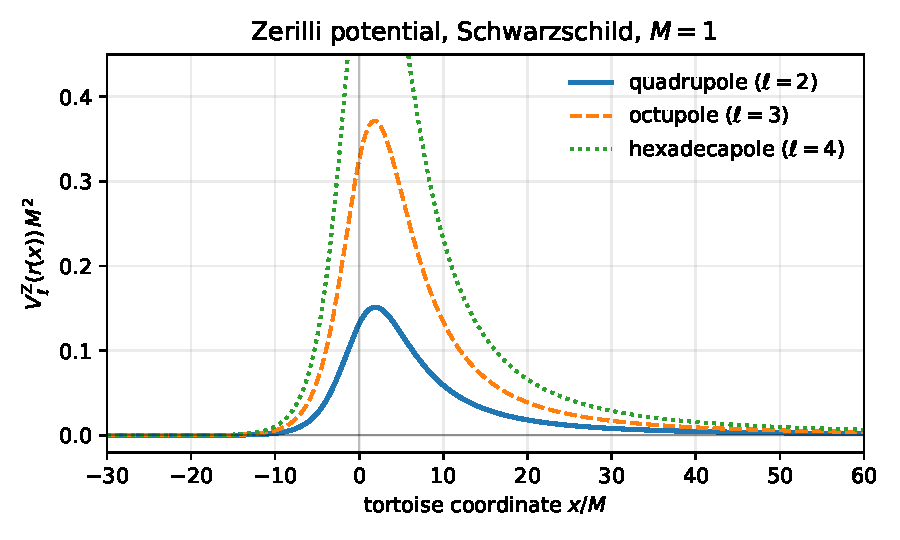
\includegraphics[width=\linewidth]{../outputs/background/zerilli_potential.pdf}
  \caption{Zerilli potential $V_{\ell}^{\mathrm{Z}}(r(x))$ for
  $\ell = 2, 3, 4$ on Schwarzschild ($M = 1$), as a function of the
  tortoise coordinate $x$. The barrier peaks near
  $x \simeq 1.5\,M$ ($r \simeq 3M$, the photon sphere) and decays
  to zero at both the horizon ($x \to -\infty$) and spatial
  infinity ($x \to +\infty$); higher $\ell$ raises the barrier.}
  \label{fig:bg-potential}
\end{minipage}\hfill
\begin{minipage}[t]{0.49\textwidth}
  \centering
  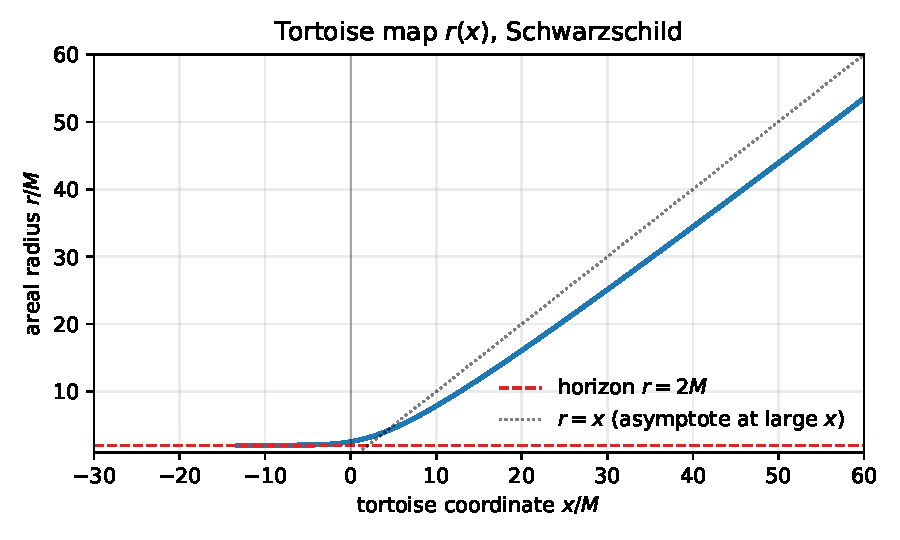
\includegraphics[width=\linewidth]{../outputs/background/tortoise_map.pdf}
  \caption{Tortoise map $r(x)$ for Schwarzschild,
  Eq.~\eqref{eq:tortoise}. The horizon at $r = 2M$ is pushed to
  $x \to -\infty$, and $r(x) \to x$ at large $x$. The PINN
  observer position $\xq = 10\,M$ lies in the asymptotic
  region.}
  \label{fig:bg-tortoise}
\end{minipage}
\end{figure}

A quasinormal mode is a separated solution
$\Phi(t,x) = \mathrm{e}^{-\mathrm{i}\omega t}\,\psi(x)$ of
Eq.~\eqref{eq:zerilli}. Substitution gives the time-independent
Schr\"odinger-like equation
\begin{equation}
  \frac{\mathrm{d}^{2}\psi}{\mathrm{d}x^{2}}
  + \bigl(\omega^{2} - V_{\ell}(r(x))\bigr)\psi(x) \;=\; 0.
  \label{eq:zerilli-freq}
\end{equation}
In the asymptotic regions Eq.~\eqref{eq:zerilli-freq} has
plane-wave solutions $\mathrm{e}^{\pm\mathrm{i}\omega x}$, and
the QNM boundary conditions select modes purely ingoing at the
horizon and purely outgoing at infinity,
\begin{equation}
  \psi(x) \;\to\; \mathrm{e}^{-\mathrm{i}\omega x}\;\;(x \to -\infty),
  \qquad
  \psi(x) \;\to\; \mathrm{e}^{+\mathrm{i}\omega x}\;\;(x \to +\infty).
  \label{eq:qnm-bc}
\end{equation}
Radiation leaves but never enters, so the operator is
non-Hermitian and the admissible frequencies form a discrete
complex spectrum \citep{Berti2009review,KonoplyaZhidenko2011},
\begin{equation}
  \omega_{n} \;=\; \omega_{n}^{R} - \mathrm{i}/\tau_{n},
  \qquad \omega_{n}^{R}, \tau_{n} > 0,
  \label{eq:qnm-omega}
\end{equation}
ordered by overtone index $n=0,1,2,\ldots$ in increasing
damping rate $1/\tau_n$. The real part $\omega_n^{R}$ is the
oscillation frequency and $\tau_n$ the damping time.

For Schwarzschild $\ell = 2$ the fundamental ($n = 0$) and
first overtone ($n = 1$) are
\begin{equation}
  M\omega_{0}^{R} = 0.3737, \quad \tau_{0}/M = 11.241,
  \qquad
  M\omega_{1}^{R} = 0.3467, \quad \tau_{1}/M = 3.651,
  \label{eq:qnm-ref}
\end{equation}
computed to high numerical precision by Leaver's
continued-fraction method \citep{Leaver1985} and tabulated by
\citet{Berti2009review}; every extraction reported in this
paper is benchmarked against them. The fundamental $\ell = 2$
mode dominates the observed ringdown of binary mergers and is
the primary spectroscopy target; the first overtone enters at
sufficient signal-to-noise ratio
\citep{Buonanno2007ringdown,LIGO2016ringdown,Isi2021priors}.
WKB expansions
\citep{SchutzWill1985,IyerWill1987,Konoplya2003wkb} and the
asymptotic-iteration method \citep{Cho2010aim} provide
semi-analytic estimates, while Leaver's continued-fraction
method and Nollert's refinement provide high-accuracy numerical
benchmarks \citep{Leaver1985,Nollert1993}.

\subsection{Kerr perturbations and the Teukolsky equation}
\label{sec:teukolsky-problem}

Schwarzschild is the non-rotating limit. Astrophysical remnants
rotate, and a rotating black hole of mass $M$ and spin
$a = J/M$ is described, in Boyer--Lindquist coordinates, by the
Kerr line element
\begin{equation}
  \begin{aligned}
  \mathrm{d}s^{2} ={}&
    -\left(1 - \frac{2Mr}{\Sigma}\right)\mathrm{d}t^{2}
    - \frac{4 M a r \sin^{2}\!\theta}{\Sigma}\,
       \mathrm{d}t\,\mathrm{d}\varphi \\
    &+ \frac{\Sigma}{\Delta}\,\mathrm{d}r^{2}
    + \Sigma\,\mathrm{d}\theta^{2} \\
    &+ \left(r^{2} + a^{2}
       + \frac{2 M a^{2} r \sin^{2}\!\theta}{\Sigma}\right)
       \sin^{2}\!\theta\,\mathrm{d}\varphi^{2},
  \end{aligned}
  \label{eq:kerr-metric}
\end{equation}
with $\Sigma = r^{2} + a^{2}\cos^{2}\theta$ and
$\Delta = r^{2} - 2Mr + a^{2}$. This reduces to the
Schwarzschild metric Eq.~\eqref{eq:schwarzschild} as
$a \to 0$. The roots of $\Delta$ are the outer and inner
horizons
\begin{equation}
  r_{\pm} = M \pm \sqrt{M^{2} - a^{2}},
  \label{eq:kerr-horizons}
\end{equation}
which merge at extremality $a \to M$. The off-diagonal
$\mathrm{d}t\,\mathrm{d}\varphi$ term is the frame dragging that
distinguishes Kerr from Schwarzschild. We study spins
$a/M \in [0, 0.95]$, stopping short of extremality.

Gravitational perturbations of Kerr do not split into parity
sectors. Instead, gravitational perturbations are described by the
spin-weight $s=-2$ Teukolsky master equation \citep{Teukolsky1973}.
For the gravitational ($s = -2$) field the separable ansatz
$\psi = e^{-i\omega t + i m\varphi}\,
{}_{-2}S_{\ell m}(\theta)\,R(r)$ yields a spheroidal angular
equation, whose eigenfunctions are the spin-weighted spheroidal
harmonics ${}_{-2}S_{\ell m}(\theta; a\omega)$ with separation
constant $\lambda$, and the radial equation
\begin{equation}
  \Delta^{2}\frac{\mathrm{d}}{\mathrm{d}r}\!
    \left(\Delta^{-1}\frac{\mathrm{d}R}{\mathrm{d}r}\right)
  + \left[\frac{K^{2} + 4 i (r - M) K}{\Delta}
          - 8 i \omega r - \lambda\right] R = 0,
  \qquad
  K = (r^{2} + a^{2})\,\omega - a m .
  \label{eq:teukolsky}
\end{equation}
Rotation enters through both $a\omega$ in the angular eigenvalue
and the $a m$ term in $K$, coupling the spectrum to the azimuthal
number $m$. For gravitational perturbations with $s=-2$, the
radial Teukolsky equation is complex-valued. As $a \to 0$,
Eq.~\eqref{eq:teukolsky} reduces to the Bardeen--Press form of
the Schwarzschild perturbation equation, whose gravitational QNM
spectrum agrees with the Regge--Wheeler and Zerilli spectra. The
quasinormal spectrum therefore depends on spin
(Fig.~\ref{fig:kerr-spectrum}). For the prograde modes shown
here, the real frequency $M\omega_{R}$ rises and the damping time
$\tau$ lengthens as $a/M$ increases, so an hFNO trained across
spins must learn this spin dependence.

\begin{figure}[!htbp]
\centering
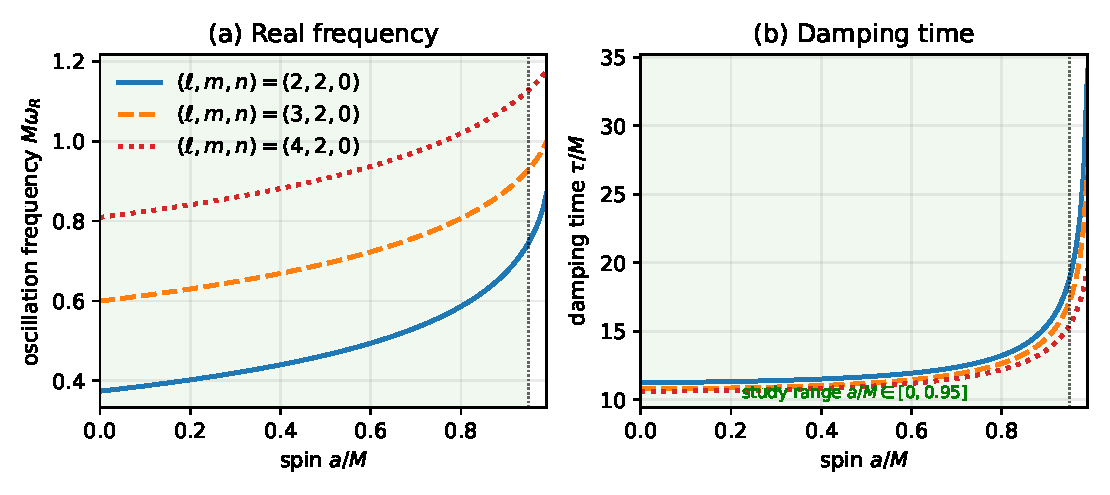
\includegraphics[width=0.92\textwidth]{../outputs/background/kerr_spectrum.pdf}
\caption{Gravitational ($s = -2$) quasinormal spectrum of Kerr
versus spin $a/M$, for the fundamental ($n = 0$) modes
$(\ell, m) = (2,2), (3,2), (4,2)$, computed by Leaver's
continued-fraction method \citep{Leaver1985} through the
\texttt{qnm} package \citep{Stein2019qnm}. (a) The oscillation
frequency $M\omega_{R}$ and (b) the damping time $\tau/M$ both
grow towards extremality, and higher $\ell$ oscillates faster.
The shaded band marks the study range $a/M \in [0, 0.95]$. At
$a = 0$ the $(2,2,0)$ values reproduce the Schwarzschild
reference of Eq.~\eqref{eq:qnm-ref}. We target the $(4,2,0)$
mode, the fastest-oscillating of the three.}
\label{fig:kerr-spectrum}
\end{figure}

\subsection{PINNs and neural-network QNM studies}
\label{sec:bg-pinn}

A physics-informed neural network (PINN) \citep{Raissi2017}
approximates the solution of a differential equation with a
differentiable neural ansatz and trains it by penalising the PDE
residual together with the initial and boundary residuals at
collocation points
\citep{Karniadakis2021piml,Cuomo2022pinnreview}. Automatic
differentiation supplies the derivatives entering the residual
\citep{Baydin2018ad}, so the method avoids finite-difference
stencils but still depends on the sampling strategy, network
architecture, optimiser and relative weighting of the loss terms.
These sensitivities are well known in the PINN literature, where
loss balancing, gradient pathologies and adaptive sampling remain
active topics
\citep{Wang2021gradientpath,Wang2022ntk,McClenny2023sapinn,Wang2022causal,Wu2023adaptive}.
The concrete architecture, loss and training schedule used here
are specified in Sec.~\ref{sec:fwd-pinn}.

\label{sec:bg-prior}
For the present comparison, prior neural-network QNM studies are
best separated by whether they solve an eigenvalue problem
directly or first generate a time-domain waveform.
\citet{Ovgun2021qnmnn} use a feedforward neural-network method
for dS and AdS black-hole QNMs. \citet{Cornell2022pinnqnm}
train a PINN eigenvalue solver for non-rotating black holes and
recover low-lying modes with small errors. \citet{Haddou2023drgt}
apply PINNs to near-extremal black holes in dRGT massive gravity.
\citet{Luna2022teukolskypinn} solve the separated radial and
angular Teukolsky eigenvalue problem for Kerr, hard-enforcing
regularity and QNM boundary behaviour. \citet{Luna2024qnm}
extend the same frequency-domain strategy to modified gravity
with numerical background solutions, while
\citet{Cornell2024rwteukolsky} use supervised PINNs with
labelled eigenfunction data to access higher Regge--Wheeler and
Teukolsky overtones. These studies compute the QNM frequency as
part of the neural solution. They therefore differ from the
present time-domain benchmark, where the learned object is first
the waveform and the QNM estimate is extracted afterwards.

The closest comparator for this dissertation is
\citet{Patel2024pinn}, who solve the time-domain Zerilli and
Regge--Wheeler initial-boundary-value problems with a
fully-connected PINN and then extract QNMs from the observer
waveform. Their reported field error is the main baseline for
the reproduction study, and their extraction procedure provides
the reproduced baseline for our downstream QNM comparison.

\subsection{Neural operators and prior operator-learning work}
\label{sec:bg-fno}

A neural operator learns a map between function spaces rather
than a solution for one fixed PDE instance
\citep{Lu2021deeponet,Li2021fno,Kovachki2023neuralop}. For a
parametric family, it approximates the solution operator
$\mathcal{G}_{\theta}\colon \mathcal{A} \to \mathcal{U}$ and
can then evaluate new parameter draws with one forward pass.
DeepONet represents this map with branch and trunk networks
\citep{Lu2021deeponet}. The Fourier neural operator (FNO)
instead parameterises the integral kernel in Fourier space,
giving spectral convolution layers that can be evaluated across
compatible grid resolutions
\citep{Li2021fno,Kovachki2023neuralop}. Neural operators have
been demonstrated on standard PDE benchmarks including Burgers'
equation, Darcy flow and Navier-Stokes flow
\citep{Li2021fno,Lu2021deeponet,Kovachki2023neuralop}. To our
knowledge, there has been no previous neural-operator
application to the time-domain Regge--Wheeler or Zerilli
problem.

A related line of work combines neural networks with classical
solvers rather than replacing the solver entirely.
Solver-in-the-loop training uses differentiable PDE solvers to
train stable learned corrections \citep{Um2020solverloop}, and
learned corrections to under-resolved fluid solvers can recover
accuracy comparable to much finer simulations at lower cost
\citep{Kochkov2021mlcfd}. The hFNO of
Sec.~\ref{sec:hyb-method} follows this coarse-solver-plus-learned-
correction idea. It uses a coarse finite-difference solve to
carry the wave propagation and an FNO to learn the remaining
coarse-to-fine residual. The residual target is built without fine-grid training
fields by Richardson extrapolation of two coarse solves
\citep{Richardson1911}, and a deterministic gradient gate
focuses the learned correction on the under-resolved wavefronts.

% =====================================================================
% =============================================================
% Section 3: Methods
% =============================================================
\section{Methods}\label{sec:methods}

We consider a forward Schwarzschild PINN, a Schwarzschild hFNO and a
Kerr hFNO. The forward PINN approximates one solution of the Zerilli
initial-boundary-value problem by minimising the equation, initial-data
and boundary-condition residuals. The two hFNOs are trained separately
on Schwarzschild mass and initial-data configurations and on Kerr spin
and initial-pulse configurations. For each configuration, the
finite-difference solver first computes a coarse-grid solution, after
which an FNO returns an additive correction on the output grid. QNM
parameters are extracted from the Schwarzschild waveform at the fixed
code coordinate $\xq=10$ and from the Kerr waveform at $\scri$.
For the canonical $M=1$ configuration, $\xq=10\,M$. The Schwarzschild
analysis uses M1--M5, while the Kerr analysis also uses estimators
defined directly for a complex waveform.

\begin{table}[!htbp]
\centering
\caption{Training configurations for the forward PINN and
Schwarzschild hFNO. All learning rates are $10^{-3}$; hFNO weight
decay is $10^{-6}$.}
\label{tab:train-config}
\footnotesize
\setlength{\tabcolsep}{5pt}
\begin{tabular}{@{}lcc@{}}
\toprule
 & Forward PINN & Schwarzschild hFNO \\
\midrule
Parameters & $4{,}521$ & $1.13\times 10^{6}$ \\
Optimiser  & Adam${\to}$L-BFGS & AdamW \\
Budget     & $10^{4} + 3{\times}10^{4}$ it. & $100$ ep. \\
Batch size & full & $8$ \\
Precision  & \texttt{float64} & \texttt{float32} \\
\bottomrule
\end{tabular}
\end{table}

% --------------------------------------------------------------
\subsection{Schwarzschild Zerilli problem}
\label{sec:fwd-problem}

The canonical Schwarzschild forward problem is the Zerilli equation
Eq.~\eqref{eq:zerilli} with the polar potential
$V_{\ell}^{\mathrm{Z}}$ of Eq.~\eqref{eq:V-zerilli}, evaluated at
$\ell=2$ and $M=1$ on the numerical domain
$x\in[-50,150]\,M$ and $t\in[0,50]\,M$. We use
outgoing Gaussian initial data
\begin{equation}
  \Phi(x,0) = A_0\,\exp\!\left[-\frac{(x-x_0)^2}{\sigma_0^2}\right],
  \qquad
  \partial_t \Phi(x,0) = -\partial_x \Phi(x,0)
  = \frac{2(x-x_0)}{\sigma_0^2}\,\Phi(x,0),
  \label{eq:ic}
\end{equation}
with $A_0 = 1$, $x_0 = 4\,M$ and $\sigma_0 = 5\,M$. This choice
enforces the outgoing flat-space condition
$(\partial_t+\partial_x)\Phi=0$ at $t=0$, so the initial packet
propagates towards spatial infinity before scattering from the
Zerilli potential. It differs only in the initial velocity profile
from the setup of \citet{Patel2024pinn}, while retaining their
amplitude, centre and width. At the finite radial boundaries
$x=x_{\min}$ and $x=x_{\max}$, we impose the first-order Sommerfeld
conditions
\begin{equation}
  (\partial_t - \partial_x)\Phi\bigl|_{x=x_{\min}} = 0, \qquad
  (\partial_t + \partial_x)\Phi\bigl|_{x=x_{\max}} = 0,
  \label{eq:bc-sommerfeld}
\end{equation}
These are the finite-domain outgoing conditions used by
\citet{Patel2024pinn}. They approximate ingoing radiation at the
horizon side and outgoing radiation at the outer boundary, rather
than the frequency-domain QNM eigenvalue conditions imposed at
$x\to\pm\infty$. The characteristic travel times from the packet
centre to the two boundaries are
\begin{equation}
  t_{R} = x_{\max} - x_0 = 146\,M, \qquad
  t_{L} = x_0 - x_{\min} = 54\,M,
  \label{eq:bc-arrival}
\end{equation}
Both times exceed the PINN evaluation window. The PINN boundary losses
therefore enforce the Sommerfeld conditions outside the domain of
dependence of the observer waveform over $0\leq t\leq50\,M$, while the
FD reference is insensitive to the boundaries over this interval.

The Zerilli reference field (Fig.~\ref{fig:waveform-3d}) is computed
with a method-of-lines finite-difference (FD) scheme using second-order centred
spatial differences, second-order one-sided boundary closures and
fourth-order Runge--Kutta time stepping, using $\Delta x = 0.2\,M$
and $\Delta t = 0.1\,M$. It is used as the numerical reference for
the Zerilli PINN field errors and as the finite-difference waveform
used to evaluate the QNM estimators. The Leaver values
$M\omega_0^R = 0.3737$,
$\tau_0/M = 11.241$ (fundamental) and $M\omega_1^R = 0.3467$,
$\tau_1/M = 3.651$ (first overtone) of Eq.~\eqref{eq:qnm-ref}
are used for percentage-error reporting.
The Regge--Wheeler reproduction uses the same domain, initial data,
boundary conditions, FD scheme and extraction protocol with
$V_{\ell}^{\mathrm{Z}}$ replaced by the axial Regge--Wheeler
potential. The later Schwarzschild extensions use the Zerilli
equation. The Regge--Wheeler and Zerilli equations have the same QNM
spectrum.

\begin{figure}[!htbp]
\centering
\begin{minipage}[t]{0.49\textwidth}
  \centering
  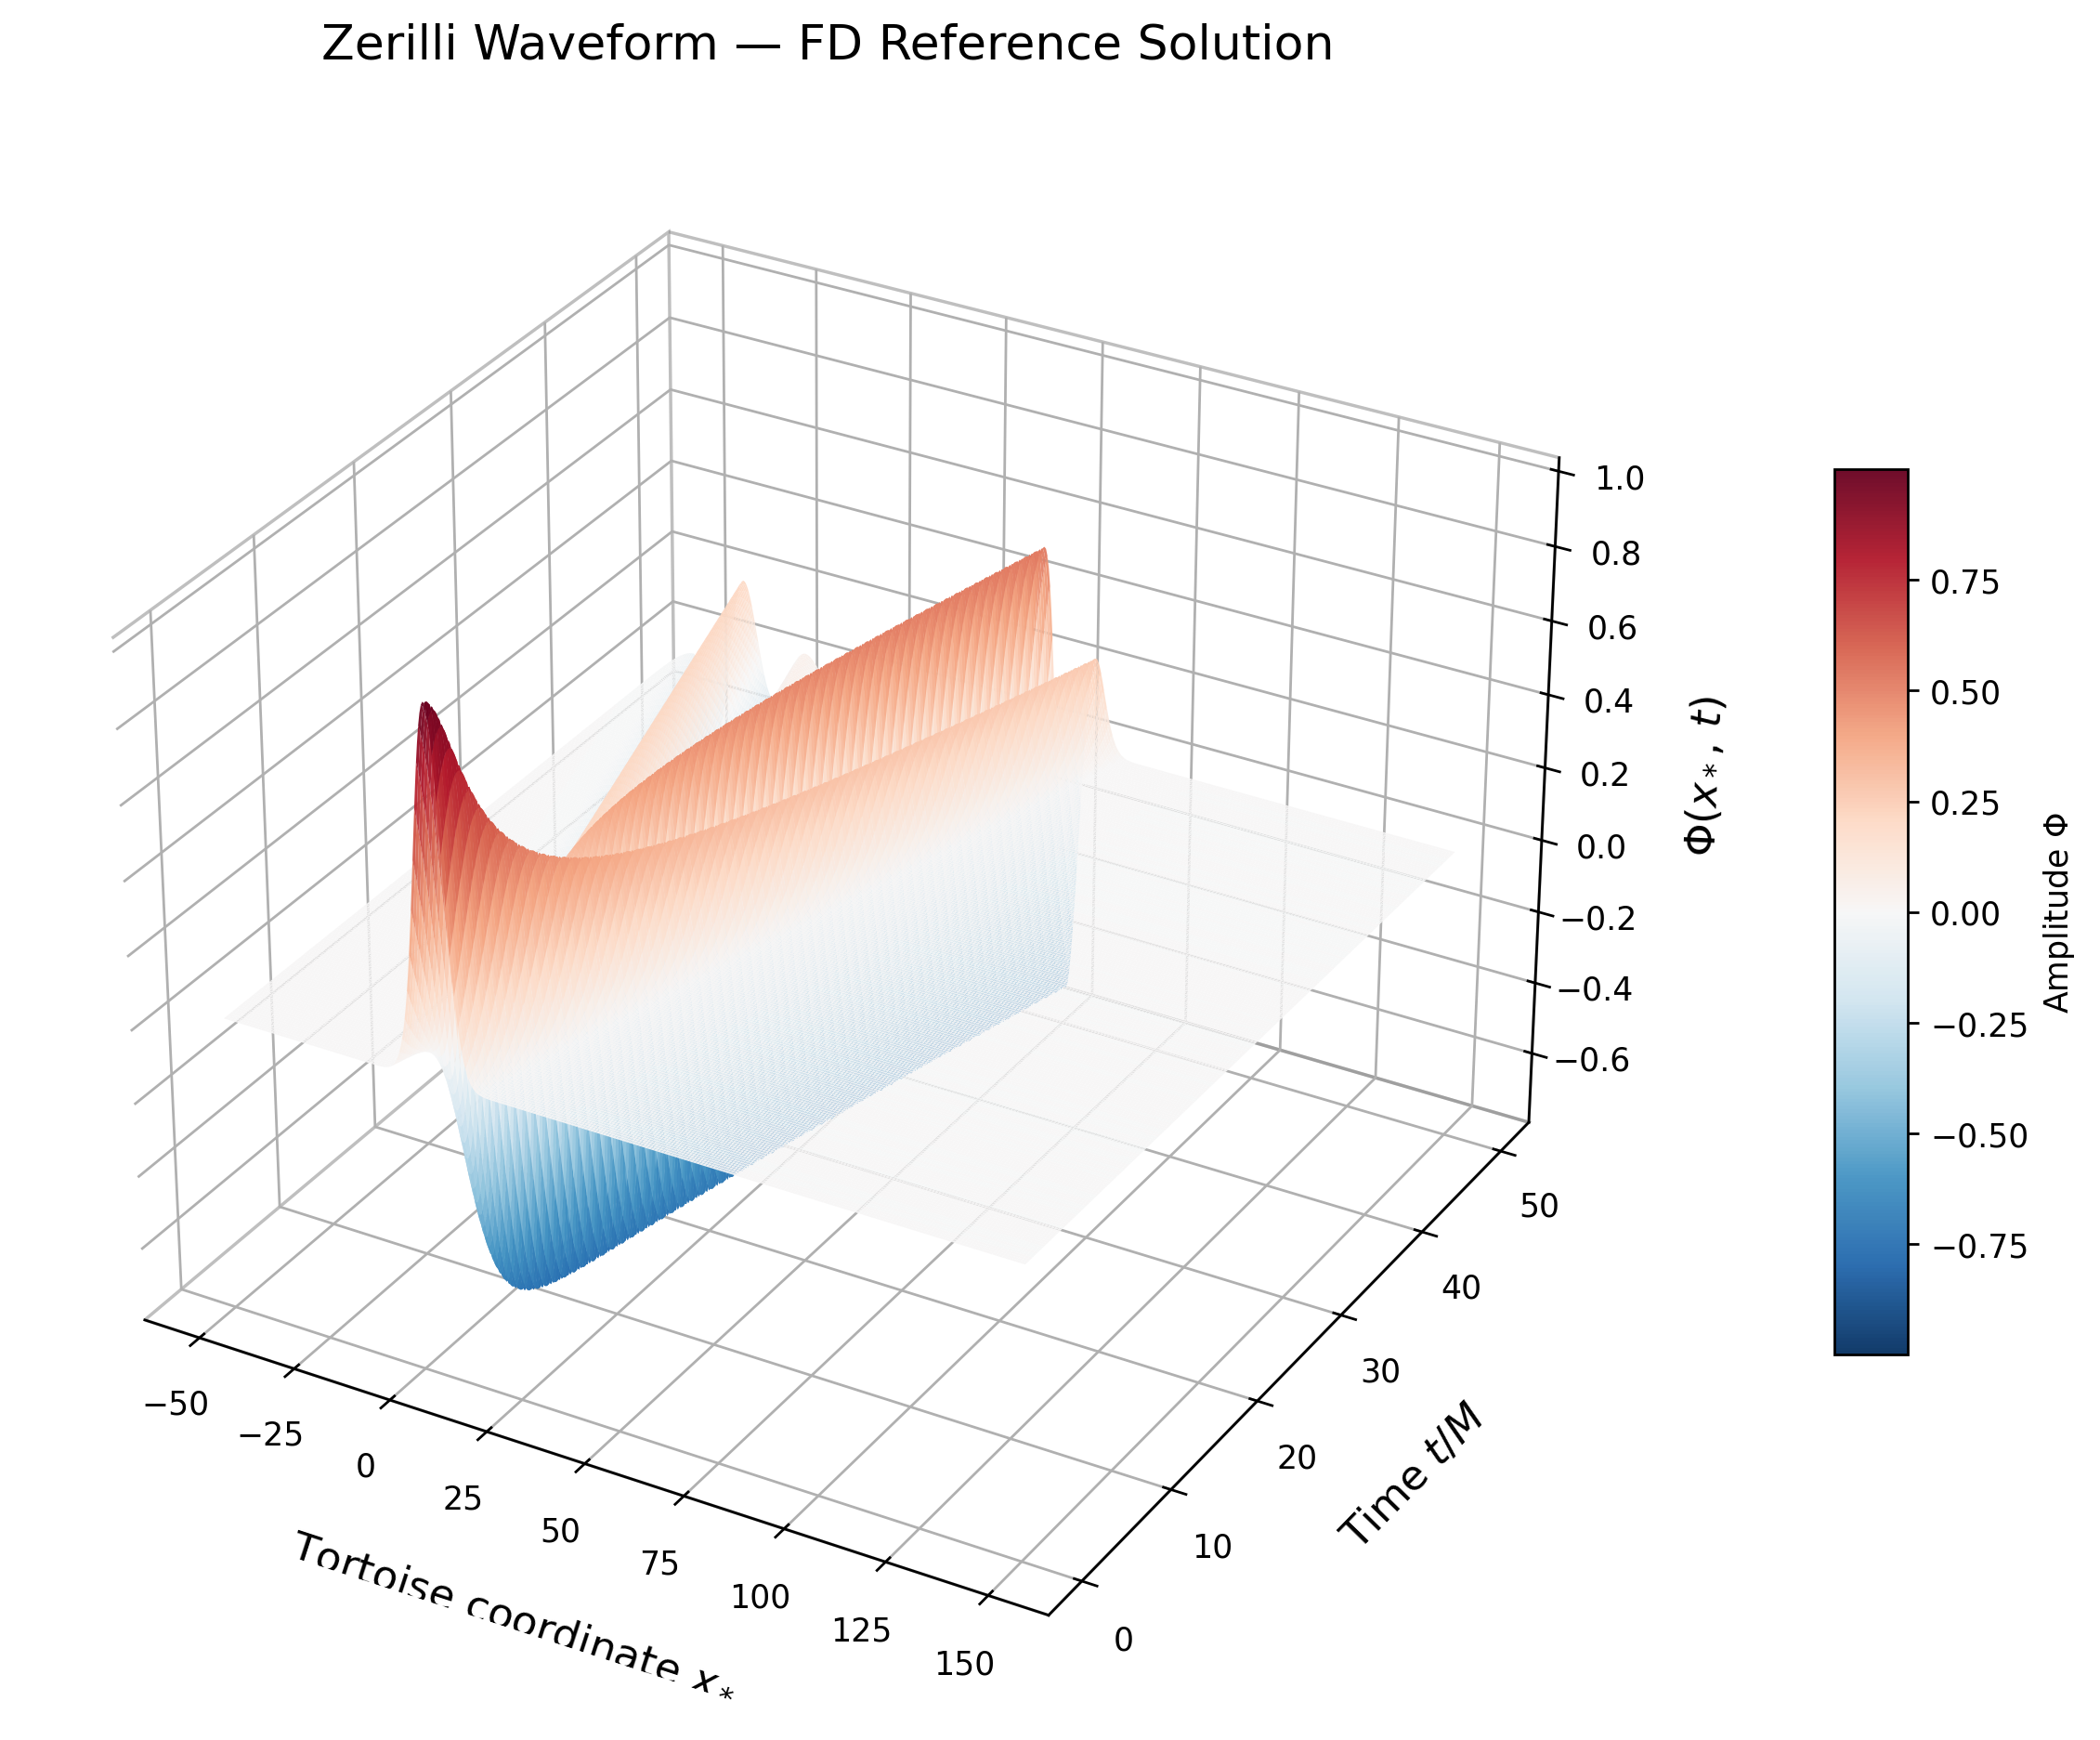
\includegraphics[width=\linewidth]{../outputs/pinn/waveform_3d_full.png}
  \subcaption{Full domain $x \in [-50, 150]\,M$, $t \in [0, 50]\,M$.
  The right-moving free pulse from the outgoing initial condition
  is visible as the diagonal ridge propagating to the right (towards
  infinity); the left-moving ridge towards the horizon is the
  back-scattered component generated by the photon-sphere barrier.}
  \label{fig:waveform-3d-full}
\end{minipage}\hfill
\begin{minipage}[t]{0.49\textwidth}
  \centering
  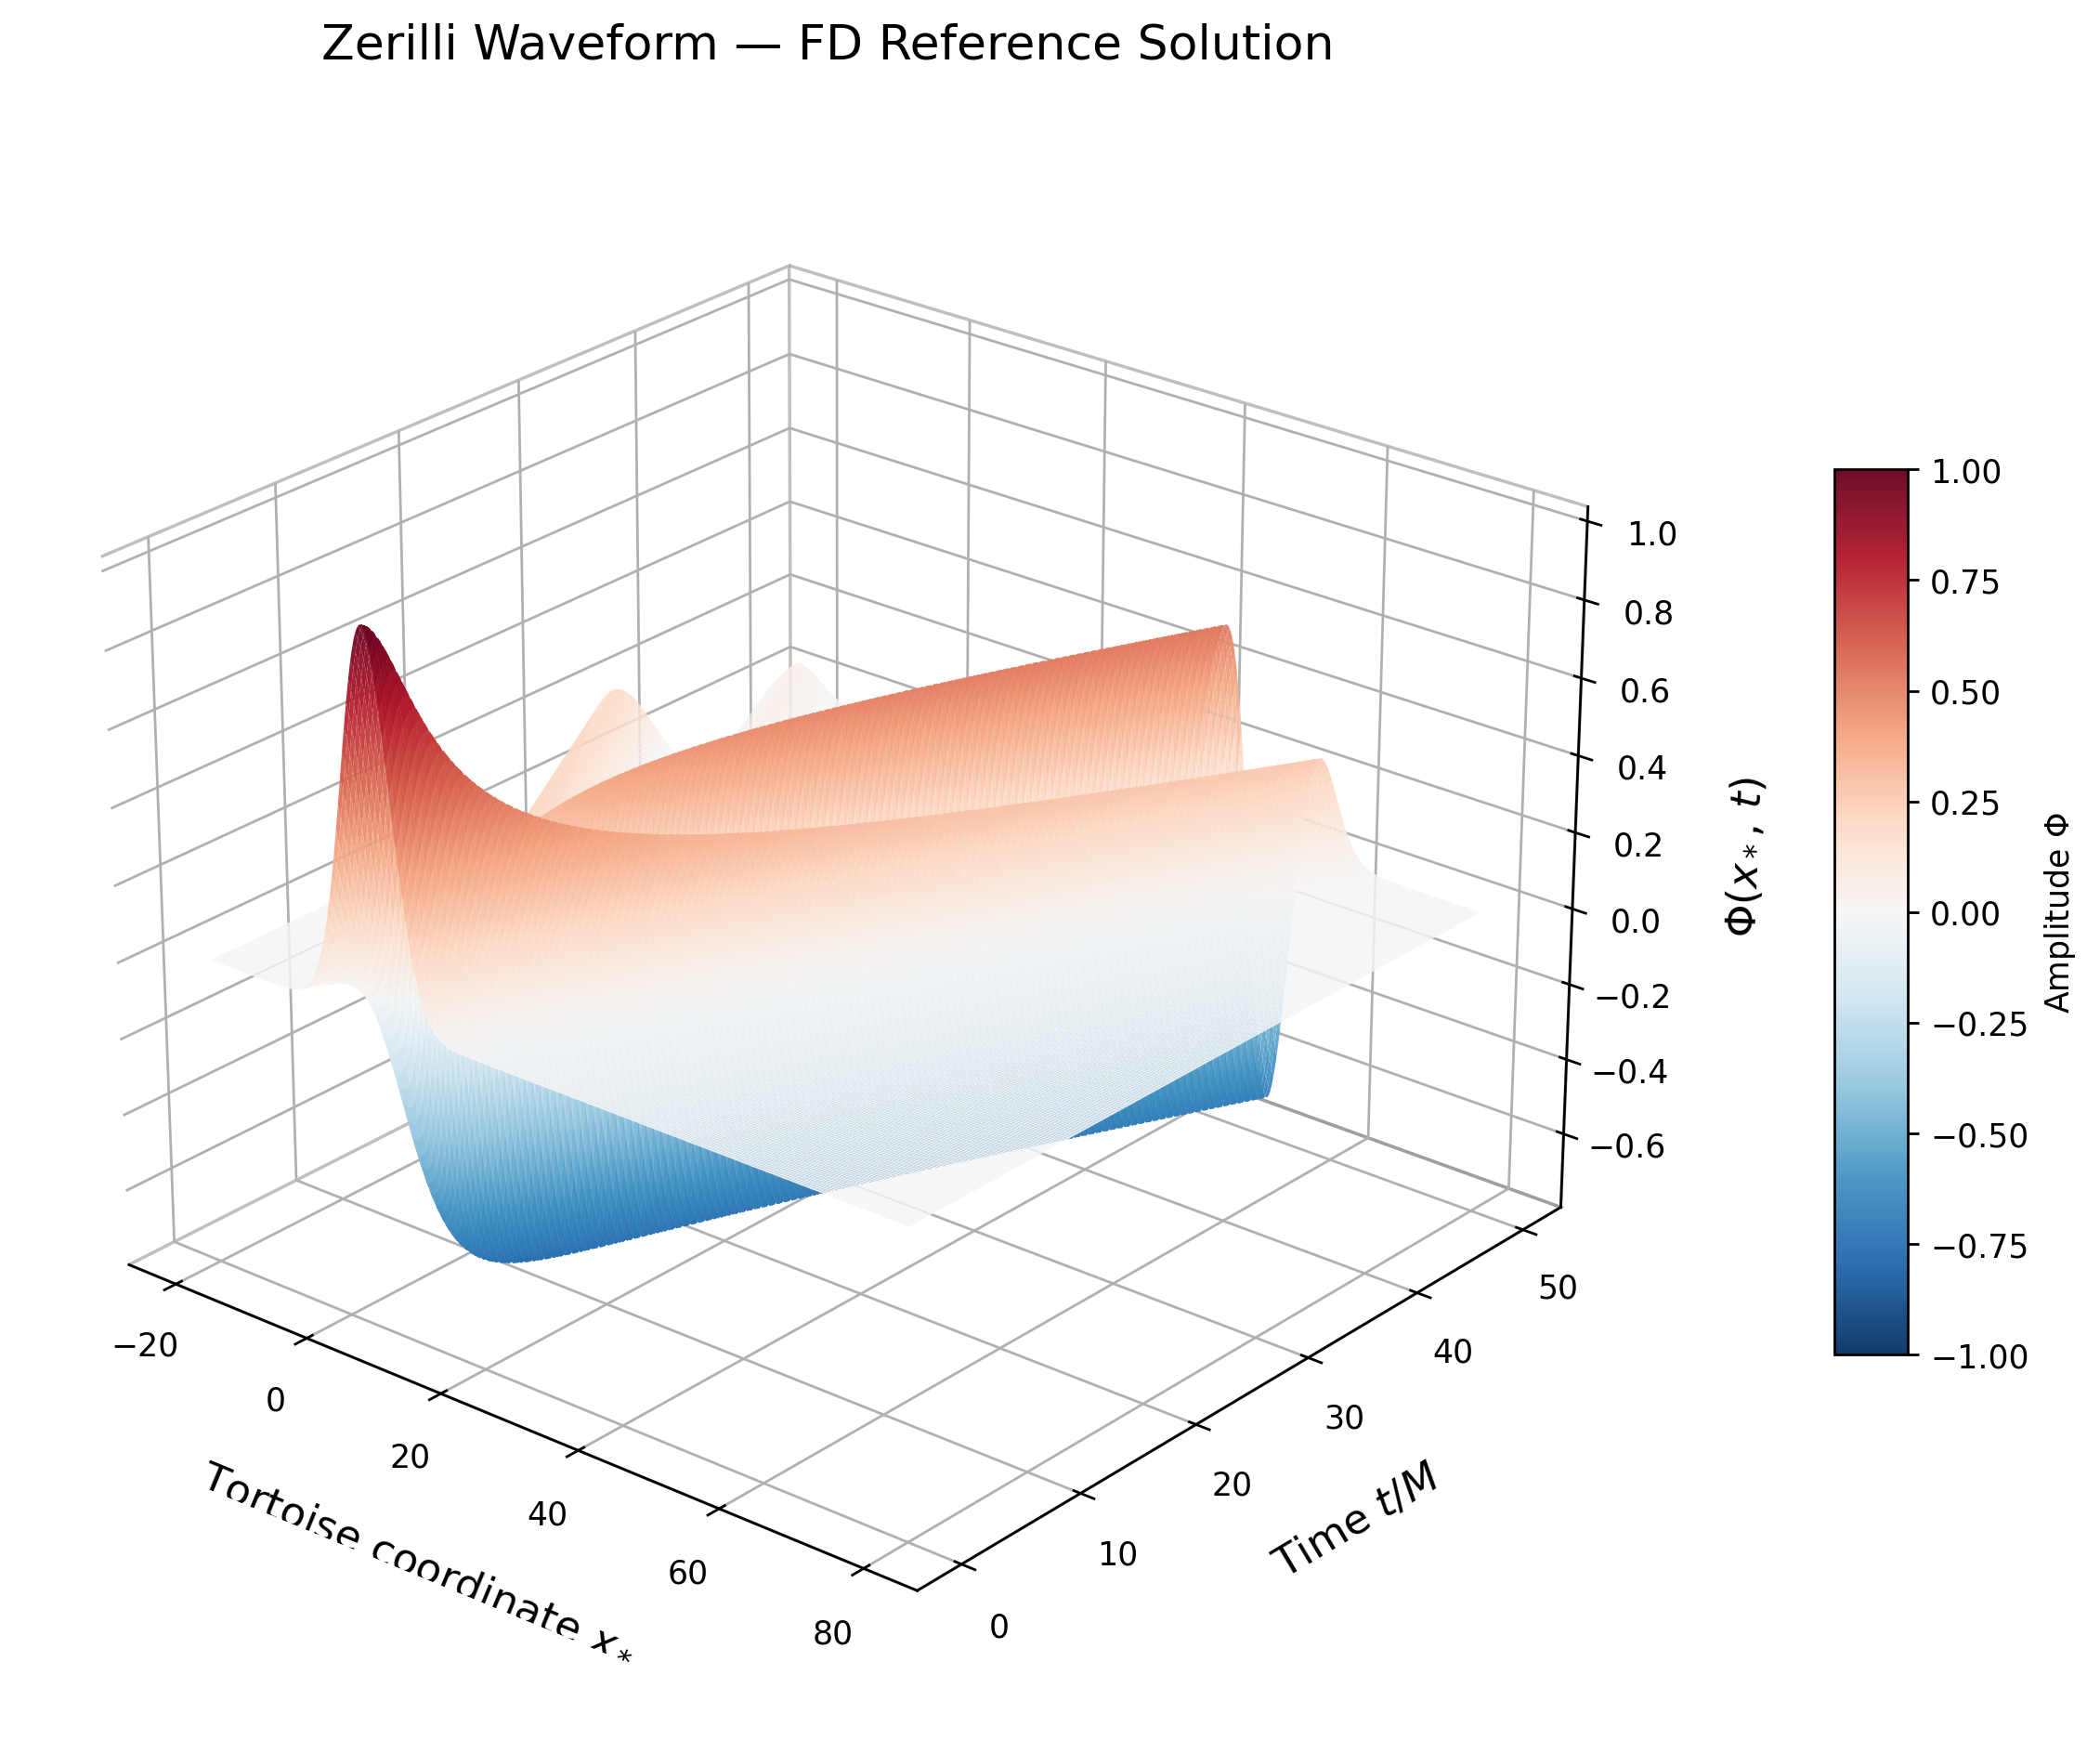
\includegraphics[width=\linewidth]{../outputs/pinn/waveform_3d_zoom.png}
  \subcaption{Zoom around the observer region $x \in [-20,80]\,M$. The
  ringdown is visible as the small-amplitude decaying oscillation
  near $x \simeq 10\,M$ for $t \gtrsim 10\,M$, lying between
  the right-moving free pulse and the back-scattered left-mover.}
  \label{fig:waveform-3d-zoom}
\end{minipage}
\caption{FD reference field $\Phi_{\mathrm{FD}}(x,t)$ for the
Schwarzschild $\ell=2$ Zerilli problem, generated by the fourth-order
Runge--Kutta method-of-lines integration of
Eq.~\eqref{eq:zerilli} with the initial data of
Eq.~\eqref{eq:ic} and the Sommerfeld boundaries of
Eq.~\eqref{eq:bc-sommerfeld}. The Zerilli PINN field-accuracy
metrics in Sec.~\ref{sec:results} are computed against this
reference.}
\label{fig:waveform-3d}
\end{figure}

% --------------------------------------------------------------
\subsection{Forward PINN}
\label{sec:fwd-pinn}

We implement the forward PINN \citep{Raissi2017} in DeepXDE
\citep{Lu2021deepxde} with the PyTorch backend
\citep{Paszke2019pytorch}. Following \citet{Patel2024pinn}, it uses a
fully connected $[80,40,20,10]$ $\tanh$ network with Glorot-uniform
initialisation, coordinates scaled linearly to $[-1,1]^2$, and the
bounded output $\Phi_\theta=A_0\tanh\hat y$. The architecture is held
fixed between the reproduction and enhanced runs, so their comparison
isolates the training schedule, collocation sampling and extraction
protocol. The network has $4{,}521$ trainable parameters.

At each coordinate pair $(x,t)$, the network returns the field value
$\Phi_\theta(x,t)$. Automatic differentiation supplies the derivatives
used to evaluate the Zerilli, initial-data and boundary residuals.
Consequently, no FD field values enter the PINN loss; the FD solution
is retained only for evaluation.

\begin{figure}[!htbp]
\centering
\resizebox{\textwidth}{!}{%
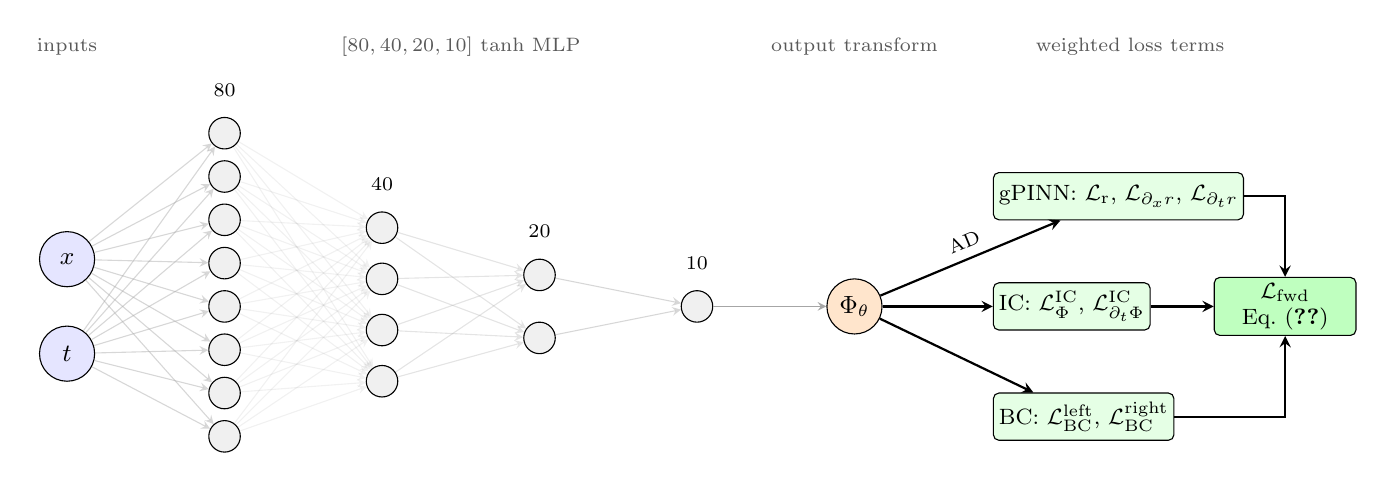
\begin{tikzpicture}[
  node distance=10mm and 12mm,
  every node/.style={font=\small},
  inp/.style={circle, draw, fill=blue!10, minimum size=7mm, inner sep=0pt},
  hid/.style={circle, draw, fill=gray!12, minimum size=4mm, inner sep=0pt},
  outn/.style={circle, draw, fill=orange!20, minimum size=7mm, inner sep=0pt},
  loss/.style={rectangle, draw, fill=green!10, rounded corners=2pt,
               minimum height=6mm, minimum width=18mm, inner sep=2pt,
               align=center, font=\footnotesize},
  arr/.style={->, >=stealth, thin, gray!70},
]
  % Inputs
  \node[inp] (x) at (0, 0) {$x$};
  \node[inp] (t) at (0, -1.2) {$t$};

  % Layer geometry: visually decreasing column heights to reflect 80, 40, 20, 10.
  % Layer 1: 8 nodes, Layer 2: 4 nodes, Layer 3: 2 nodes, Layer 4: 1 node.
  % Use vertical spacing 0.45 cm between nodes; centre each column at y=-0.6.
  \def\xL{2.0}
  \def\xLii{4.0}
  \def\xLiii{6.0}
  \def\xLiv{8.0}

  % Layer 1: 8 nodes, ys from +1.6 to -2.8 (step 0.55)
  \foreach \k/\y in {1/1.6, 2/1.05, 3/0.5, 4/-0.05, 5/-0.6, 6/-1.15, 7/-1.7, 8/-2.25}{
    \node[hid] (a\k) at (\xL, \y) {};
  }
  % Layer 2: 4 nodes, centred at y=-0.6, spacing 0.65
  \foreach \k/\y in {1/0.4, 2/-0.25, 3/-0.9, 4/-1.55}{
    \node[hid] (b\k) at (\xLii, \y) {};
  }
  % Layer 3: 2 nodes
  \foreach \k/\y in {1/-0.2, 2/-1.0}{
    \node[hid] (c\k) at (\xLiii, \y) {};
  }
  % Layer 4: 1 node
  \node[hid] (d1) at (\xLiv, -0.6) {};

  % Layer width labels
  \node[font=\scriptsize] at (\xL, 2.15) {$80$};
  \node[font=\scriptsize] at (\xLii, 0.95) {$40$};
  \node[font=\scriptsize] at (\xLiii, 0.35) {$20$};
  \node[font=\scriptsize] at (\xLiv, -0.05) {$10$};

  % Output
  \node[outn] (phi) at (10.0, -0.6) {$\Phi_\theta$};

  % Connections: fully connected between adjacent shown columns,
  % so every node carries at least one edge (dense-net appearance).
  \foreach \src in {x, t}
    \foreach \dst in {a1,a2,a3,a4,a5,a6,a7,a8}
      \draw[arr, opacity=0.45] (\src) -- (\dst);
  \foreach \a in {1,2,3,4,5,6,7,8}
    \foreach \b in {1,2,3,4}
      \draw[arr, opacity=0.16] (a\a) -- (b\b);
  \foreach \a in {1,2,3,4}
    \foreach \b in {1,2}
      \draw[arr, opacity=0.30] (b\a) -- (c\b);
  \foreach \a in {1,2}
      \draw[arr, opacity=0.45] (c\a) -- (d1);
  \draw[arr] (d1) -- (phi);

  % Loss boxes on the right
  \node[loss, right=14mm of phi, yshift=14mm] (lpde)
    {gPINN: $\mathcal{L}_{\mathrm{r}},\,\mathcal{L}_{\partial_x r},\,\mathcal{L}_{\partial_t r}$};
  \node[loss, right=14mm of phi] (lic)
    {IC: $\mathcal{L}_{\Phi}^{\mathrm{IC}},\,\mathcal{L}_{\partial_t\Phi}^{\mathrm{IC}}$};
  \node[loss, right=14mm of phi, yshift=-14mm] (lbc)
    {BC: $\mathcal{L}_{\mathrm{BC}}^{\mathrm{left}},\,\mathcal{L}_{\mathrm{BC}}^{\mathrm{right}}$};
  \draw[arr, thick, black] (phi) -- (lpde) node[midway, above, font=\scriptsize, sloped] {AD};
  \draw[arr, thick, black] (phi) -- (lic);
  \draw[arr, thick, black] (phi) -- (lbc);

  % Sum to total loss
  \node[loss, fill=green!25, right=8mm of lic] (ltot)
    {$\mathcal{L}_{\mathrm{fwd}}$\\Eq.~\eqref{eq:loss-fwd}};
  \draw[arr, thick, black] (lpde) -| (ltot);
  \draw[arr, thick, black] (lic) -- (ltot);
  \draw[arr, thick, black] (lbc) -| (ltot);

  % Section labels (placed above the layer columns).
  \node[font=\scriptsize, gray!70!black] at (0.0, 2.7) {inputs};
  \node[font=\scriptsize, gray!70!black] at (5.0, 2.7) {$[80,40,20,10]$ tanh MLP};
  \node[font=\scriptsize, gray!70!black] at (10.0, 2.7) {output transform};
  \node[font=\scriptsize, gray!70!black] at (13.5, 2.7) {weighted loss terms};
\end{tikzpicture}}
\caption{Forward PINN architecture used in this work. The physical
inputs $(x,t)$ are linearly normalised and passed through a fully
connected $[80,40,20,10]$ $\tanh$ network with $4{,}521$ trainable
parameters, whose scalar output is wrapped in the tanh envelope
$\Phi_\theta(x,t) = A\tanh(\hat y(x,t))$ with $A = 1$. Spatial and
temporal derivatives required by the Zerilli PDE residual
$\mathcal{L}_{\mathrm{r}}$ of Eq.~\eqref{eq:loss-fwd} and its
gradient augmentations $\mathcal{L}_{\partial_x r},
\mathcal{L}_{\partial_t r}$ (gPINN, \citealt{Yu2022gpinn}) are
computed by automatic differentiation; the IC residuals
$\mathcal{L}_{\Phi}^{\mathrm{IC}}, \mathcal{L}_{\partial_t\Phi}^{\mathrm{IC}}$ and the left/right BC residuals
$\mathcal{L}_{\mathrm{BC}}^{\mathrm{left}}, \mathcal{L}_{\mathrm{BC}}^{\mathrm{right}}$ enter as additional weighted terms with
$\boldsymbol{\lambda} = (100,100,100,1,100,1,1)$
(Eq.~\eqref{eq:weights}).}
\label{fig:fwd-pinn-arch}
\end{figure}

Let $r_\theta(x,t) \equiv \partial_t^2\Phi_\theta -
\partial_x^2\Phi_\theta + V_\ell\,\Phi_\theta$ be the pointwise
residual of Eq.~\eqref{eq:zerilli}, with
$V_\ell=V_\ell^{\mathrm{Z}}$ for the Zerilli runs. The loss is the
weighted mean-squared sum of the PDE, initial-data and boundary
residuals, augmented by the two gradient-enhanced PINN terms
\citep{Yu2022gpinn},
\begin{equation}
  \mathcal{L}_{\mathrm{fwd}}
  = \lambda_{r}     \Lpde
  + \lambda_{r_x}   \mathcal{L}_{\partial_x r}
  + \lambda_{r_t}   \mathcal{L}_{\partial_t r}
  + \lambda_{\mathrm{IC}} \mathcal{L}_{\Phi}^{\mathrm{IC}}
  + \lambda_{\mathrm{IV}} \mathcal{L}_{\partial_t\Phi}^{\mathrm{IC}}
  + \lambda_{\mathrm{BL}} \mathcal{L}_{\mathrm{BC}}^{\mathrm{left}}
  + \lambda_{\mathrm{BR}} \mathcal{L}_{\mathrm{BC}}^{\mathrm{right}}.
  \label{eq:loss-fwd}
\end{equation}
The seven mean-squared component losses are
\begin{align}
  \Lpde &= \frac{1}{N_r}\sum_{(x,t)\in\mathcal{X}_r}
            r_\theta(x,t)^{2},
  & \mathcal{L}_{\partial_x r} &= \frac{1}{N_r}\sum_{(x,t)\in\mathcal{X}_r}
            \bigl(\partial_x r_\theta(x,t)\bigr)^{2},
  \nonumber\\
  \mathcal{L}_{\partial_t r} &= \frac{1}{N_r}\sum_{(x,t)\in\mathcal{X}_r}
            \bigl(\partial_t r_\theta(x,t)\bigr)^{2},
  & \mathcal{L}_{\Phi}^{\mathrm{IC}} &= \frac{1}{N_i}\sum_{x\in\mathcal{X}_i}
            \bigl(\Phi_\theta(x,0)-\Phi(x,0)\bigr)^{2},
  \nonumber\\
  \mathcal{L}_{\partial_t\Phi}^{\mathrm{IC}}
     &= \frac{1}{N_i}\sum_{x\in\mathcal{X}_i}
        \bigl(\partial_t\Phi_\theta(x,0)-\partial_t\Phi(x,0)\bigr)^{2},
  & \mathcal{L}_{\mathrm{BC}}^{\mathrm{left}}
     &= \frac{1}{N_b}\sum_{t\in\mathcal{X}_b^{L}}
        \bigl((\partial_t-\partial_x)\Phi_\theta(x_{\min},t)\bigr)^{2},
  \nonumber\\
  \mathcal{L}_{\mathrm{BC}}^{\mathrm{right}}
     &= \frac{1}{N_b}\sum_{t\in\mathcal{X}_b^{R}}
        \bigl((\partial_t+\partial_x)\Phi_\theta(x_{\max},t)\bigr)^{2},
  & &
  \label{eq:loss-components}
\end{align}
These terms follow \citet[Eqs.~(4)--(10)]{Patel2024pinn}. We use
$N_r=32{,}000$, $N_i=800$ and $N_b=400$ total boundary points.
\citet{Patel2024pinn} describe $400$ points per boundary, which is the
only collocation-count difference in the reproduction. The two
gradient terms penalise spatial and temporal variation of the PDE
residual, following \citet{Yu2022gpinn}. The
forward-PINN weight vector is
\begin{equation}
  \boldsymbol{\lambda}
  = (\lambda_{r},\lambda_{r_x},\lambda_{r_t},\lambda_{\mathrm{IC}},
     \lambda_{\mathrm{IV}},\lambda_{\mathrm{BL}},\lambda_{\mathrm{BR}})
  = (100,\,100,\,100,\,1,\,100,\,1,\,1),
  \label{eq:weights}
\end{equation}
following \citet{Patel2024pinn}. The larger
$\lambda_{\mathrm{IV}}=100$ weights the initial-velocity residual,
which Patel et al. identify as important for controlling phase drift.
The unit Sommerfeld weights are consistent with the causal remoteness
of the finite boundaries in Eq.~\eqref{eq:bc-arrival}.

The reproduction run uses the optimiser schedule of
\citet{Patel2024pinn}, namely Adam \citep{Kingma2015adam} for
$10^4$ iterations followed by L-BFGS \citep{Liu1989lbfgs} for
$1.5\times10^4$ iterations. The enhanced forward PINN keeps Adam
fixed and doubles the L-BFGS budget to $3\times10^4$ iterations
(Table~\ref{tab:train-config}), since the loss continues to decrease
through iteration $\sim 25{,}000$. All PINN training is full-batch
and uses double precision; in single precision the L-BFGS phase
stalled in our runs. During the Adam phase of the enhanced run, every
$1{,}000$ optimiser iterations the greedy resampler
\citep{Lu2021deepxde,Wu2023adaptive} scores $10^5$ uniformly drawn
candidates by the primary PDE residual $|r_\theta|$ and replaces the
interior collocation set with $0.3N_r$ highest-residual points and
$0.7N_r$ uniformly drawn points. The uniform component preserves
coverage away from the wavefront.

% --------------------------------------------------------------
\subsection{The Schwarzschild hFNO}
\label{sec:hyb-method}

Unlike the per-instance PINN, the hFNO is trained on the sampled
$(M,x_0,\sigma)$ configurations to approximate the
discretisation-error correction for each configuration. For a
parameter triple
$q=(M,x_0,\sigma)$, let $\Phi_k^{\mathrm c}(q)$ denote the full FD
field computed with grid factor $k$, and define the upsampled
deployment prior $P(q)=\mathcal U\Phi_4^{\mathrm c}(q)$. The
corresponding map is
\begin{equation}
  \mathcal G_\theta^{\mathrm{hyb}}(q)
  =P(q)+g[P(q)]\,\mathcal H_\theta(X(q)),
  \label{eq:hyb-map}
\end{equation}
where $\mathcal H_\theta$ returns an additive correction on the
same fine $(t,x)$ grid as $P$.

The FNO does not advance the Zerilli equation in time. The FD solver
computes the coarse-grid finite-difference solution on the full
$(t,x)$ domain before the FNO returns its correction in a single
forward pass. This differs from
recurrent solver-in-the-loop training, which modifies each numerical
step \citep{Um2020solverloop,Kochkov2021mlcfd}. The FD fields are
precomputed and no gradients pass through the solver.

During training, for each parameter triple, the corresponding $k=4$
and $k=2$ fields form a Richardson-extrapolated field. The
gated FNO output is fitted to the difference between that estimate
and $P$. The fine FD reference field
does not enter the optimisation objective and is used only to evaluate
the reconstructed field. At inference, the $k=2$ solve, Richardson
construction and fine reference field are absent. A new configuration requires
one $k=4$ solve, quintic upsampling and one FNO evaluation.
The training tensors and canonical evaluation use quintic
interpolation. The archived $100$-configuration population evaluation
uses the legacy cubic interpolation path; its reported field and QNM
statistics therefore refer to that evaluation path.

The coordinate grid, $x_0$, $\sigma$ and $\xq$ are fixed code
coordinates while $M$ varies. Only the canonical $M=1$ configuration
identifies these numerical coordinate values directly with units of
$M$.

\begin{table}[!htbp]
\centering
\caption{Schwarzschild hFNO architecture, parameter domain and
dataset.}
\label{tab:surrogate-config}
\footnotesize
\setlength{\tabcolsep}{5pt}
\begin{tabular}{@{}lc@{}}
\toprule
 & Schwarzschild hFNO \\
\midrule
Domain $x\times t$ (code coordinates) & $[-50,150]\times[0,100]$ \\
Grid $N_{x}\times N_{t}$ (fine) & $1001\times 1001$ \\
Coarse grids & $k{=}4$ prior; $k{=}2,4$ Richardson pair \\
Input channels & $5$ \\
Hidden channels $h$ & $32$ \\
Fourier modes $(K_{t},K_{x})$ & $(16,32)$ \\
Domain padding & $0.10$ \\
Parameters & $1.13\times 10^{6}$ \\
$M$ & $\mathrm{Unif}[0.8,1.2]$ \\
$x_{0}$ & $\mathrm{Unif}[2,6]$ \\
$\sigma$ & $\mathrm{Unif}[3,7]$ \\
Samples (Sobol seed $0$) & $1000/100/100$ \\
Training seed & $1234$ \\
Loss & Eq.~\eqref{eq:hyb-loss} \\
Observer $\xq$ (code coordinate) & $10$ \\
Canonical $(M,x_{0},\sigma)$ & $(1,4,5)$ \\
\bottomrule
\end{tabular}
\end{table}

\begin{figure}[!htbp]
\centering
\resizebox{0.78\textwidth}{!}{%
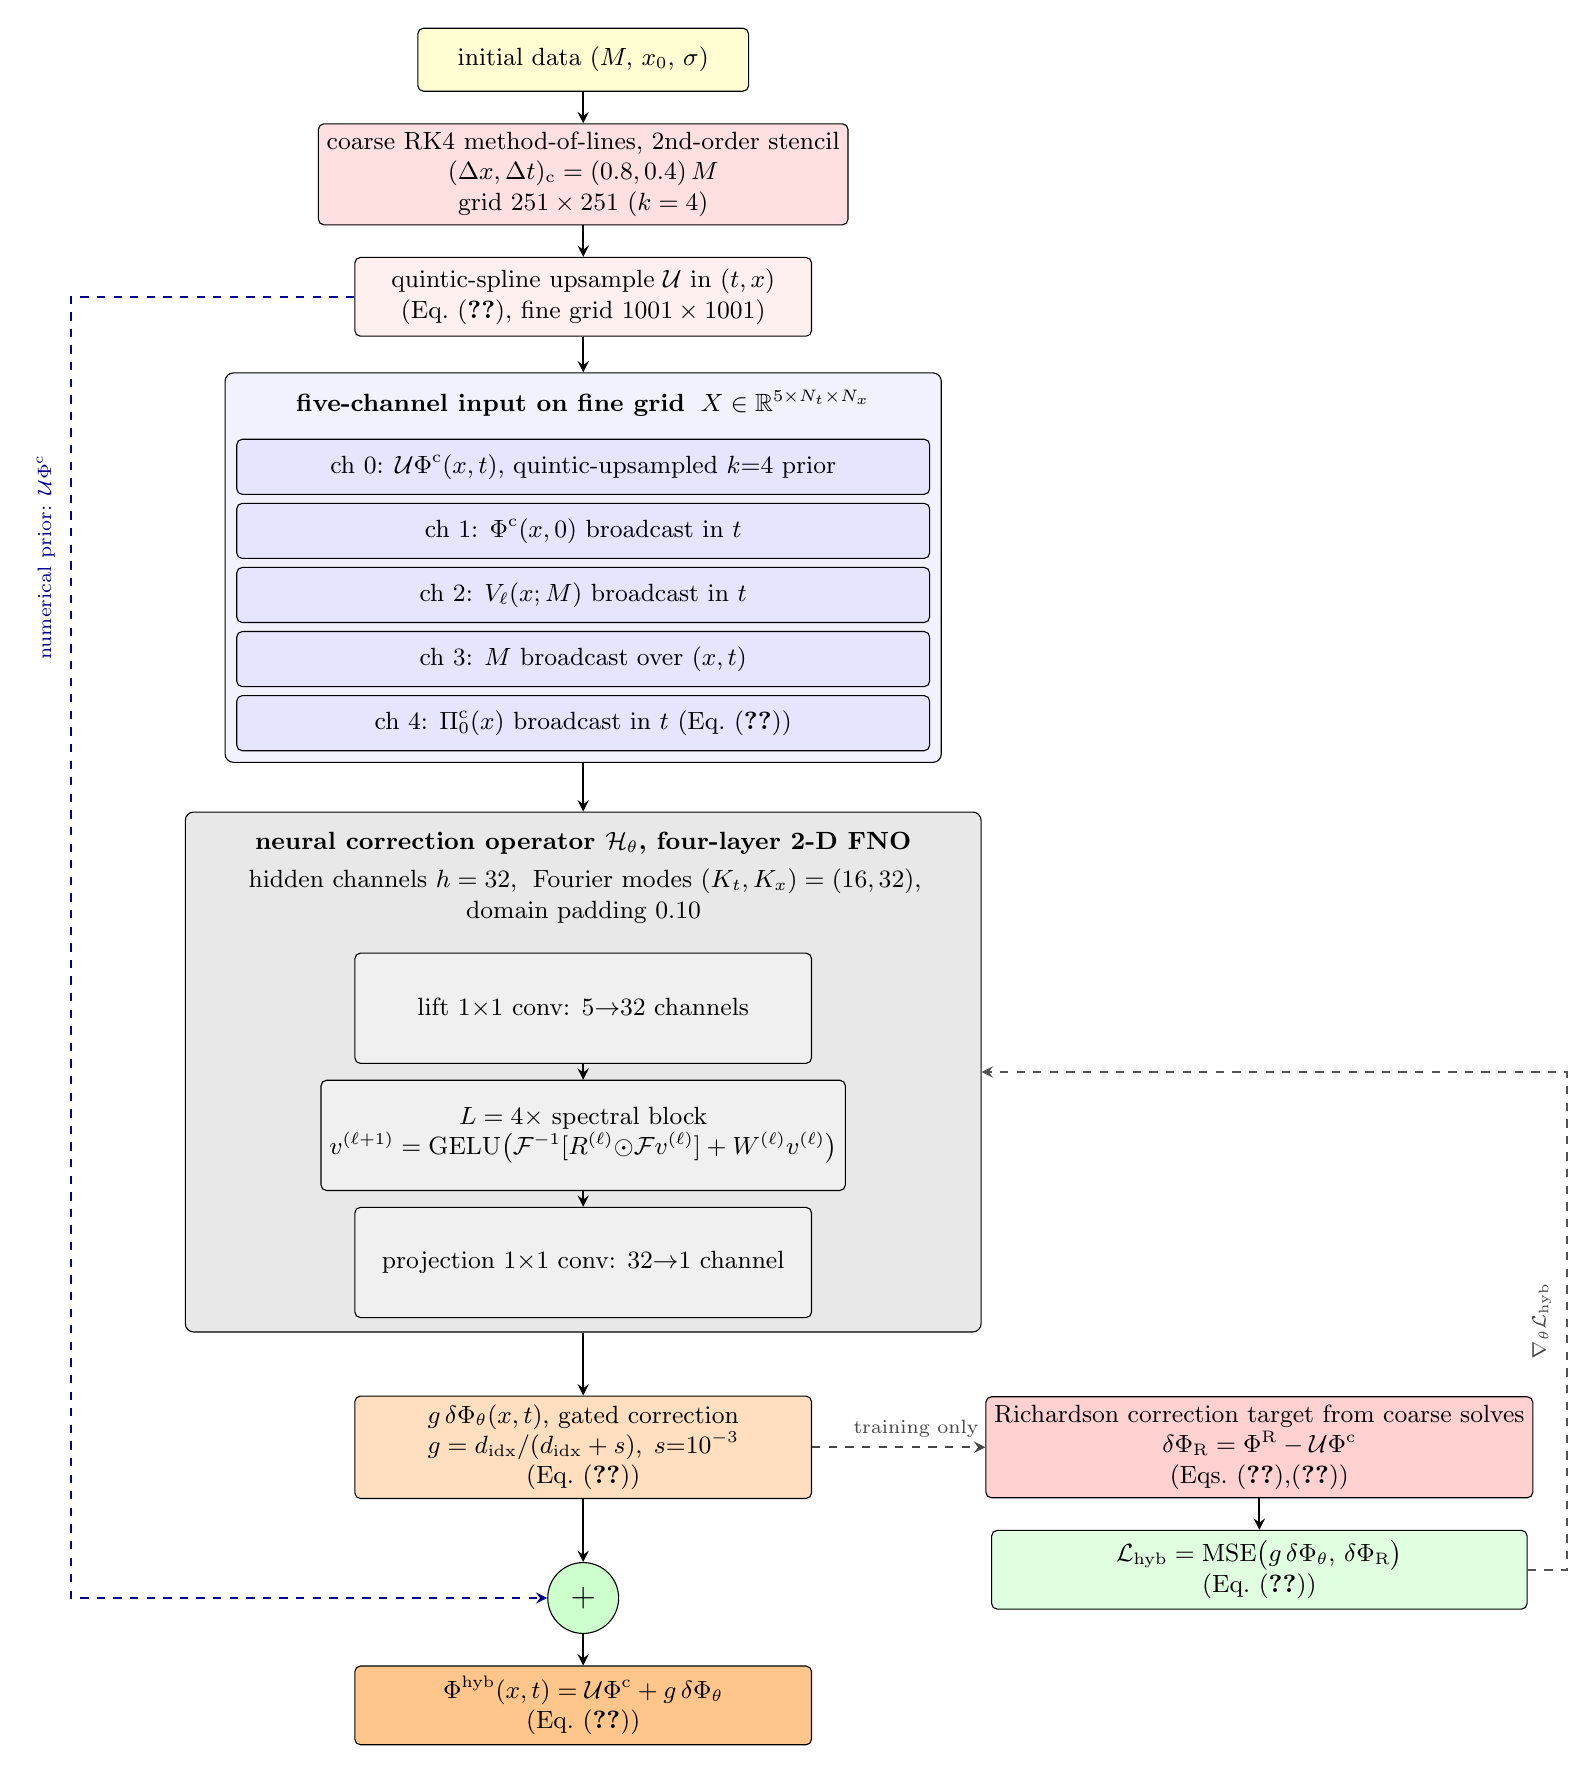
\begin{tikzpicture}[
  every node/.style={font=\small},
  ic/.style={rectangle, draw, fill=yellow!18, rounded corners=2pt,
             minimum height=8mm, minimum width=42mm, inner sep=3pt,
             align=center},
  fd/.style={rectangle, draw, fill=red!12, rounded corners=2pt,
             minimum height=11mm, minimum width=58mm, inner sep=3pt,
             align=center},
  up/.style={rectangle, draw, fill=red!6, rounded corners=2pt,
             minimum height=10mm, minimum width=58mm, inner sep=3pt,
             align=center},
  inp/.style={rectangle, draw, fill=blue!10, rounded corners=2pt,
              minimum height=7mm, minimum width=88mm, inner sep=3pt,
              align=center, font=\small},
  stack/.style={rectangle, draw=none, fill=none,
                inner sep=2pt, align=center, font=\small},
  stackbg/.style={rectangle, draw, fill=blue!5, rounded corners=3pt,
                  inner sep=4pt},
  fnobox/.style={rectangle, draw, fill=gray!12, rounded corners=2pt,
                 minimum height=14mm, minimum width=58mm, inner sep=3pt,
                 align=center},
  fnoblock/.style={rectangle, draw=none, fill=none,
                   inner sep=2pt, align=center},
  fnobg/.style={rectangle, draw, fill=gray!18, rounded corners=3pt,
                inner sep=5pt},
  outn/.style={rectangle, draw, fill=orange!25, rounded corners=2pt,
               minimum height=10mm, minimum width=58mm, inner sep=3pt,
               align=center},
  sum/.style={circle, draw, fill=green!20, inner sep=0pt,
              minimum size=9mm, font=\large},
  loss/.style={rectangle, draw, fill=green!12, rounded corners=2pt,
               minimum height=10mm, minimum width=68mm, inner sep=3pt,
               align=center},
  arr/.style={->, >=stealth, thick, black},
  arrs/.style={->, >=stealth, thick, blue!55!black, dashed},
  arrt/.style={->, >=stealth, thick, gray!55!black, dashed},
  sec/.style={font=\footnotesize\itshape, gray!55!black, anchor=west},
]
  % ============ classical solver path ============
  \node[ic]   (icbox) {initial data $(M,\,x_{0},\,\sigma)$};
  \node[fd, below=4mm of icbox]
        (cfd)   {coarse RK4 method-of-lines, 2nd-order stencil\\
                 $(\Delta x,\Delta t)_{\mathrm{c}}=(0.8,0.4)\,M$ \\
           grid $251\times 251$ ($k=4$)};
  \node[up, below=4mm of cfd]
        (upbox) {quintic-spline upsample $\mathcal{U}$ in $(t,x)$\\
           (Eq.~\eqref{eq:hyb-upsample}, fine grid $1001\times 1001$)};

  \draw[arr] (icbox) -- (cfd);
  \draw[arr] (cfd) -- (upbox);

  % ============ five-channel input stack ============
  \node[stack, below=6mm of upbox] (stackhdr) {%
    \textbf{five-channel input on fine grid}\;
    $X\in\mathbb{R}^{5\times N_{t}\times N_{x}}$};
  \node[inp, below=2mm of stackhdr]
      (c0) {ch~0: $\mathcal{U}\Phi^{\mathrm{c}}(x,t)$, quintic-upsampled $k{=}4$ prior};
  \node[inp, below=1mm of c0]
        (c1) {ch~1: $\Phi^{\mathrm{c}}(x,0)$ broadcast in $t$};
  \node[inp, below=1mm of c1]
        (c2) {ch~2: $V_{\ell}(x;M)$ broadcast in $t$};
  \node[inp, below=1mm of c2]
        (c3) {ch~3: $M$ broadcast over $(x,t)$};
  \node[inp, below=1mm of c3]
        (c4) {ch~4: $\Pi^{\mathrm{c}}_{0}(x)$ broadcast in $t$
              (Eq.~\eqref{eq:hyb-pi0})};
  \begin{scope}[on background layer]
    \node[stackbg, fit=(stackhdr)(c0)(c4)] (stackbg) {};
  \end{scope}

  \draw[arr] (upbox) -- (stackbg.north);

  % ============ FNO correction operator ============
  \node[fnoblock, below=8mm of stackbg.south] (fnohdr) {%
    \begin{minipage}{96mm}
      \centering
      \textbf{neural correction operator $\mathcal{H}_{\theta}$, four-layer 2-D FNO}\\[1mm]
      hidden channels $h=32$,\;
      Fourier modes $(K_{t},K_{x})=(16,32)$,\;
      domain padding $0.10$
    \end{minipage}};

  \node[fnobox, below=3mm of fnohdr]
        (lift)  {lift $1{\times}1$ conv: $5{\to}32$ channels};
  \node[fnobox, below=2mm of lift]
        (sb)    {$L=4 \times$ spectral block\\
                 $v^{(\ell+1)}=\mathrm{GELU}\bigl(
                  \mathcal{F}^{-1}[R^{(\ell)}{\odot}\mathcal{F}v^{(\ell)}]
                  + W^{(\ell)}v^{(\ell)}\bigr)$};
  \node[fnobox, below=2mm of sb]
        (proj)  {projection $1{\times}1$ conv: $32{\to}1$ channel};

  \draw[arr] (lift) -- (sb);
  \draw[arr] (sb) -- (proj);
  \begin{scope}[on background layer]
    \node[fnobg, fit=(fnohdr)(lift)(proj)] (fnoall) {};
  \end{scope}

  \draw[arr] (stackbg.south) -- (fnoall.north);

    % ============ output correction + reconstruction ============
  \node[outn, below=8mm of fnoall.south]
      (delta) {$g\,\delta\Phi_{\theta}(x,t)$, gated correction\\
           $g=d_{\mathrm{idx}}/(d_{\mathrm{idx}}+s),\;s{=}10^{-3}$\\
                 (Eq.~\eqref{eq:hyb-gate})};
  \draw[arr] (fnoall.south) -- (delta.north);

  % sum node and Phi_hybrid
  \node[sum, below=8mm of delta] (sumn) {$+$};
  \node[outn, fill=orange!45, below=4mm of sumn]
        (phih)  {$\Phi^{\mathrm{hyb}}(x,t)
                 =\mathcal{U}\Phi^{\mathrm{c}}+g\,\delta\Phi_{\theta}$\\
                 (Eq.~\eqref{eq:hyb-reconstruct})};
  \draw[arr] (delta) -- (sumn);
  \draw[arr] (sumn) -- (phih);

  % skip connection from upsample (long curve down the left)
  \draw[arrs] (upbox.west) -- ++(-3.6,0) |-
              node[pos=0.10, anchor=south, rotate=90, font=\scriptsize, blue!55!black, yshift=2pt]
                      {numerical prior: $\mathcal{U}\Phi^{\mathrm{c}}$}
              (sumn.west);

  % training-only target + loss (right side, dashed)
  \node[outn, fill=red!18, right=22mm of delta]
        (target){Richardson correction target from coarse solves\\
                 $\delta\Phi_{\mathrm{R}}=\Phi^{\mathrm{R}}-\mathcal{U}\Phi^{\mathrm{c}}$\\
                 (Eqs.~\eqref{eq:hyb-richardson},\eqref{eq:hyb-residual})};
  \node[loss, below=4mm of target]
        (lhyb)  {$\mathcal{L}_{\mathrm{hyb}}
                 =\mathrm{MSE}\bigl(g\,\delta\Phi_{\theta},\,\delta\Phi_{\mathrm{R}}\bigr)$\\
                 (Eq.~\eqref{eq:hyb-loss})};
  \draw[arrt] (delta.east) --
              node[pos=0.60, above, font=\scriptsize, gray!55!black] {training only}
              (target.west);
  \draw[arr]  (target) -- (lhyb);

  % gradient backflow from loss to FNO (training only)
  \draw[arrt, gray!65!black] (lhyb.east) -- ++(0.5,0) |-
              node[pos=0.25, anchor=south, rotate=90, font=\scriptsize, gray!55!black, yshift=2pt]
            {$\nabla_{\theta}\mathcal{L}_{\mathrm{hyb}}$}
              (fnoall.east);
\end{tikzpicture}
}
\caption{Schwarzschild hFNO pipeline of Sec.~\ref{sec:hyb-method}.
The classical RK4
method-of-lines solver of Appendix~\ref{app:fd} produces the
coarse field $\Phi^{\mathrm{c}}$ on
$(\Delta x,\Delta t)_{\mathrm{c}} = (0.8,0.4)\,M$ ($k=4$), which
is quintic-spline upsampled in $(t,x)$ onto the fine grid by the
operator $\mathcal{U}$ of Eq.~\eqref{eq:hyb-upsample}. The
five-channel input stack combines this prior
$\mathcal{U}\Phi^{\mathrm{c}}$ with the initial displacement
$\Phi^{\mathrm{c}}(x,0)$, initial velocity
$\Pi^{\mathrm{c}}_{0}(x)$ (Eq.~\eqref{eq:hyb-pi0}), Zerilli
potential $V_{\ell}(x;M)$ and broadcast mass $M$. A four-layer
2-D FNO $\mathcal{H}_{\theta}$ with hidden channel count
$h = 32$ and retained Fourier modes $(K_{t},K_{x}) = (16,32)$
predicts an additive correction, which is multiplied by the
deterministic fixed-scale gradient gate
$g=d_{\mathrm{idx}}/(d_{\mathrm{idx}}+s)$
(Eq.~\eqref{eq:hyb-gate}, $s = 10^{-3}$, a deterministic
function of the prior) before being added back; the hybrid
prediction Eq.~\eqref{eq:hyb-reconstruct} adds the
quintic-upsampled coarse field explicitly (blue dashed),
and the gate confines the correction to the under-resolved
wavefronts. The dashed grey path on the right depicts the
training-only Richardson correction target
$\delta\Phi_{\mathrm{R}} = \Phi^{\mathrm{R}} -
\mathcal{U}\Phi^{\mathrm{c}}$
(Eqs.~\eqref{eq:hyb-richardson},\eqref{eq:hyb-residual}), built
from $k = 4$ and $k = 2$ coarse solves alone, and the MSE loss
Eq.~\eqref{eq:hyb-loss} against which $\mathcal{H}_{\theta}$ is
fitted; at inference time the right-hand path is absent and
only the single $k = 4$ coarse solve and the left-hand
reconstruction path are evaluated. Total trainable parameters:
$1.13\times 10^{6}$.}
\label{fig:hyb-arch}
\end{figure}

\paragraph{Discretisation and grids.} The fine and coarse solves use
the same physical domain and the same RK4 method-of-lines scheme as
Appendix~\ref{app:fd}, with the same second-order centred stencil.
The fine evolution has $N_x=1001$ points and $N_{\mathrm{step}}=1000$
time steps, while the $k=4$ prior has $N_x=251$ and
$N_{\mathrm{step}}=250$. Since every RK4 stage is linear in $N_x$,
the coarse-to-fine ratio of finite-difference point updates is
\begin{equation}
  \frac{N_x^{\mathrm c}N_{\mathrm{step}}^{\mathrm c}}
       {N_x^{\mathrm f}N_{\mathrm{step}}^{\mathrm f}}
  = \frac{251\times250}{1001\times1000}
  \approx \frac{1}{16}.
  \label{eq:hyb-work-ratio}
\end{equation}

\paragraph{Richardson-extrapolated field and correction target.} For the second-order
stencil, the leading coarse-grid error is
$\mathcal{O}(\Delta x_{\mathrm{c}}^2)$. We upsample the $k=4$ and
$k=2$ fields with $\mathcal{U}$ and form the Richardson-extrapolated field in
Eq.~\eqref{eq:hyb-richardson}.
\begin{equation}
  \Phi^{\mathrm{R}}
  \;=\; \frac{4\,\mathcal{U}\Phi^{\mathrm{c}}_{2}
              - \mathcal{U}\Phi^{\mathrm{c}}}{3},
  \label{eq:hyb-richardson}
\end{equation}
This cancels the leading error, giving
$\Phi^{\mathrm{R}}=\Phi+\mathcal{O}(\Delta x_{\mathrm{c}}^4)$ up to
interpolation error. The correction target is
\begin{equation}
  \delta\Phi_{\mathrm{R}}(x, t)
  \;=\; \Phi^{\mathrm{R}}(x, t) - \mathcal{U}\Phi^{\mathrm{c}}(x, t),
  \label{eq:hyb-residual}
\end{equation}
and agrees with the true coarse-grid error up to the remaining
fourth-order Richardson and interpolation errors. It is obtained
entirely from coarse solves. The fine reference field is used only for
evaluation, while inference requires only the $k=4$ solve. The target
is concentrated on under-resolved wavefronts, motivating the gate in
Eq.~\eqref{eq:hyb-gate}.

\paragraph{Upsample operator.} The operator $\mathcal{U}$ is the
degree-five tensor-product spline
\begin{equation}
  (\mathcal{U}\Phi^{\mathrm{c}})(x, t)
  \;=\; \sum_{i, j} c_{ij}\,
        B_{5}\!\Bigl(\tfrac{t - t_{i}}{\Delta t_{\mathrm{c}}}\Bigr)\,
        B_{5}\!\Bigl(\tfrac{x - x_{j}}{\Delta x_{\mathrm{c}}}\Bigr),
  \label{eq:hyb-upsample}
\end{equation}
Here $B_5$ is the quintic B-spline basis and the coefficients
interpolate the coarse nodes. The same operator is applied to both
coarse fields. For smooth data, its formal order exceeds the
fourth-order Richardson remainder, and its interpolation error is
smaller than the correction target in the tested regime.

\paragraph{Input stack.} The input contains the upsampled prior,
initial displacement, Zerilli potential, broadcast mass and the
initial velocity estimate
\begin{equation}
  \Pi^{\mathrm{c}}_{0}(x)
  \;=\; \frac{\Phi^{\mathrm{c}}(x, \Delta t_{\mathrm{c}}) -
              \Phi^{\mathrm{c}}(x, 0)}{\Delta t_{\mathrm{c}}},
  \label{eq:hyb-pi0}
\end{equation}
computed on the coarse grid and linearly resampled to the fine $x$
grid. The velocity is an auxiliary input rather than a supervised
target. The prior channel supplies the coarse evolution.
The parameters $x_0$ and $\sigma$ are encoded by the initial
displacement and velocity fields, while $M$ is supplied explicitly
and through the potential. Thus $X$ identifies both the initial-value
problem and the spatial operator whose discretisation error is being
corrected.

\paragraph{Correction operator, gradient gate, and reconstruction.}
The neural correction operator
\begin{equation}
  \mathcal{H}_{\theta}\colon\;
  X = \bigl[\mathcal{U}\Phi^{\mathrm{c}},\,\Phi^{\mathrm{c}}(\cdot, 0),\,
            V_{\ell}(\cdot; M),\,M,\,\Pi^{\mathrm{c}}_{0}\bigr]
  \;\longmapsto\;
  \delta\Phi_{\theta}(x, t)
  \label{eq:hyb-operator}
\end{equation}
is modulated by a deterministic fixed-scale gradient gate before it is
added to the prior. For $P_{ij}=P(x_j,t_i)$, the implementation forms
the index-space gradient magnitude
\begin{equation}
  d_{\mathrm{idx},ij}
  = \sqrt{(\Delta_i P_{ij})^2+(\Delta_j P_{ij})^2},
  \qquad
  g_{ij}=\frac{d_{\mathrm{idx},ij}}{d_{\mathrm{idx},ij}+s},
  \label{eq:hyb-gate}
\end{equation}
where $\Delta_i$ and $\Delta_j$ are the finite differences returned
with unit grid-index spacing. On the fixed $1001\times1001$ grid, we
set $s=Q_{0.68}(d_{\mathrm{idx}})=10^{-3}$ using only the deployment
prior. The gate is a deterministic function of the prior alone. It
approaches one on wavefronts with large
$d_{\mathrm{idx}}$, where the numerical prior has its largest
dispersion error, and
zero in smooth regions away
from the wavefronts, including the numerically zero region ahead of
the outgoing signal. The corrected field is reconstructed by adding
the gated FNO correction to the interpolated coarse solution,
\begin{equation}
  \Phi^{\mathrm{hyb}}(x, t)
  \;=\; \mathcal{U}\Phi^{\mathrm{c}}(x, t)
         + g(x, t)\,\mathcal{H}_{\theta}(X)(x, t),
  \label{eq:hyb-reconstruct}
\end{equation}
which confines the correction to the under-resolved regions by
construction and reduces to the quintic-upsampled coarse solve
(the upsampled numerical prior of Sec.~\ref{sec:res-hyb}) wherever
$g = 0$ or $\mathcal{H}_{\theta} \equiv 0$.

\paragraph{FNO architecture.} The correction operator
$\mathcal{H}_{\theta}$ is a 2-D Fourier neural operator
\citep{Li2021fno,Kovachki2023neuralop} on the fine $(t, x)$
grid: a $1\times 1$ lift to $h = 32$ hidden channels, $L = 4$
Fourier layers of the form
\begin{equation}
  v^{(\ell+1)}(x, t)
  \;=\; \mathrm{GELU}\!\Bigl(
         \mathcal{F}^{-1}\bigl[R^{(\ell)} \odot
         \mathcal{F}\,v^{(\ell)}\bigr](x, t)
         \;+\; W^{(\ell)}\,v^{(\ell)}(x, t)
       \Bigr),
  \label{eq:hyb-fno-layer}
\end{equation}
and a $1\times 1$ projection back to one channel, where
$\mathcal{F}$ is the 2-D DFT along $(t, x)$, $R^{(\ell)}$ the
complex spectral-weight tensor truncated to
$(K_{t}, K_{x}) = (16, 32)$ retained modes (matching the $2{:}1$
spatial-to-temporal domain-length ratio and resolving
$k_{x} \lesssim 1.0\,M^{-1}$), $\odot$ mode-by-mode matrix
multiplication across channels, and $W^{(\ell)}$ a pointwise
linear path. Each axis is pre-padded by $p = 0.10$ against
periodic wraparound, and positional $(x, t)$ encodings break
translation equivariance to distinguish the source region from
the wave zones. The total parameter count is $1.13\times 10^{6}$ under the
\texttt{neuraloperator} implementation \citep{Kovachki2023neuralop}.
The lift first maps the five physical inputs to $h$ feature fields.
Within each layer, the Fourier path couples retained modes and feature
channels globally over the complete space-time domain, while
$W^{(\ell)}$ supplies a local pointwise update. The inverse transform
returns the global update to physical space, GELU combines the two
paths nonlinearly, and the final projection returns one correction
field. The smaller width is used because the FNO predicts a
correction rather than the full field.

\paragraph{Loss.} The training loss is the gridwise mean
squared error between the gated network output and the
Richardson correction target built from coarse solves,
\begin{equation}
  \mathcal{L}_{\mathrm{hyb}}(\theta)
  \;=\; \frac{1}{B}\sum_{b=1}^{B}
         \frac{1}{N_{t} N_{x}}
         \sum_{i=1}^{N_{t}}\sum_{j=1}^{N_{x}}
         \bigl[
           g^{(b)}_{ij}\,\mathcal{H}_{\theta}(X^{(b)})_{ij}
           \,-\, \delta\Phi^{(b)}_{\mathrm{R},\,ij}
         \bigr]^{2},
  \label{eq:hyb-loss}
\end{equation}
Because the gate is part of the forward map, the loss trains the
correction after gating rather than the raw FNO output. No auxiliary,
spatially weighted or sample-normalisation terms are used.

\paragraph{Optimiser.} The hFNO is trained with AdamW for $100$ epochs
using the settings in Table~\ref{tab:train-config}. The checkpoint
with the lowest validation MSE is used for evaluation.

\paragraph{Training data.} The Sobol parameter ranges, dataset sizes
and canonical configuration are listed in
Table~\ref{tab:surrogate-config}. The fine, $k = 4$ and $k = 2$
solves are precomputed and cached for the same Sobol triples, so each
Richardson pair represents one initial-value problem. The ranges of
$x_0$ and $\sigma$ keep the prompt burst within the simulation window
for all sampled configurations.

% --------------------------------------------------------------
\subsection{Kerr radial Teukolsky evolution}
\label{sec:teukolsky-numerics}

The Kerr calculation uses a $1+1$ radial model for the $(4,2,0)$ mode
derived from the spin-weight $s=-2$ Teukolsky equation in minimal-gauge
horizon-penetrating hyperboloidal coordinates
\citep{Zenginoglu2011,Harms2013,PanossoMacedo2020}. The compactified
radial coordinate is
\begin{equation}
  \sigma = \frac{r_{+}}{r} \in [0, 1],
  \qquad
  \sigma = 1 \ \text{(horizon)}, \quad
  \sigma = 0 \ (\scri),
  \label{eq:kerr-sigma}
\end{equation}
The time coordinate is replaced by a hyperboloidal time $\tau$ whose
constant-time slices connect the horizon to $\scri$
(Fig.~\ref{fig:kerr-slicing}). On this slice the radial
characteristics leave the domain at both endpoints, into the horizon
and through $\scri$. The evolution is therefore fixed by regular
initial data, with no external boundary data imposed
\citep{Harms2013,PanossoMacedo2020}. To keep the evolved field finite
at both endpoints we use
\begin{equation}
  \Psi = \psi\,\sigma^{3}\,(1 - \sigma)^{-2 - i\beta},
  \qquad
  \beta = \frac{m a}{r_{+} - r_{-}},
  \label{eq:kerr-rescale}
\end{equation}
where $\sigma^3$ accounts for the asymptotic peeling at $\scri$, while
$(1-\sigma)^{-2-i\beta}$ regularises the horizon behaviour. The phase
$\beta = ma/(r_+-r_-)$ carries the spin-dependent azimuthal
frame-dragging contribution.

\begin{figure}[!htbp]
\centering
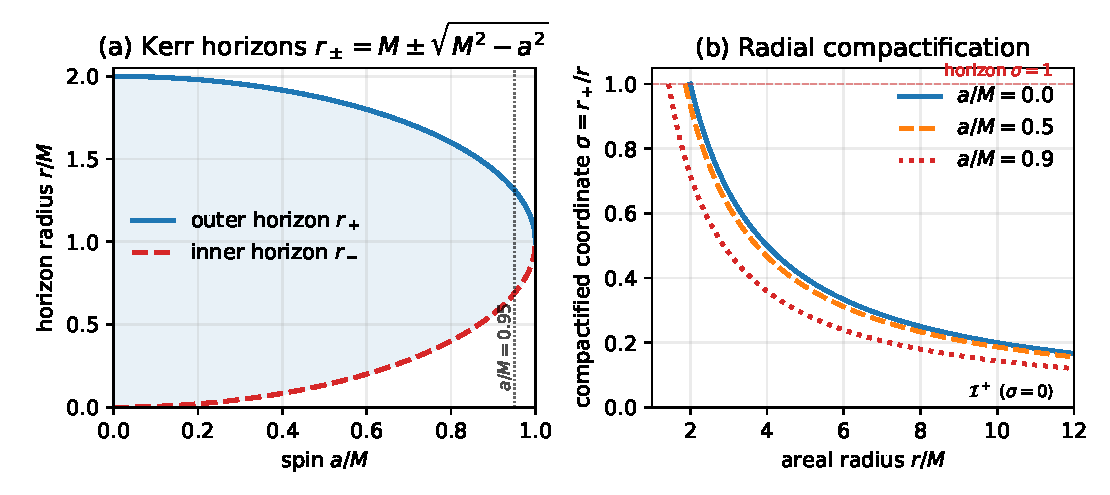
\includegraphics[width=0.92\textwidth]{../outputs/background/kerr_horizons.pdf}
\caption{Kerr geometry and radial coordinate. (a) The outer and
inner horizons $r_{\pm} = M \pm \sqrt{M^{2}-a^{2}}$
(Eq.~\eqref{eq:kerr-horizons}) as functions of spin; they
coincide at extremality $a = M$, and the study range reaches
$a/M = 0.95$ (dotted). (b) The compactification
$\sigma = r_{+}/r$ of Eq.~\eqref{eq:kerr-sigma} for three spins,
mapping the exterior $r \in [r_{+}, \infty)$ onto
$\sigma \in [0, 1]$ with the horizon at $\sigma = 1$ and future
null infinity $\scri$ at $\sigma = 0$. It replaces the finite
tortoise-grid description used for the Schwarzschild calculation.}
\label{fig:kerr-coords}
\end{figure}

\begin{figure}[!htbp]
\centering
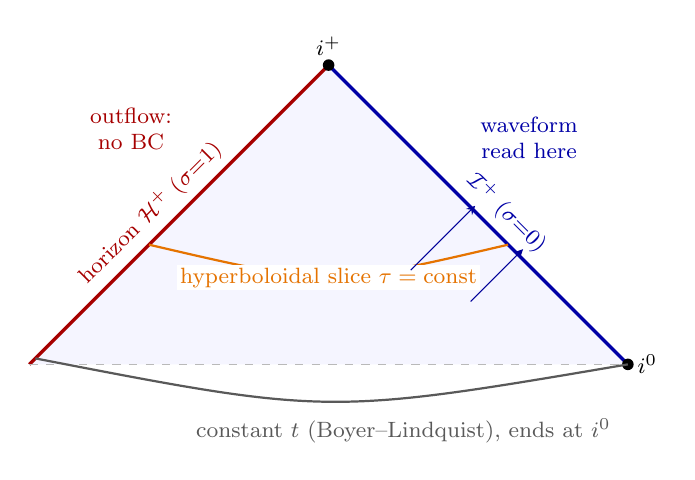
\begin{tikzpicture}[scale=1.9, >=stealth,
                    every node/.style={font=\footnotesize}]
  \coordinate (B)  at (0,0);
  \coordinate (i0) at (4,0);
  \coordinate (ip) at (2,2);
  \fill[blue!4] (B) -- (i0) -- (ip) -- cycle;
  % future horizon (sigma=1) and null infinity (sigma=0)
  \draw[very thick, red!65!black]  (B)  -- (ip);
  \draw[very thick, blue!65!black] (i0) -- (ip);
  \draw[gray!55, dashed] (B) -- (i0);
  \fill (i0) circle (1.1pt);  \fill (ip) circle (1.1pt);
  \node[right]      at (i0) {$i^{0}$};
  \node[above]      at (ip) {$i^{+}$};
  \node[red!65!black, rotate=45, anchor=south, xshift=-3pt]
       at (0.95,0.95) {horizon $\mathcal{H}^{+}\ (\sigma{=}1)$};
  \node[blue!65!black, rotate=-45, anchor=south, xshift=3pt]
       at (3.05,0.95) {$\scri\ (\sigma{=}0)$};
  % Boyer-Lindquist constant-t slice: ends at i^0
  \draw[thick, gray!70!black] (0.04,0.04) .. controls (2,-0.34) .. (i0);
  \node[gray!70!black, below, align=center] at (2.5,-0.30)
       {constant $t$ (Boyer--Lindquist),\ ends at $i^{0}$};
  % hyperboloidal slice: horizon -> scri
  \draw[thick, orange!90!black]
       (0.80,0.80) .. controls (2,0.52) .. (3.20,0.80);
  \node[orange!90!black, fill=white, inner sep=1pt, align=center]
       at (2.0,0.58) {hyperboloidal slice $\tau=\mathrm{const}$};
  % outgoing radiation (slope +1) reaching scri
  \draw[->, blue!60!black] (2.55,0.63) -- (2.98,1.06);
  \draw[->, blue!60!black] (2.95,0.42) -- (3.30,0.77);
  % annotations
  \node[red!65!black,  align=center, anchor=north] at (0.68,1.78)
       {outflow:\\ no BC};
  \node[blue!65!black, align=center, anchor=north] at (3.34,1.72)
       {waveform\\ read here};
\end{tikzpicture}
\caption{Conformal (Penrose) diagram of the Kerr exterior in the
hyperboloidal minimal gauge. The exterior is bounded by the
future horizon $\mathcal{H}^{+}$ ($\sigma = 1$, red) and future
null infinity $\scri$ ($\sigma = 0$, blue), meeting at future
timelike infinity $i^{+}$. A Boyer--Lindquist constant-$t$ slice
(grey) approaches spatial infinity $i^{0}$, whereas a hyperboloidal
slice $\tau = \mathrm{const}$ (orange) reaches future null infinity.
The outgoing ringdown (blue arrows) is captured at $\scri$. Both
endpoints are outflow boundaries, so no boundary data are imposed.}
\label{fig:kerr-slicing}
\end{figure}

\paragraph{Radial Teukolsky evolution for the $(4,2,0)$ mode.} For
each spin, the angular sector is fixed at the spheroidal eigenvalue
${}_{-2}A_{42}(a\omega_{\mathrm{ref}})$ evaluated at the
spin-dependent Leaver frequency of the fundamental mode. The resulting
separation constant defines a $1+1$ radial evolution in
$(\tau,\sigma)$; it is not the generic $2+1$ time-domain Teukolsky
initial-value problem \citep{Harms2013,PanossoMacedo2020}. We
integrate the radial equation with a fourth-order Runge--Kutta method
of lines and Kreiss--Oliger dissipation. Leaver's continued-fraction
values are obtained through the \texttt{qnm} package
\citep{Leaver1985,Stein2019qnm}. Because the target frequency enters
the separation constant, the fitted Kerr QNM values are compared
against Leaver but are not independent spectral predictions. The
radial field is the Kerr reference solution used for the hFNO field
errors.
The choice $\ell=4$ rather than $\ell=2$ is deliberate. Its
shorter-wavelength perturbation provides a more stringent test of
spatial under-resolution and of the hFNO's ability to recover the
corresponding wavefront structure (Fig.~\ref{fig:kerr-spectrum}a).

The $N=201$ and $N=401$ fields do not use the $N=801$ reference.

\begin{table}[!htbp]
\centering
\caption{Kerr dataset and numerical configuration.}
\label{tab:kerr-numerics}
\footnotesize
\setlength{\tabcolsep}{5pt}
\begin{tabular}{@{}ll@{}}
\toprule
Property & Value \\
\midrule
Radial model and target mode & $s=-2$, $(\ell,m,n)=(4,2,0)$, $M=1$ \\
Domain and readout & $\sigma\in[0,1]$, $\tau/M\in[0,220]$, $\scri$ at $\sigma=0$ \\
Initial data & $\Psi(0,r)=\exp[-(r-r_0)^2/(2w^2)]$, $\partial_\tau\Psi(0,r)=0$ \\
Parameter ranges & $a/M\in[0,0.95]$, $r_0/M\in[8,11]$, $w/M\in[1,1.5]$ \\
Fine reference field & $N=801$, fourth-order centred differences \\
Richardson pair & $N=401,201$, fourth-order centred differences \\
Deployment prior & $N=101$, second-order centred differences \\
Time integration & RK4, CFL safety $0.4$, stored every $0.25\,M$ \\
Dissipation & KO strength $0.2$, matched fourth- or sixth-difference operator \\
Training/validation/test samples & Sobol seed $0$, $1024/128/128$ \\
Training seed & $1234$ \\
\bottomrule
\end{tabular}
\end{table}

QNM extraction is reported for the hFNO and fine reference fields.
The $N=101$ field is the numerical prior and field-accuracy baseline.
QNM extraction is not reported separately for it.

% --------------------------------------------------------------
\subsection{The Kerr hFNO}
\label{sec:kerr-method}

The Kerr hFNO extends the Schwarzschild correction operator of
Sec.~\ref{sec:hyb-method} to the complex Teukolsky field. For each
$q_{\mathrm K}=(a/M,r_0,w)$, the deployment prior is the full
$N=101$ field upsampled along the compactified radial direction,
\begin{equation}
  P_{\mathrm K}(q_{\mathrm K})
  =\mathcal U_\sigma\Psi_{101}^{\mathrm c}(q_{\mathrm K}).
  \label{eq:kerr-prior}
\end{equation}
All resolutions share the same stored $\tau$ grid, so no temporal
interpolation is required.

The Richardson-extrapolated field is constructed from independently
evolved $N=401$ and $N=201$ fields. Both are computed with
fourth-order spatial differences and form an exact $2{:}1$ refinement
pair, giving
\begin{equation}
  u^{\star} = \frac{16\, u_{401} - u_{201}}{15},
  \label{eq:kerr-richardson}
\end{equation}
where $u_{401}$ and $u_{201}$ denote the $N = 401$ and $N = 201$
fields after spatial upsampling to the fine $\sigma$ grid. This
cancels the leading $\mathcal O(\Delta\sigma^4)$ spatial error. The
different Richardson coefficients in Eqs.~\eqref{eq:hyb-richardson}
and~\eqref{eq:kerr-richardson} follow directly from the second-order
Schwarzschild and fourth-order Kerr stencils. The $N=101$ deployment
prior is deliberately separate from this finer target pair. It
retains a cheap inference solve while the two finer fields are
needed only during training.

The field amplitude varies substantially across the parameter family.
Each sample is therefore scaled by the RMS magnitude of its prior,
\begin{equation}
  s_b
  =\left[
      \frac{1}{N_\tau N_\sigma}
      \sum_{i=1}^{N_\tau}\sum_{j=1}^{N_\sigma}
      |P_{\mathrm K}^{(b)}(\tau_i,\sigma_j)|^2
    \right]^{1/2}.
  \label{eq:kerr-scale}
\end{equation}
This scale depends only on the deployment prior and is available at
inference. The four input channels and the normalised target are
\begin{align}
  X_{\mathrm K}^{(b)}
  &=\left[
      \frac{\operatorname{Re}P_{\mathrm K}^{(b)}}{s_b},
      \frac{\operatorname{Im}P_{\mathrm K}^{(b)}}{s_b},
      \frac{a_b}{M},
      \frac{\operatorname{Re}P_{\mathrm K}^{(b)}(0,\cdot)}{s_b}
    \right],
  \nonumber\\
  Y_{\mathrm K}^{(b)}
  &=\left[
      \frac{\operatorname{Re}(u_b^\star-P_{\mathrm K}^{(b)})}{s_b},
      \frac{\operatorname{Im}(u_b^\star-P_{\mathrm K}^{(b)})}{s_b}
    \right].
  \label{eq:kerr-input-target}
\end{align}
The spin channel and initial pulse specify the configuration, while
the real and imaginary prior channels provide the reduced-resolution
evolution.

The FNO returns two normalised correction channels. Writing these as
$\mathcal H_{\theta,1}$ and $\mathcal H_{\theta,2}$, the physical
field is reconstructed by
\begin{equation}
  \Psi^{\mathrm{hyb}}_b
  =P_{\mathrm K}^{(b)}
   +s_b\left[
      \mathcal H_{\theta,1}(X_{\mathrm K}^{(b)})
      +\mathrm i\,\mathcal H_{\theta,2}(X_{\mathrm K}^{(b)})
    \right].
  \label{eq:kerr-reconstruct}
\end{equation}
The training objective is the uniform MSE over both correction
channels,
\begin{equation}
  \mathcal L_{\mathrm K}(\theta)
  =\frac{1}{2BN_\tau N_\sigma}
   \sum_{b=1}^{B}\sum_{c=1}^{2}
   \sum_{i=1}^{N_\tau}\sum_{j=1}^{N_\sigma}
   \left[
     \mathcal H_{\theta,c}(X_{\mathrm K}^{(b)})_{ij}
     -Y_{\mathrm K,c,ij}^{(b)}
   \right]^2.
  \label{eq:kerr-loss}
\end{equation}
No $N=801$ field enters this loss. Those fields are used only to
evaluate the hFNO after reconstruction.

The correction operator has four Fourier layers, width $48$, retained
modes $(K_\tau,K_\sigma)=(64,24)$, grid positional encodings and
padding $(0.08,0.08)$. The greater number of temporal modes resolves
the oscillatory ringdown, while the compactified radial dependence is
smoother. The network contains $7{,}697{,}042$ trainable parameters
and is trained in single precision with Adam, an initial learning
rate of $10^{-3}$, weight decay $10^{-6}$ and batch size $8$. A
cosine schedule reduces the learning rate over at most $200$ epochs.
Training stops after $30$ epochs without validation improvement, and
the checkpoint with the lowest validation MSE is used for evaluation.

Unlike the Schwarzschild construction, the Kerr correction is not
multiplied by a gradient gate. Unlike the Schwarzschild field, the
hyperboloidal field is nonzero over nearly the entire domain, and
phase and damping errors at $\scri$ persist into the low-amplitude
ringdown. A prior-gradient gate would
therefore suppress corrections where the QNM signal is measured. At
inference, Eqs.~\eqref{eq:kerr-prior}
and~\eqref{eq:kerr-reconstruct} require one $N=101$ solve and one FNO
evaluation; the Richardson pair and fine reference field are absent.
Figure~\ref{fig:kerr-arch} shows the training and inference paths.

\begin{figure}[!htbp]
\centering
\resizebox{0.82\textwidth}{!}{%
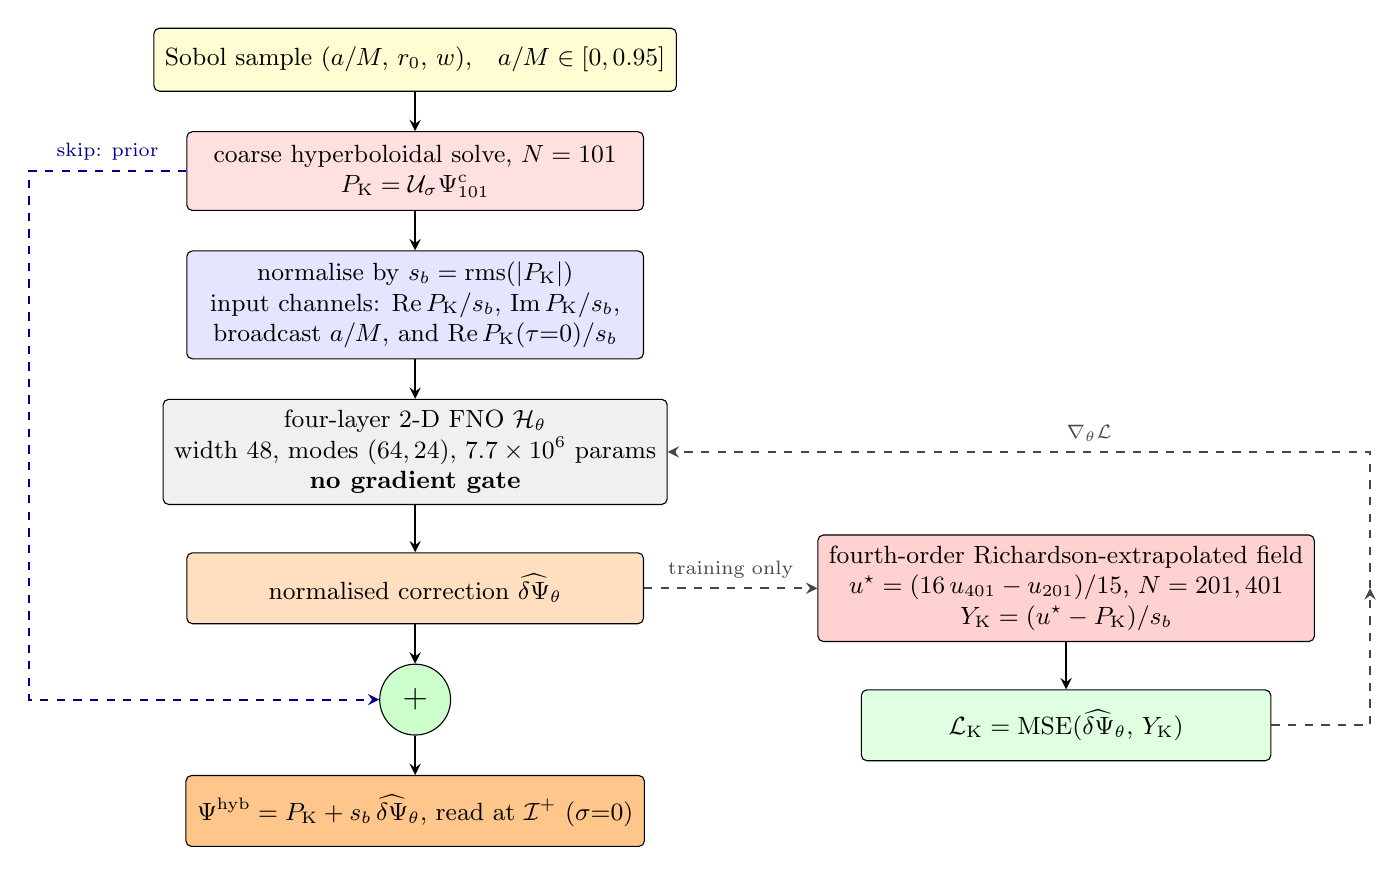
\begin{tikzpicture}[
  every node/.style={font=\small},
  box/.style={rectangle, draw, rounded corners=2pt,
              inner sep=4pt, align=center},
  ic/.style={box, fill=yellow!18, minimum height=8mm, minimum width=54mm},
  solve/.style={box, fill=red!12, minimum height=10mm, minimum width=58mm},
  inp/.style={box, fill=blue!10, minimum height=9mm, minimum width=58mm},
  fno/.style={box, fill=gray!12, minimum height=12mm, minimum width=58mm},
  outn/.style={box, fill=orange!25, minimum height=9mm, minimum width=58mm},
  tgt/.style={box, fill=red!18, minimum height=9mm, minimum width=52mm},
  loss/.style={box, fill=green!12, minimum height=9mm, minimum width=52mm},
  sum/.style={circle, draw, fill=green!20, inner sep=0pt,
              minimum size=9mm, font=\large},
  arr/.style={->, >=stealth, thick, black},
  arrs/.style={->, >=stealth, thick, blue!55!black, dashed},
  arrt/.style={->, >=stealth, thick, gray!55!black, dashed},
]
  % ===== main vertical column =====
    \node[ic] (ic) {Sobol sample $(a/M,\,r_0,\,w)$,\quad $a/M\in[0,0.95]$};
  \node[solve, below=5mm of ic] (c101)
       {coarse hyperboloidal solve, $N = 101$\\
        $P_{\mathrm K}=\mathcal U_\sigma\Psi_{101}^{\mathrm c}$};
  \node[inp, below=5mm of c101] (chan)
      {normalise by $s_b=\mathrm{rms}(|P_{\mathrm K}|)$\\
       input channels: $\mathrm{Re}\,P_{\mathrm K}/s_b$, $\mathrm{Im}\,P_{\mathrm K}/s_b$,\\
       broadcast $a/M$, and $\mathrm{Re}\,P_{\mathrm K}(\tau{=}0)/s_b$};
  \node[fno, below=5mm of chan] (fno)
     {four-layer 2-D FNO $\mathcal{H}_{\theta}$\\
      width $48$, modes $(64,24)$,
      $7.7\times 10^{6}$ params\\
      \textbf{no gradient gate}};
    \node[outn, below=6mm of fno] (res)
      {normalised correction $\widehat{\delta\Psi}_{\theta}$};
  \node[sum, below=5mm of res] (sum) {$+$};
  \node[outn, fill=orange!45, below=5mm of sum] (hyb)
      {$\Psi^{\mathrm{hyb}} = P_{\mathrm K} + s_b\,\widehat{\delta\Psi}_{\theta}$,\
        read at $\scri$ ($\sigma{=}0$)};
  \draw[arr] (ic) -- (c101);
  \draw[arr] (c101) -- (chan);
  \draw[arr] (chan) -- (fno);
  \draw[arr] (fno) -- (res);
  \draw[arr] (res) -- (sum);
  \draw[arr] (sum) -- (hyb);
  % skip connection down the left (blue dashed), as in the Schwarzschild
  % hybrid pipeline of Fig.~\ref{fig:hyb-arch}
  \draw[arrs] (c101.west) -- ++(-2.0,0)
        node[pos=0.5, above, font=\scriptsize, blue!55!black]{skip: prior}
        |- (sum.west);
    % ===== training-only path (right); target level-aligned with correction =====
  \node[tgt, right=22mm of res] (tgt)
      {fourth-order Richardson-extrapolated field\\
        $u^{\star} = (16\,u_{401} - u_{201})/15$,\
       $N = 201, 401$\\
        $Y_{\mathrm K} = (u^{\star} - P_{\mathrm K})/s_b$};
  \node[loss, below=6mm of tgt] (lo)
       {$\mathcal{L}_{\mathrm K} = \mathrm{MSE}
        (\widehat{\delta\Psi}_{\theta},\,Y_{\mathrm K})$};
  \draw[arrt] (res.east) --
        node[pos=0.5, above, font=\scriptsize]{training only} (tgt.west);
  \draw[arr] (tgt) -- (lo);
  % gradient backflow (training only), routed clear to the right of the target box
  \coordinate (gback) at ([xshift=7mm]tgt.east);
  \draw[arrt] (lo.east) -| (gback);
  \draw[arrt] (gback) |- (fno.east)
        node[pos=0.7, above, font=\scriptsize]{$\nabla_{\theta}\mathcal{L}$};
\end{tikzpicture}}
\caption{Kerr hFNO pipeline of Sec.~\ref{sec:kerr-method}.
The deployment path uses a single $N = 101$ hyperboloidal solve to
produce the complex prior $P_{\mathrm K}$, which is upsampled to
the fine $\sigma$ grid and normalised by the prior-derived scale
$s_b$. The FNO receives the real and imaginary parts of the prior, the
broadcast spin $a/M$, and the initial real pulse. It predicts a
two-channel correction that is multiplied by $s_b$ and added to the
prior to give $\Psi^{\mathrm{hyb}}$ at $\scri$. The training-only path
uses the $N = 201$ and $N = 401$ solves to form the fourth-order
Richardson-extrapolated field $u^\star$ and hence the normalised
correction target $Y_{\mathrm K}$, against which
$\mathcal{H}_{\theta}$ is fitted by
Eq.~\eqref{eq:kerr-loss}. The fine reference field is used only for evaluation.
At inference the right-hand path is absent.}
\label{fig:kerr-arch}
\end{figure}

% --------------------------------------------------------------
\subsection{QNM extraction methods}
\label{sec:qnm-methods}

QNM parameters $(\omega,\tau)$ are extracted from the Schwarzschild
waveform at the fixed code coordinate $\xq=10$ and the Kerr waveform
at $\scri$. Between the
prompt response and late-time tail, a real signal is modelled as a
sum of damped sinusoids,
\begin{equation}
  \Phi(\xq, t) \;\approx\;
  \sum_{n} A_n\,\mathrm{e}^{-(t-t_0)/\tau_n}
  \cos\bigl(\omega_n(t-t_0) + \phi_n\bigr).
  \label{eq:qnm-template}
\end{equation}
The estimators are applied separately rather than sequentially. M1
and M2 reproduce the procedures of \citet{Patel2024pinn}; M3 supplies
a subspace estimate; and M4 and M5 test fit-window sensitivity with a
two-mode model. For Kerr, the real-valued methods are applied to both
field components, while c$\Phi$ and cES use the complex field. Each
method returns a candidate $(\widehat\omega,\widehat\tau)$; the
protocols below specify the windows, mode identification and
aggregation used for each geometry.

\subsubsection{Schwarzschild estimators and fit-window protocol}
\label{sec:plateau}

\paragraph{Fixed-window Schwarzschild estimators.} M1 estimates the
damping time from the logarithmic envelope at waveform extrema and
the frequency from the positive spectral maximum, following
\citet{Patel2024pinn}. The implementation applies a Hann taper, zero
padding and three-bin parabolic peak refinement. At the local maxima
$t_k$ of $|\Phi|$,
\begin{equation}
  \log|\Phi(\xq, t_k)| \;\approx\;
  \log A_{0} - \frac{t_k - t_0}{\tau_{0}},
  \label{eq:logline}
\end{equation}
so $\widehat\tau_{\mathrm{M1}}$ is minus the reciprocal of the OLS
slope. M2 instead fits the single-mode model directly,
\begin{equation}
  (\widehat A,\widehat\omega,\widehat\tau,\widehat\phi)_{\mathrm{M2}}
  =\underset{A,\,\omega>0,\,\tau>0,\,\phi}{\arg\min}
  \sum_{t_j\in W}
  \left[\Phi(\xq,t_j)-A e^{-t_j/\tau}
  \cos(\omega t_j+\phi)\right]^2,
  \label{eq:m2-fit}
\end{equation}
initialized by M1.

M3 applies ESPRIT \citep{Roy1989esprit} to the uniformly sampled
analytic signal $s_j=\Phi_j+i\mathcal H[\Phi]_j$, modelled as
\begin{equation}
  s_k
  \;\approx\; \sum_{n=0}^{K-1} c_{n}\, z_{n}^{\,k},
  \qquad
  z_{n} \;=\; e^{(-1/\tau_{n} + \mathrm{i}\omega_{n})\Delta t}.
  \label{eq:esprit-model}
\end{equation}
If $U_K$ contains the leading $K$ left singular vectors of the
Hankel matrix $H_{ij}=s_{i+j}$, the poles are the eigenvalues
\begin{equation}
  \{z_n\}_{n=0}^{K-1}
  =\operatorname{eig}\!\left[
  (U_K^{\uparrow})^{+}U_K^{\downarrow}\right],
  \qquad
  \widehat\omega_n=\frac{\operatorname{Im}\log z_n}{\Delta t},
  \qquad
  \widehat\tau_n=-\frac{\Delta t}{\operatorname{Re}\log z_n}.
  \label{eq:esprit-poles}
\end{equation}
Here $+$ denotes the Moore--Penrose inverse and the arrows remove the
last and first rows, respectively. M3 returns the positive-frequency,
positive-damping pole with the largest fitted amplitude $|c_n|$
\citep{HuaSarkar1990,Roy1989esprit}.

The damped-sinusoid model is appropriate after the prompt response
and before the late-time tail. A fixed interval can therefore bias an
otherwise valid estimator. M4 varies the start time at fixed end time,
while M5 varies both window edges. Both report the most stable
contiguous block rather than selecting one fit by hand. The resulting
spread measures fit-window sensitivity, not statistical uncertainty.

For the Schwarzschild $\ell=2$ fundamental, the relevant timescales
are
\begin{equation}
  t_{\mathrm{burst}} \sim 5\,M, \qquad
  \tau_1 = 3.651\,M, \qquad
  \tau_0 = 11.241\,M, \qquad
  t_{\mathrm{tail}} \gg 50\,M.
  \label{eq:timescales}
\end{equation}
Here $t_{\mathrm{burst}}$ is set by the initial data and
$t_{\mathrm{tail}}$ denotes the onset of the Price tail
$\propto t^{-(2\ell+3)}$ \citep{Berti2009review}. PINN fits can
extend to the end of the $50\,M$ evolution. For the longer hFNO
waveform, M4 ends at the usable-signal cutoff and M5 scans the end
time through $100\,M$.

\citet{Patel2024pinn} use a single fit without reporting window
sensitivity. Start-time scans are standard in ringdown analyses
\citep{Buonanno2007ringdown,LIGO2016ringdown,Isi2021priors}; M5 also
tests sensitivity to the end time.

\paragraph{Plateau-based estimators.} M4 and M5 use a
two-component damped-sinusoid model, motivated by the overtone
sensitivity discussed by \citet{Giesler2019overtones},
\begin{equation}
  \Phi_{\mathrm{model}}(t) =
  A_0\,e^{-t/\tau_0}\cos(\omega_0 t + \phi_0)
  + A_1\,e^{-t/\tau_1}\cos(\omega_1 t + \phi_1),
  \label{eq:two-mode}
\end{equation}
with the longer-$\tau$ component taken as the fundamental. The second
component can then absorb early-time overtone power or residual prompt
contamination that would otherwise bias a single-mode fit.

\begin{definition}[fit-window plateau]
\label{def:plateau}
For fitted values $(\widehat\omega_W,\widehat\tau_W)$ on candidate
windows $W$, define the scatter of a contiguous block $B$ by
\begin{equation}
  S(B)=
  \frac{\operatorname{std}_{W\in B}(\widehat\omega_W)}
  {|\operatorname{mean}_{W\in B}(\widehat\omega_W)|}
  +
  \frac{\operatorname{std}_{W\in B}(\widehat\tau_W)}
  {|\operatorname{mean}_{W\in B}(\widehat\tau_W)|}.
  \label{eq:plateau-score}
\end{equation}
The plateau is $B^*=\arg\min_{B\in\mathcal B_d}S(B)$, where
$\mathcal B_4$ contains contiguous eight-window blocks and
$\mathcal B_5$ contiguous $5\times3$ rectangles. Standard deviations
are population values.
\end{definition}

\begin{algorithm}[H]
\caption{Plateau selection for M4 and M5.}
\label{alg:plateau}
\begin{algorithmic}[1]
\STATE \textbf{Input:} waveform $\Phi$, candidate windows
  $\mathcal W_d$ and admissible blocks $\mathcal B_d$ for
  $d\in\{4,5\}$.
\FOR{$W\in\mathcal W_d$}
  \STATE $\widehat{\boldsymbol\theta}_W\gets
    \arg\min_{\boldsymbol\theta}
    \sum_{t_j\in W}[\Phi(\xq,t_j)-
    \Phi_{\mathrm{model}}(t_j;\boldsymbol\theta)]^2$.
  \STATE $(\widehat\omega_W,\widehat\tau_W)\gets$ fitted component
    with the larger damping time.
\ENDFOR
\STATE $B^*\gets\arg\min_{B\in\mathcal B_d}S(B)$.
\STATE \textbf{return} $\operatorname{mean}_{W\in B^*}
  (\widehat\omega_W,\widehat\tau_W)$ and the corresponding
  population standard deviations.
\end{algorithmic}
\end{algorithm}

\begin{table}[!htbp]
\centering
\caption{Schwarzschild QNM extraction windows. The reproduction,
enhanced PINN and canonical hFNO have $M=1$ and $\xq=10\,M$; the
$100$-configuration population uses fixed code coordinate $\xq=10$.
The reproduction uses only M1 and M2, following \citet{Patel2024pinn}.}
\label{tab:qnm-windows}
\footnotesize
\setlength{\tabcolsep}{3pt}
\begin{tabular*}{\textwidth}{@{\extracolsep{\fill}}lccc@{}}
\toprule
Field & M1--M3 window & M4 scan & M5 scan \\
\midrule
Reproduction PINN and FD
 & $[10,50]M$ & not reported & not reported \\
Enhanced PINN and FD
 & $[10,50]M$ & $t_0\in[10,25]M$, $\tend=50M$
 & $t_0\in[10,25]M$, $\tend\in[30,50]M$ \\
hFNO canonical configuration
 & $[10,80]M$ & $t_0\in[10,25]M$, $\tend=80M$
 & $t_0\in[10,25]M$, $\tend\in[30,100]M$ \\
hFNO ($100$ configurations; code times)
 & $[10,100]$ & $t_0\in[10,25]$, $\tend=100$
 & $t_0\in[10,25]$, $\tend\in[30,100]$ \\
\bottomrule
\end{tabular*}
\end{table}

M3 uses model order $K=6$ for the PINN fields and $K=4$ for the hFNO
fields.

\begin{figure}[t]
\centering
%-------------------------------------------------------------
% (a) M4 1-D start-time scan
%-------------------------------------------------------------
\begin{subfigure}[t]{\textwidth}
\centering
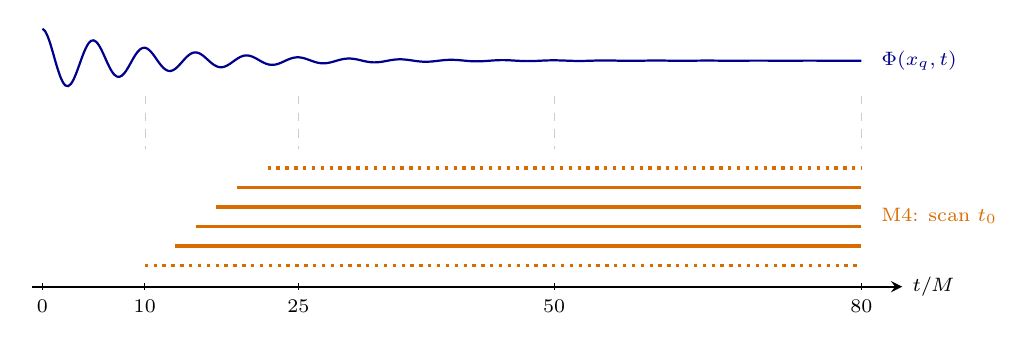
\begin{tikzpicture}[>=stealth, x=0.13cm, y=0.45cm,
                    every node/.style={font=\scriptsize}]
  % --- representative ringdown waveform (top band) ---
  \begin{scope}[yshift=2.6cm]
    \draw[domain=0:80, samples=320, smooth, thick, blue!55!black]
      plot (\x, {0.9*exp(-0.09*\x)*cos(72*\x)});
    \node[blue!55!black, anchor=west] at (81,0)
         {$\Phi(\xq,t)$};
    % light dashed connector to indicate same time axis
    \foreach \x in {10,25,50,80}
      \draw[gray!40, dashed, very thin] (\x,-1.0) -- (\x,-2.5);
  \end{scope}

  % --- M4 windows: vary t_0 in [10,25], fixed t_end = 80 ---
  % plateau block (t_0 = 13..20) drawn solid
  \foreach \t/\y in {13/0.55, 15/1.10, 17/1.65, 19/2.20}
    \draw[orange!85!black, very thick] (\t,\y) -- (80,\y);
  % windows outside the plateau drawn dotted
  \foreach \t/\y in {10/0, 22/2.75}
    \draw[orange!85!black, very thick, dotted] (\t,\y) -- (80,\y);
  \node[orange!85!black, anchor=west] at (81,1.4)
       {M4: scan $t_0$};

  % time axis
  \draw[->, thick] (-1,-0.6) -- (84,-0.6) node[right]{$t/M$};
  \foreach \x in {0,10,25,50,80}
    \draw (\x,-0.5) -- (\x,-0.7) node[below]{$\x$};
\end{tikzpicture}
\caption{M4 schematic: 1-D scan of the start time $t_0$ (six
representative windows of the sixteen-window, step-$1\,M$ scan
shown) with the end time fixed at the usable-signal cutoff
$t=80\,M$. Solid bars belong to the contiguous plateau block and
dotted bars sit outside it. The curve at the top shows a
representative damped waveform on the same time axis.}
\label{fig:m4}
\end{subfigure}

\vspace{1.0em}

%-------------------------------------------------------------
% (b) M5 2-D plateau in (t_0, t_end) plane
%-------------------------------------------------------------
\begin{subfigure}[t]{\textwidth}
\centering
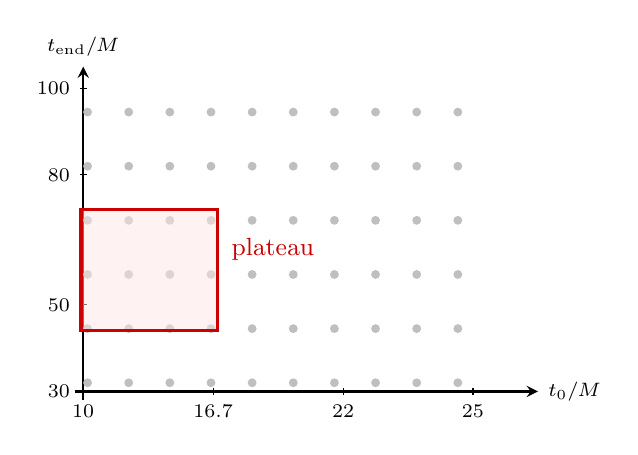
\begin{tikzpicture}[>=stealth, x=0.55cm, y=0.55cm,
                    every node/.style={font=\scriptsize}]
  % axes
  \draw[->, thick] (-0.2,0) -- (10.5,0) node[right]{$t_0/M$};
  \draw[->, thick] (0,-0.2) -- (0,7.5) node[above]{$\tend/M$};
  \foreach \x/\lab in {0/10, 3/16.7, 6/22, 9/25}
    \draw (\x,0.08) -- (\x,-0.08) node[below]{$\lab$};
  \foreach \y/\lab in {0/30, 2/50, 5/80, 7/100}
    \draw (0.08,\y) -- (-0.08,\y) node[left]{$\lab$};

  % grid of (t_0,t_end) candidate windows (10x6 dots)
  \foreach \i in {0,...,9}
    \foreach \j in {0,...,5}
      \fill[gray!50] ({\i*0.95+0.1},{\j*1.25+0.2}) circle (1.6pt);

  % plateau rectangle: t_0 in [10,16.7], t_end in [44,72]
  \draw[red!80!black, very thick, fill=red!10, fill opacity=0.5]
        (-0.05,1.4) rectangle (3.1,4.2);
  \node[red!80!black, anchor=south west, font=\small] at (3.2,2.8)
       {plateau};
\end{tikzpicture}
\caption{M5 schematic: 2-D scan in the $(t_0,\tend)$ plane. Grey
dots are candidate fit windows on a $10\times 6$ grid with
$t_0\in[10,25]\,M$, $\tend\in[30,100]\,M$. The shaded red rectangle
(plateau) is the contiguous $5\times 3$ block of lowest combined
relative scatter measured on the Schwarzschild hFNO waveform,
$t_0\in[10,16.7]\,M$ and $\tend\in[44,72]\,M$.}
\label{fig:m5}
\end{subfigure}
\caption{Fit-window scan schematics for the two plateau-based QNM
extraction methods. (a) M4 sweeps the start time only; (b) M5
sweeps both edges, with the plateau identified as a contiguous
rectangle in the $(t_0,\tend)$ plane.}
\label{fig:windows}
\end{figure}

\FloatBarrier

% --------------------------------------------------------------
\subsubsection{Kerr target-mode protocol}
\label{sec:kerr-qnm}

Kerr extraction introduces a mode-identification problem in addition
to fit-window sensitivity. The labelled $(4,2,0)$ pole can become
subdominant to more slowly decaying late-time components, so a valid
fit need not correspond to the mode being evaluated. We therefore
separate candidate generation from mode identification. Within the
extraction procedure, the Leaver pole identifies the labelled mode but
does not replace any fitted value.

\paragraph{Complex estimators.} For the estimator formulas, let $u$
denote hyperboloidal time and $\tau_{\mathrm d}$ the damping time. A
single complex mode has
$\Psi(\scri,u)=A\exp[(-1/\tau_{\mathrm d}-i\omega_R)(u-u_0)]$,
so $\log|\Psi|$ and the unwrapped phase are linear in $u$. The
c$\Phi$ estimator fits these two slopes. cES instead applies the
ESPRIT construction directly to the complex waveform, without a
Hilbert transform.

\begin{algorithm}[H]
\caption{c$\Phi$ complex-phase estimator.}
\label{alg:cphi}
\begin{algorithmic}[1]
\STATE \textbf{Input:} $\Psi(\scri,u_j)$ on a window $W$.
\STATE $(\widehat a,\widehat b)\gets
  \arg\min_{a,b}\sum_{j\in W}[\log|\Psi_j|-(a+b u_j)]^2$.
\STATE $(\widehat c,\widehat d)\gets
  \arg\min_{c,d}\sum_{j\in W}
  [\operatorname{unwrap}\arg\Psi_j-(c+d u_j)]^2$.
\STATE \textbf{return}
  $(\widehat\omega_R,\widehat\tau_{\mathrm d})
  =(-\widehat d,-1/\widehat b)$.
\end{algorithmic}
\end{algorithm}

\begin{algorithm}[H]
\caption{cES complex ESPRIT estimator.}
\label{alg:ces}
\begin{algorithmic}[1]
\STATE \textbf{Input:} $\Psi(\scri,u_j)$ on a window $W$ and
       model order $K$.
\STATE $\{z_n,c_n\}_{n=0}^{K-1}\gets\operatorname{ESPRIT}_K(\Psi_W)$
       using Eq.~\eqref{eq:esprit-poles}.
\STATE $(\widehat\omega_{R,n},\widehat\tau_{\mathrm d,n})\gets
  [-\operatorname{Im}\log z_n/\Delta u,
  -\Delta u/\operatorname{Re}\log z_n]$.
\STATE \textbf{return} the physical pole selected below.
\end{algorithmic}
\end{algorithm}

\paragraph{Candidate generation and mode identification.} The Leaver
damping time $\tau_{\mathrm{ref}}$ sets all window scales. Targeted M3
($K=6$) and M4 fits are applied separately to
$\operatorname{Re}\Psi$ and $\operatorname{Im}\Psi$ on a
$3\times3$ grid with
$u_{\mathrm{start}}/\tau_{\mathrm{ref}}\in[2,5]$,
$u_{\mathrm{end}}/\tau_{\mathrm{ref}}\in[7,12]$ and duration at
least $3\tau_{\mathrm{ref}}$; cES scans the same windows with
$K\in\{3,4,5,6\}$. M2 on both field components and c$\Phi$ provide
late-time cross-checks on an $8\times6$ grid with
$u_{\mathrm{start}}/\tau_{\mathrm{ref}}\in[4,9]$ and
$u_{\mathrm{end}}/\tau_{\mathrm{ref}}\in[10,14]$, with an
envelope-slope upper cutoff. Multi-mode fits retain the pole nearest
the labelled Leaver pole, and each scan is reduced to its median
candidate. Candidates more than $12\%$ from
$\omega_{R,\mathrm{ref}}$ are rejected. Complete per-estimator
results are reported in Appendix~\ref{app:kerr-extractors}.
% --------------------------------------------------------------
\subsection{Reporting convention}
\label{sec:reporting}

Ringdown parameter recovery is sensitive to the waveform model, fit
interval and extraction procedure, and frequency and damping time can
exhibit markedly different biases, so averaging across the estimator
suite would combine stable fits with identifiable failures
\citep{Berti2007matched,Isi2021priors}. The reported summaries
therefore give the smallest Leaver error attained for each quantity
and record the best accuracy achieved by the suite, not the expected
performance of a fixed estimator.
No Schwarzschild fit uses Leaver values. For the Schwarzschild summary
statistics, the estimator with the smallest Leaver error is selected
separately for frequency and damping time after extraction. The reproduction
comparison is restricted to M1 and M2, while M4 scatter measures
fit-window sensitivity only.
For Kerr, Leaver values identify the $(4,2,0)$ candidate among
multi-mode fits. After extraction, the candidate with the smallest
frequency error and the candidate with the smallest damping-time error
against Leaver are reported separately. Complete per-estimator results
are given in Appendix~\ref{app:kerr-extractors}, and each reported
quantity identifies the selected estimator.

% =====================================================================
% =============================================================
% Section 4: Results
% =============================================================
\section{Results}\label{sec:results}

The three models are presented in a uniform format: field
accuracy against the FD reference (snapshots, pointwise error,
and summary metrics), the ringdown waveform at the observer,
and the QNM extraction table of the five methods of
Sec.~\ref{sec:qnm-methods} under the reporting convention of
Sec.~\ref{sec:reporting}. Sections~\ref{sec:res-repro}%
--\ref{sec:res-fwd} treat one black hole at a time
(reproduction, enhanced forward);
Sec.~\ref{sec:res-hyb} evaluates the hybrid
surrogate on the canonical BH and on a $100$-BH test
population; and Sec.~\ref{sec:res-kerr} generalises the hybrid
to a population of rotating (Kerr) black holes. Supporting
scans and diagnostics are
collected in Appendix~\ref{app:supp}.
Table~\ref{tab:results-summary} summarises the principal
quantitative results of the three Schwarzschild models; the
Kerr generalisation is summarised separately in
Table~\ref{tab:kerr-summary}.

\begin{table}[!htbp]
\centering
\caption{Summary of the principal quantitative results.
Field errors are computed against the FD reference over the
full $(x,t)$ grid: RMSD in field units
($|\Phi|_{\max} \approx 1$) and relative $L^{2}$ norm (RL2).
QNM errors are relative errors against the Leaver
continued-fraction values $M\omega_{0} = 0.3737$,
$\tau_{0}/M = 11.241$, under the reporting convention of
Sec.~\ref{sec:reporting}: each entry is the smallest error over
the M1--M5 estimator suite of Sec.~\ref{sec:qnm-methods} --- the
Leaver-closest of five extractors, none of which sees the
reference during extraction --- labelled with the estimator
used; the per-estimator breakdown is in
Tables~\ref{tab:repro-qnm}, \ref{tab:fwd-qnm}
and~\ref{tab:hyb-canonical}. All QNM errors are read at the common
observer $\xq = 10\,M$ (window $[10,50]\,M$ for the PINN rows,
$[10,100]\,M$ for the hybrid).
Population-row QNM
errors are medians over the $100$-BH test set; the hybrid
population field entries are population means. For the reproduction rows
the corresponding values in \citet[Table~2]{Patel2024pinn} are
$\mathrm{RL2} = 28.06\%$ (Zerilli) and $23.59\%$
(Regge--Wheeler); for the hybrid rows the coarse-up baseline
gives $\mathrm{RL2} = 4.93\%$ (canonical) and $6.11\%$
(population). Dashes denote quantities not applicable to,
or not evaluated for, that row.}
\label{tab:results-summary}
\footnotesize
\setlength{\tabcolsep}{4pt}
\renewcommand{\arraystretch}{1.15}
\begin{tabular}{@{}lllcccc@{}}
\toprule
Sec. & Model & Evaluation & Field RMSD & RL2 [\%]
     & $|\Delta\omega|/\omega$ [\%] & $|\Delta\tau|/\tau$ [\%] \\
\midrule
\ref{sec:res-repro} & Reproduction (Zerilli)       & canonical BH             & $1.83\times 10^{-3}$ & $1.30$  & $1.08$~(M1)  & $1.50$~(M2)  \\
\ref{sec:res-repro} & Reproduction (Regge--Wheeler) & canonical BH            & $3.77\times 10^{-3}$ & $2.67$  & $0.56$~(M1)  & $1.56$~(M2)  \\
\ref{sec:res-fwd}   & Enhanced forward PINN        & canonical BH             & $8.17\times 10^{-4}$ & $0.58$  & $0.029$~(M4) & $1.99$~(M2)  \\
\ref{sec:res-hyb}   & Hybrid surrogate             & canonical BH             & $6.28\times 10^{-4}$ & $0.445$ & $0.047$~(M5) & $1.34$~(M1)  \\
\ref{sec:res-hyb}   & Hybrid surrogate             & $100$-BH population      & $9.68\times 10^{-4}$ & $0.648$ & $0.152$~(M4) & $0.528$~(M4) \\
\bottomrule
\end{tabular}
\end{table}

% --------------------------------------------------------------
\subsection{Faithful reproduction of the prior-work baseline}
\label{sec:res-repro}

We first establish that the pipeline reproduces the prior-work
baseline of \citet{Patel2024pinn} --- the only previous
time-domain PINN treatment of these $\ell = 2$ master
equations --- before any methodological change is introduced;
it does, improving on the published field errors by an order
of magnitude. The forward PINN is trained at their exact
settings (Table~\ref{tab:fwd-hyper}: uniform collocation
resampling, their loss weights and optimiser budget), i.e.\
without the enhancements of Sec.~\ref{sec:res-fwd}, on both
the even-parity (Zerilli) and odd-parity (Regge--Wheeler)
potentials.

\paragraph{Field accuracy.} At matched settings the
reproduction reaches $\mathrm{RL2} = 1.30\%$
(RMSD $1.83\times 10^{-3}$) on the Zerilli potential and
$\mathrm{RL2} = 2.67\%$ (RMSD $3.77\times 10^{-3}$, MAD
$2.53\times 10^{-3}$) on the Regge--Wheeler potential, against
$28.06\%$ and $23.59\%$ respectively in
\citet[Table~2]{Patel2024pinn} --- a factor of $\sim\!21$
(Zerilli) and $\sim\!9$ (Regge--Wheeler) at identical
architecture, loss weights and optimiser budget; the remaining
differences are implementation-level (double-precision
training and the outgoing-pulse initial velocity of
Sec.~\ref{sec:fwd-pinn}).
Snapshot overlays and global error maps are shown in
Figs.~\ref{fig:repro-zer-field} and~\ref{fig:repro-rw-field},
and the training histories in Fig.~\ref{fig:repro-loss}.

\begin{figure}[!htbp]
\centering
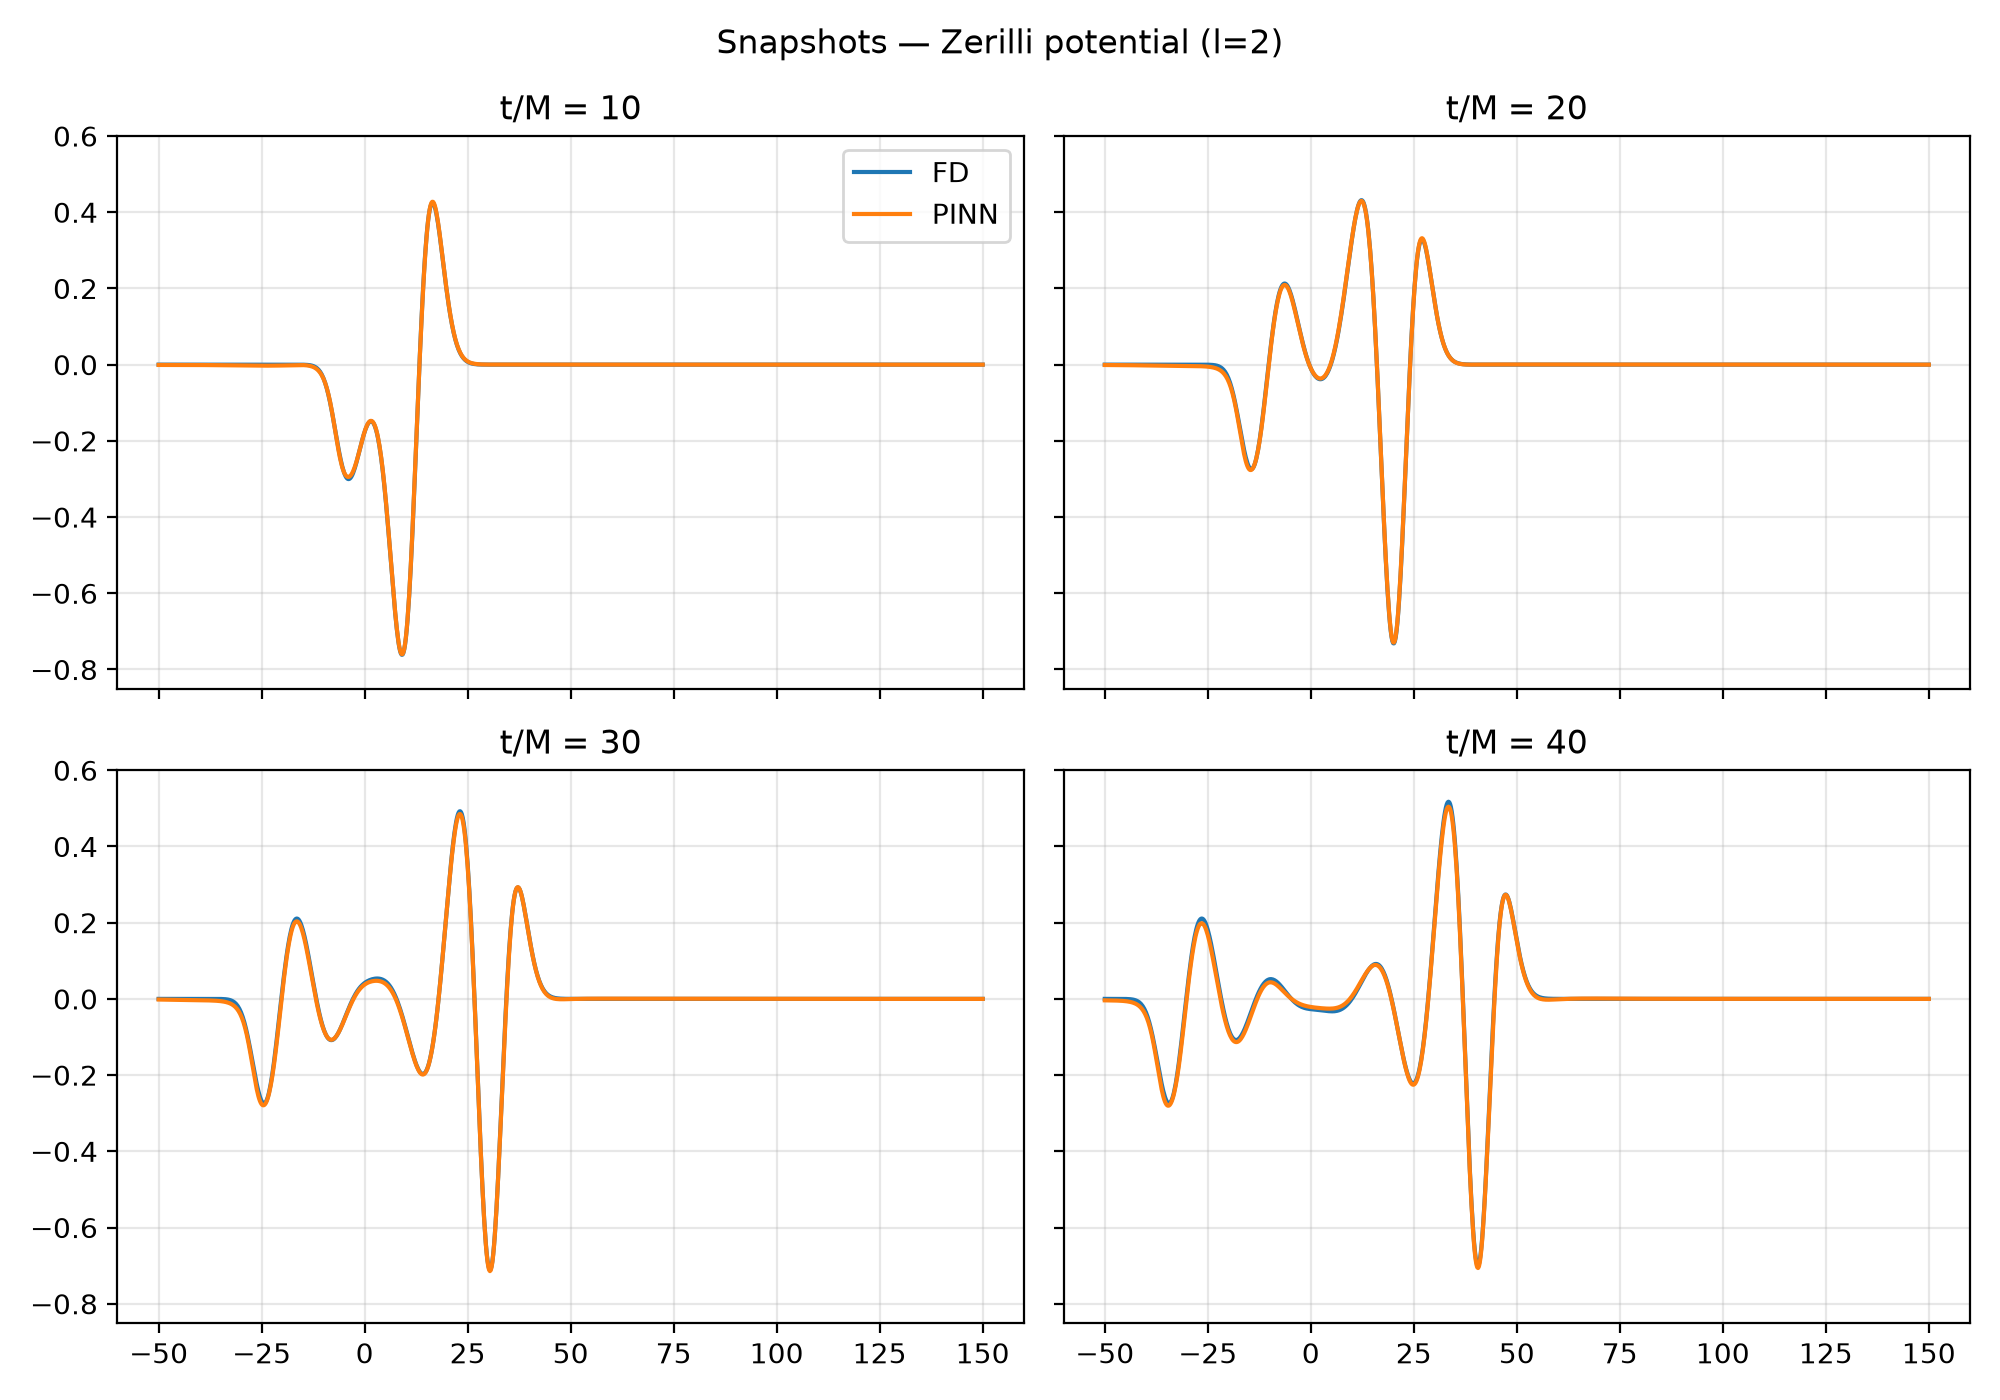
\includegraphics[width=0.82\textwidth]{../outputs/pinn/zerilli_l2_paper/snapshots.png}\\[0.4em]
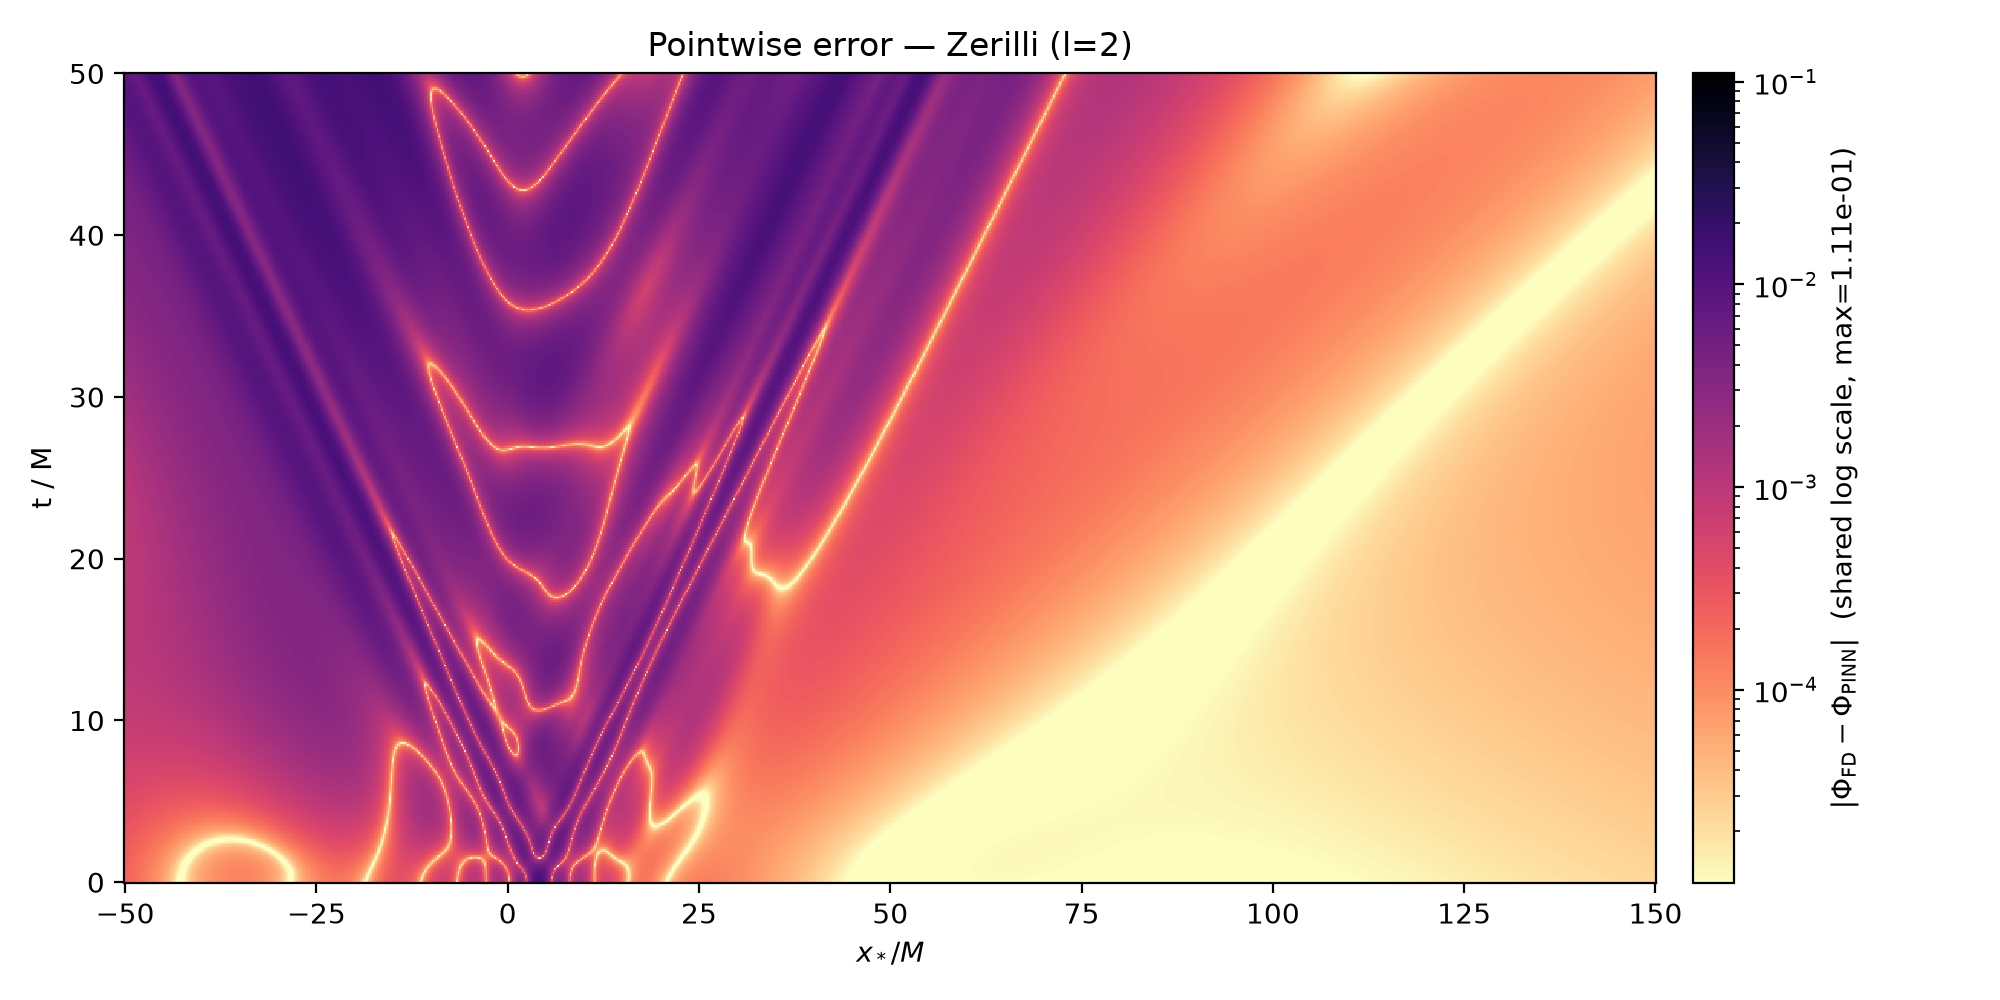
\includegraphics[width=0.88\textwidth]{../outputs/pinn/zerilli_l2_paper/error_heatmap.png}
\caption{Faithful reproduction on the Zerilli potential. Top:
snapshots of $\Phi(x,t)$ at $t/M \in \{10,20,30,40\}$ overlaid
for the reproduced PINN and the FD reference; the curves are
visually indistinguishable on this scale. Bottom: global
pointwise error $|\Phi_{\mathrm{FD}} - \Phi_{\mathrm{PINN}}|$
on $x \in [-50,150]\,M$, $t \in [0,50]\,M$, peaking at
$\sim\!1.0\times 10^{-2}$ on the outgoing wavefront,
consistent with the gridwise RMSD of $1.83\times 10^{-3}$.}
\label{fig:repro-zer-field}
\end{figure}

\begin{figure}[!htbp]
\centering
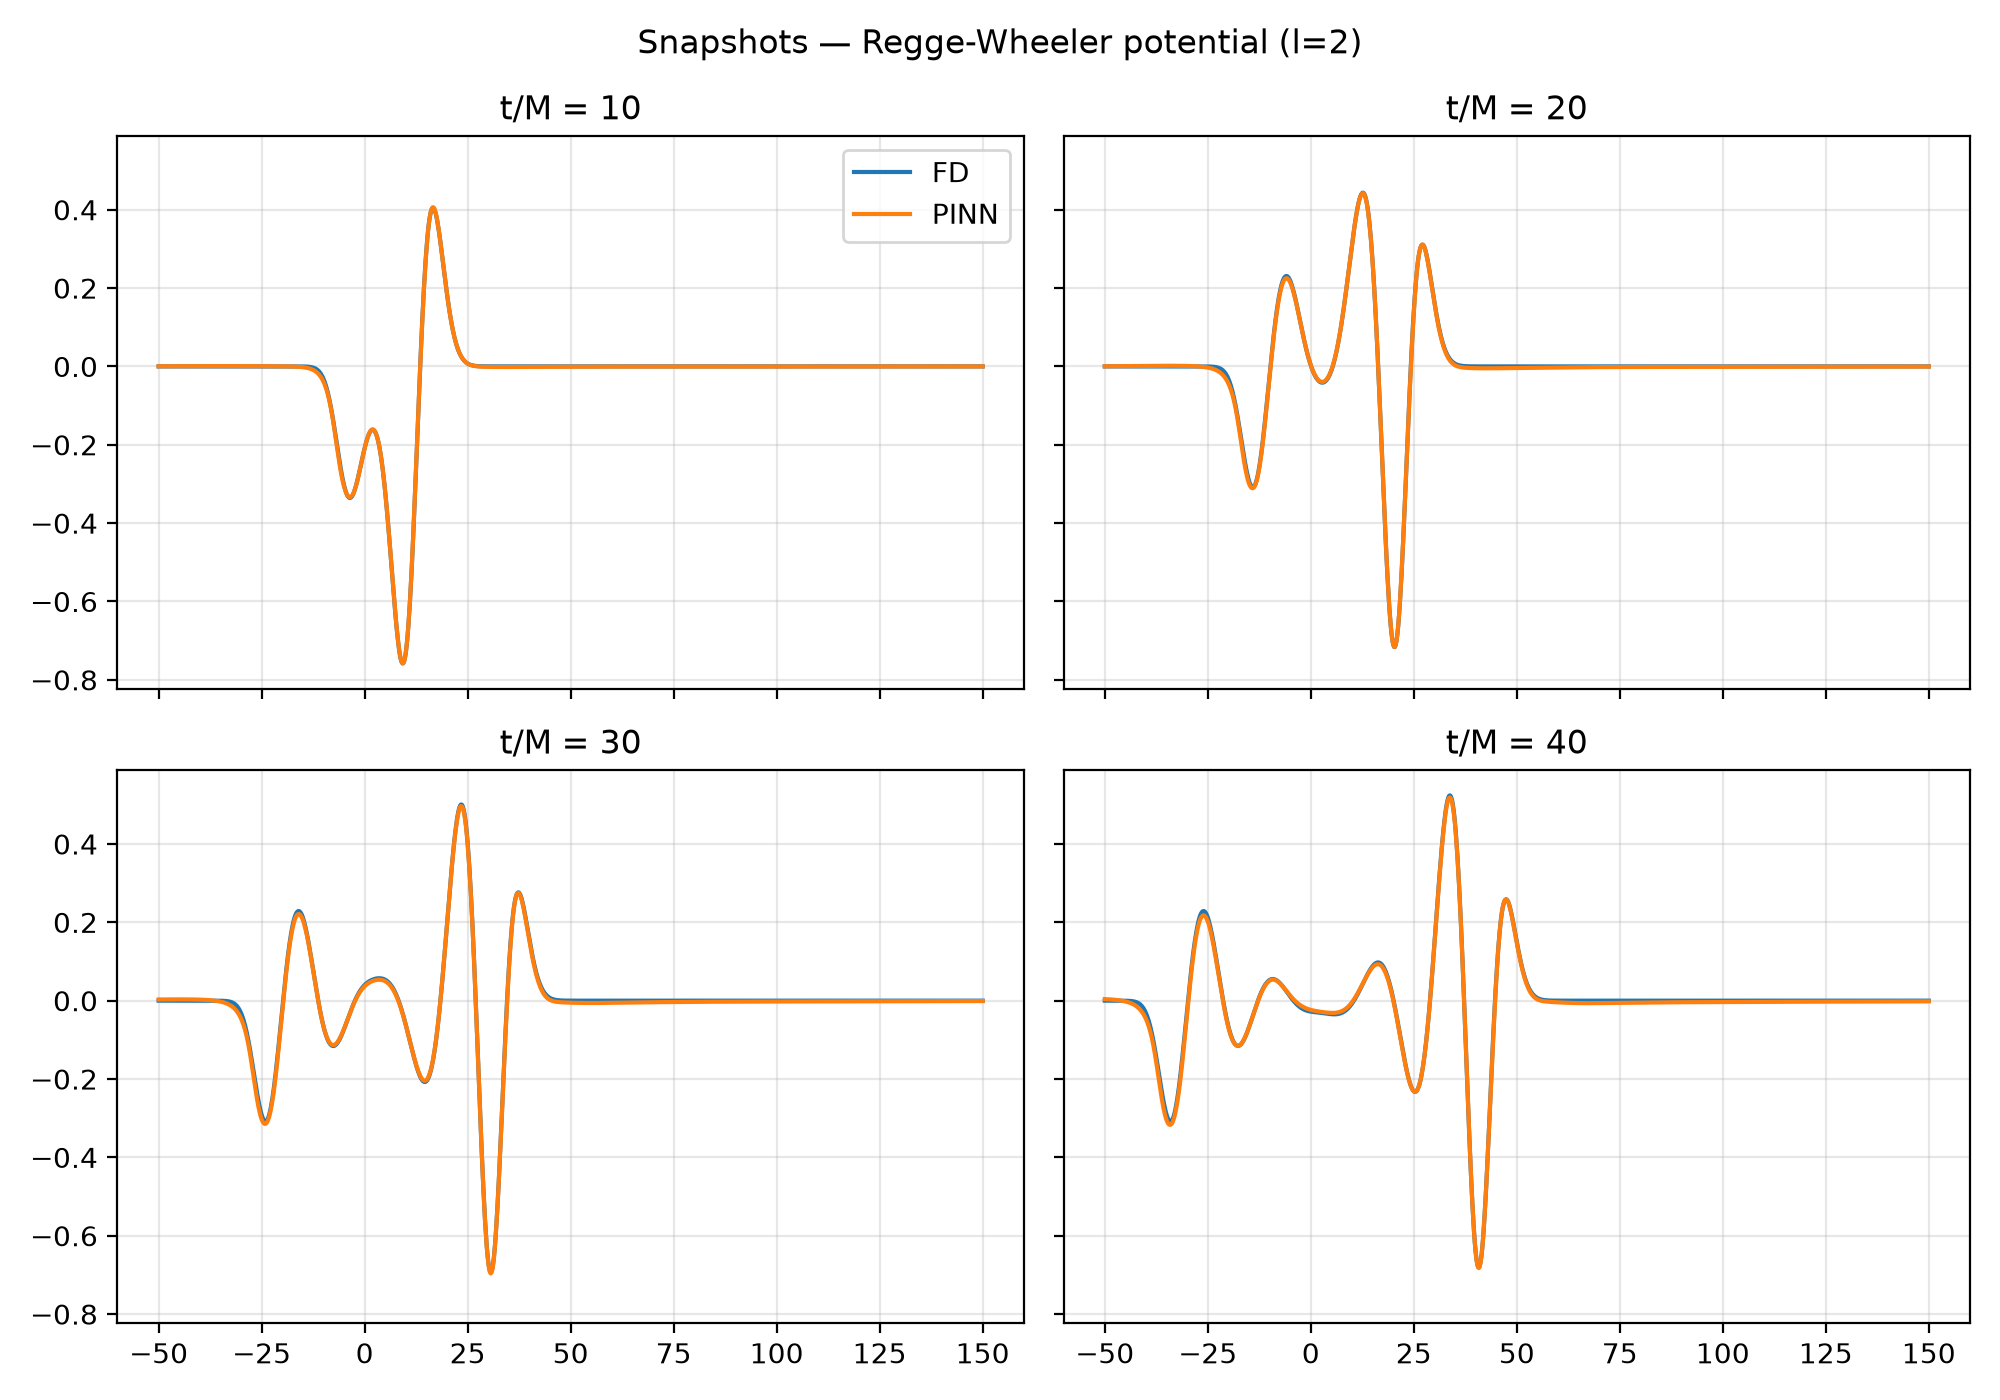
\includegraphics[width=0.82\textwidth]{../outputs/pinn/regge_wheeler_l2_paper/snapshots.png}\\[0.4em]
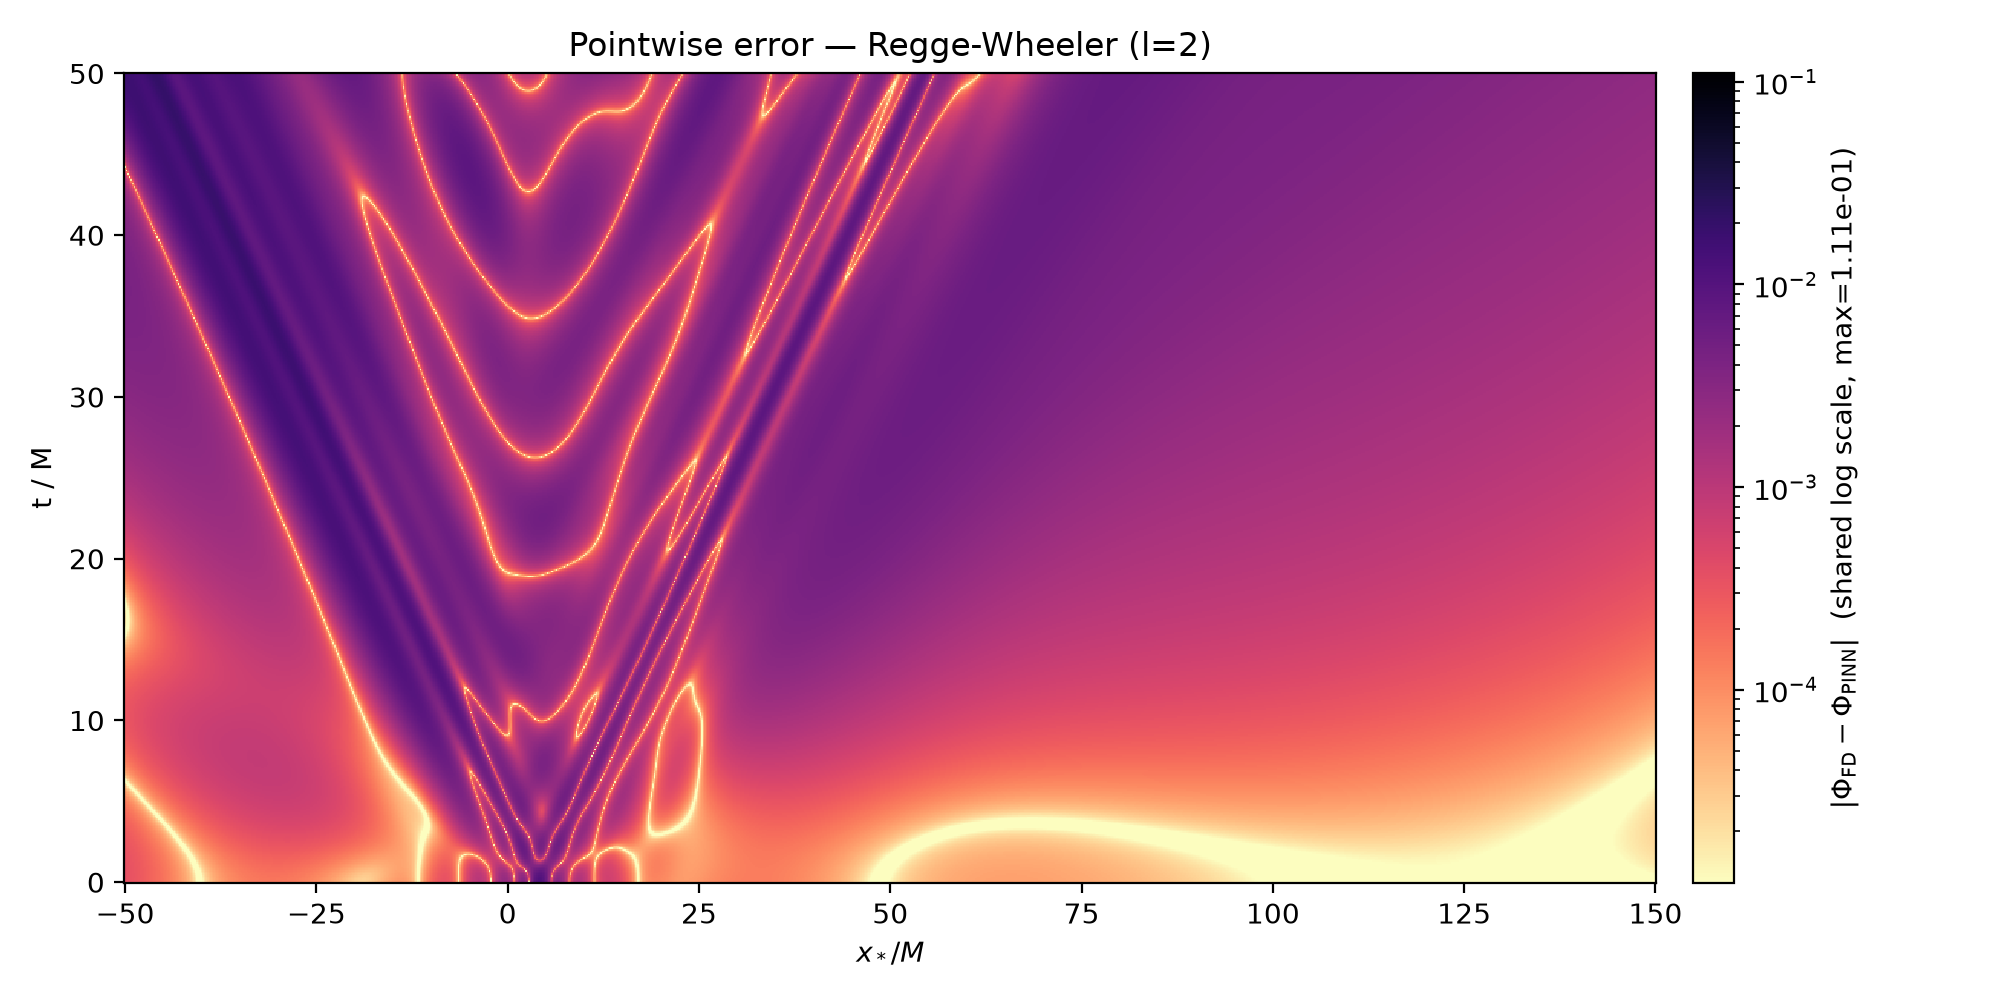
\includegraphics[width=0.88\textwidth]{../outputs/pinn/regge_wheeler_l2_paper/error_heatmap.png}
\caption{Faithful reproduction on the Regge--Wheeler potential.
Top: snapshots of $\Phi(x,t)$ at $t/M \in \{10,20,30,40\}$
overlaid for the reproduced PINN and the FD reference. Bottom:
global pointwise error $|\Phi_{\mathrm{FD}} - \Phi_{\mathrm{PINN}}|$
on the same domain, concentrated on the left-going late-time
characteristic, consistent with the gridwise RMSD of
$3.77\times 10^{-3}$.}
\label{fig:repro-rw-field}
\end{figure}

\paragraph{QNM extraction.} Table~\ref{tab:repro-qnm} applies
the two extraction methods used by \citet{Patel2024pinn} (M1
and M2, their ``PINN1''/``PINN2'') to the reproduced fields at
$\xq = 10\,M$. The frequencies agree at the one-to-two-percent
level on both potentials; the damping time, the observable most
sensitive to field quality, improves several-fold: from
$14.42\%$ to $1.50\%$ (Zerilli) and from $5.39\%$ to $1.56\%$
(Regge--Wheeler, M2). The ringdown at the observer, with the
damped-cosine reconstructions overlaid, is shown in
Figs.~\ref{fig:repro-zer-ringdown}
and~\ref{fig:repro-rw-ringdown}.

\begin{table}[!htbp]
\centering
\caption{Faithful reproduction: QNM extraction at $\xq = 10\,M$
with the two methods of \citet{Patel2024pinn} (M1 = FFT $+$
log-envelope, M2 = damped-cosine NLS; their PINN1/PINN2),
applied to the reproduced PINN fields on both potentials.
Reference values are the Leaver continued-fraction Schwarzschild
$\ell = 2$ fundamental $M\omega_0 = 0.3737$,
$\tau_0/M = 11.241$; \citet{Patel2024pinn} quote their
percentage errors against the rounded reference
$M\omega_0 = 0.374$. Bold entries mark the damping-time
improvement discussed in the text.}
\label{tab:repro-qnm}
\footnotesize
\setlength{\tabcolsep}{4pt}
\renewcommand{\arraystretch}{1.1}
\begin{tabular}{@{}llcccc@{}}
\toprule
 & & \multicolumn{2}{c}{This work} & \multicolumn{2}{c}{\citet{Patel2024pinn}} \\
\cmidrule(lr){3-4}\cmidrule(l){5-6}
Potential & Method & $M\omega$ (err) & $\tau/M$ (err) & $M\omega$ (err) & $\tau/M$ (err) \\
\midrule
Zerilli & M1 & $0.3697$ ($1.08\%$) & $10.671$ ($5.07\%$) & $0.375$ ($0.29\%$) & $10.089$ ($10.25\%$) \\
Zerilli & M2 & $0.3784$ ($1.25\%$) & $11.410$ ($\mathbf{1.50\%}$) & $0.376$ ($0.52\%$) & $9.620$ ($14.42\%$) \\
Regge--Wheeler & M1 & $0.3716$ ($0.56\%$) & $10.753$ ($4.34\%$) & $0.373$ ($0.11\%$) & $10.474$ ($6.82\%$) \\
Regge--Wheeler & M2 & $0.3811$ ($1.97\%$) & $11.416$ ($\mathbf{1.56\%}$) & $0.383$ ($2.51\%$) & $10.636$ ($5.39\%$) \\
\bottomrule
\end{tabular}
\end{table}

\begin{figure}[!htbp]
\centering
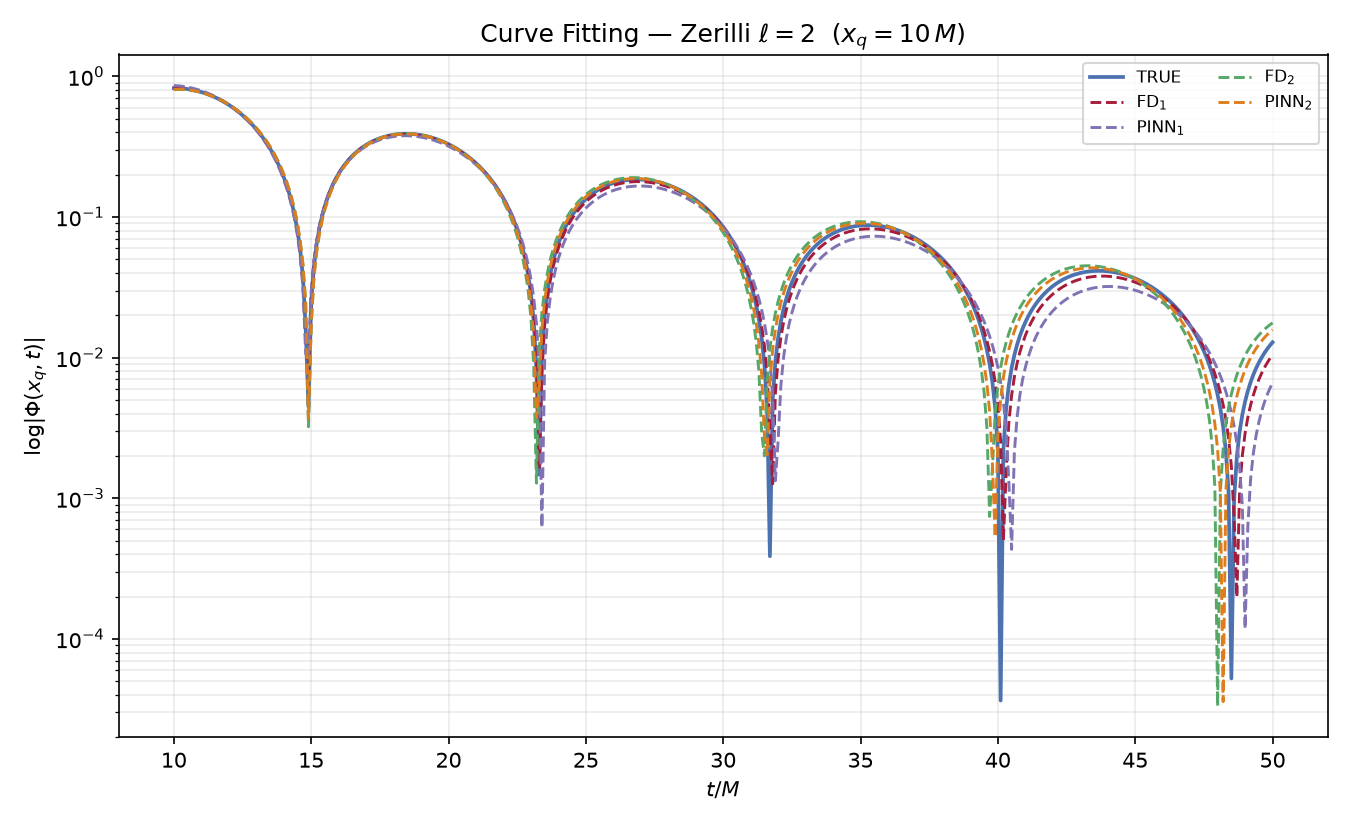
\includegraphics[width=0.80\textwidth]{../outputs/pinn/zerilli_l2_paper/curve_fitting.png}
\caption{Faithful reproduction on the Zerilli potential:
ringdown at the observer. $\log_{10}|\Phi(\xq{=}10\,M, t)|$ for
the reproduced PINN and FD waveforms with the damped-cosine
reconstructions of the M1 and M2 extractions of
Table~\ref{tab:repro-qnm} overlaid.}
\label{fig:repro-zer-ringdown}
\end{figure}

\begin{figure}[!htbp]
\centering
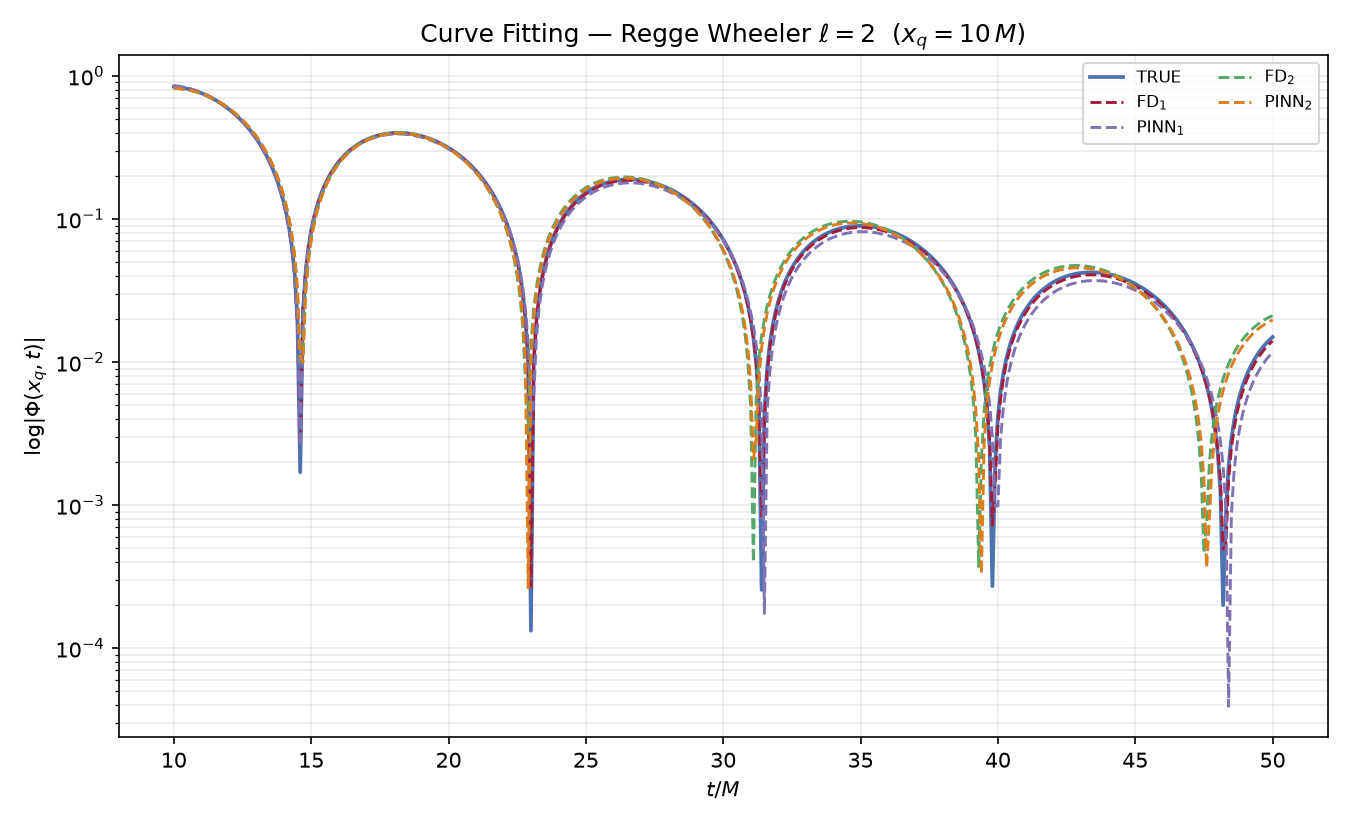
\includegraphics[width=0.80\textwidth]{../outputs/pinn/regge_wheeler_l2_paper/curve_fitting.png}
\caption{Faithful reproduction on the Regge--Wheeler potential:
ringdown at the observer. $\log_{10}|\Phi(\xq{=}10\,M, t)|$ for
the reproduced PINN and FD waveforms with the damped-cosine
reconstructions of the M1 and M2 extractions of
Table~\ref{tab:repro-qnm} overlaid.}
\label{fig:repro-rw-ringdown}
\end{figure}

\begin{figure}[!htbp]
\centering
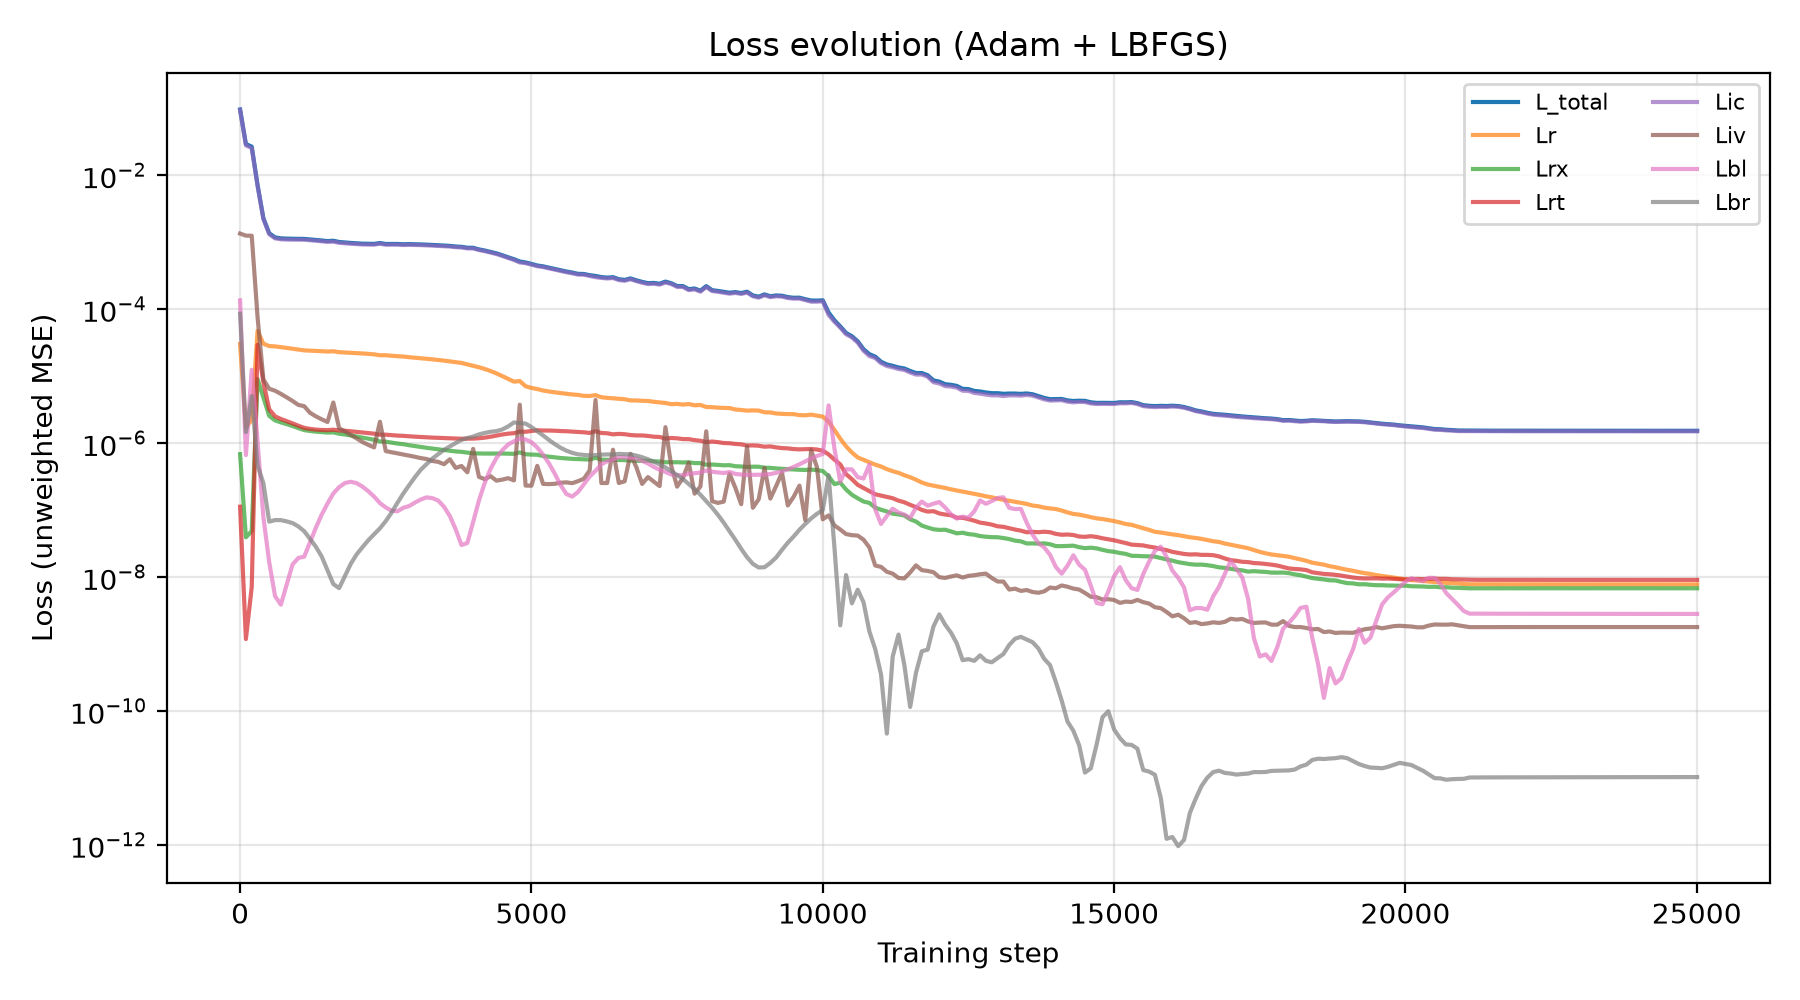
\includegraphics[width=0.80\textwidth]{../outputs/pinn/zerilli_l2_paper/loss.png}\\[0.4em]
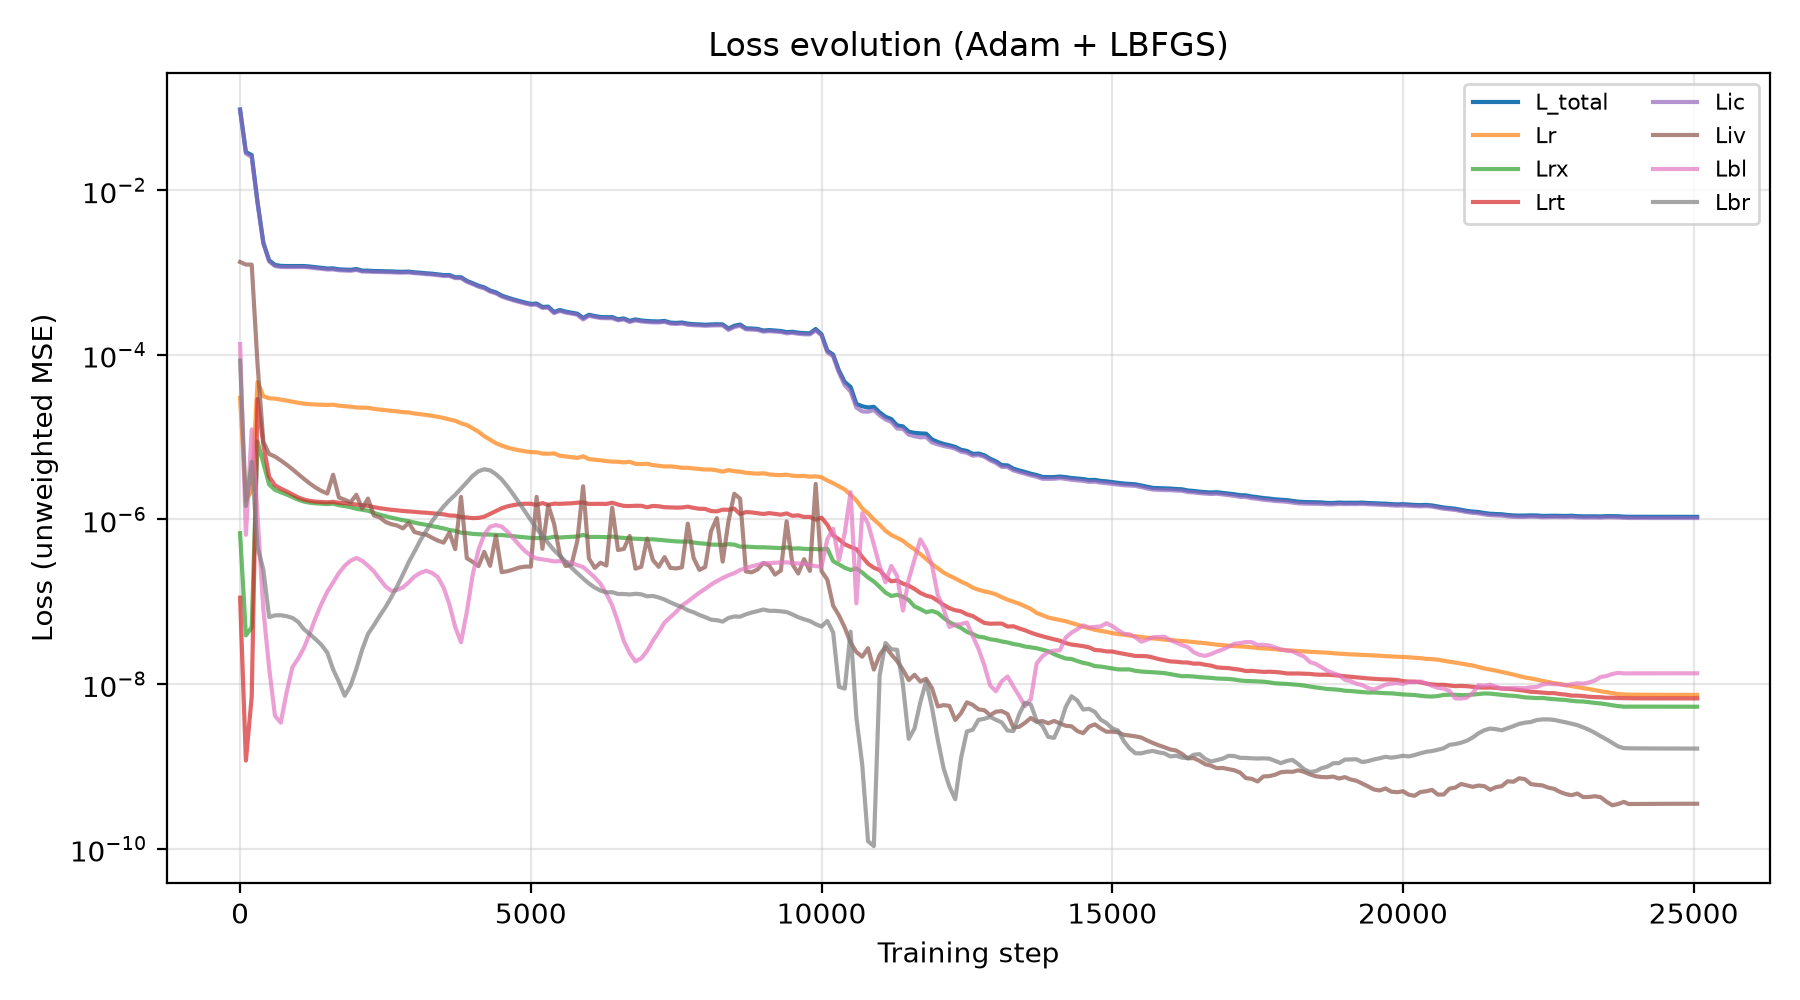
\includegraphics[width=0.80\textwidth]{../outputs/pinn/regge_wheeler_l2_paper/loss.png}
\caption{Faithful-reproduction training histories: total loss
and the seven unweighted components versus training step, with
the Adam--L-BFGS transition at iteration $10{,}000$ marked.
Top: Zerilli. Bottom: Regge--Wheeler.}
\label{fig:repro-loss}
\end{figure}

\paragraph{Isospectral consistency.} The two potentials share
the same QNM spectrum \citep{Chandrasekhar1975}, so a
consistent pipeline must recover compatible $(\omega,\tau)$
from both --- and it does: the M2 damping-time errors agree to
within $0.06$ percentage points ($1.50\%$ versus $1.56\%$),
against a nine-point spread in \citet[Table~3]{Patel2024pinn}.
Having established equivalent behaviour on both potentials,
the remainder of this paper reports on the Zerilli equation.

\FloatBarrier

% --------------------------------------------------------------
\subsection{Enhanced forward PINN}
\label{sec:res-fwd}

How far can the forward field error be driven down at fixed
architecture, and what QNM accuracy does that buy? Starting
from the faithful reproduction of
Sec.~\ref{sec:res-repro}, the enhanced forward PINN doubles the
L-BFGS budget and replaces uniform resampling with the
residual-greedy sampling of Sec.~\ref{sec:fwd-pinn}, all other
settings unchanged. On the FD grid
$x \in [-50,150]\,M$, $t \in [0,50]\,M$ the field-accuracy
metrics are
\begin{equation}
  \mathrm{RMSD} = 8.17\times 10^{-4}, \qquad
  \mathrm{MAD}  = 4.99\times 10^{-4}, \qquad
  \mathrm{RL2}  = 5.79\times 10^{-3},
  \label{eq:fwd-metrics}
\end{equation}
where $\mathrm{RMSD}$ and $\mathrm{MAD}$ are the root-mean-square
and mean-absolute differences $\Phi_\theta - \Phi_{\mathrm{FD}}$ in
absolute units (peak $|\Phi| \approx 0.7$ on the domain), and
$\mathrm{RL2}$ is their relative $L^2$ norm.
This $\mathrm{RL2} = 0.58\%$ is a factor of $\sim\!50$ smaller
than the $\mathrm{RL2} = 28.06\%$ of
\citet[Table~2, Zerilli row]{Patel2024pinn} and a further
factor of $\sim\!2.2$ below the reproduction; the MAD
improvement is $5.0\times 10^{-4}$ versus their
$1.82\times 10^{-2}$, a factor of $\sim\!36$. Field accuracy
at the snapshot times, the global pointwise error, and the
per-component loss history are shown in
Figs.~\ref{fig:fwd-field}--\ref{fig:fwd-loss}.

\begin{figure}[!htbp]
\centering
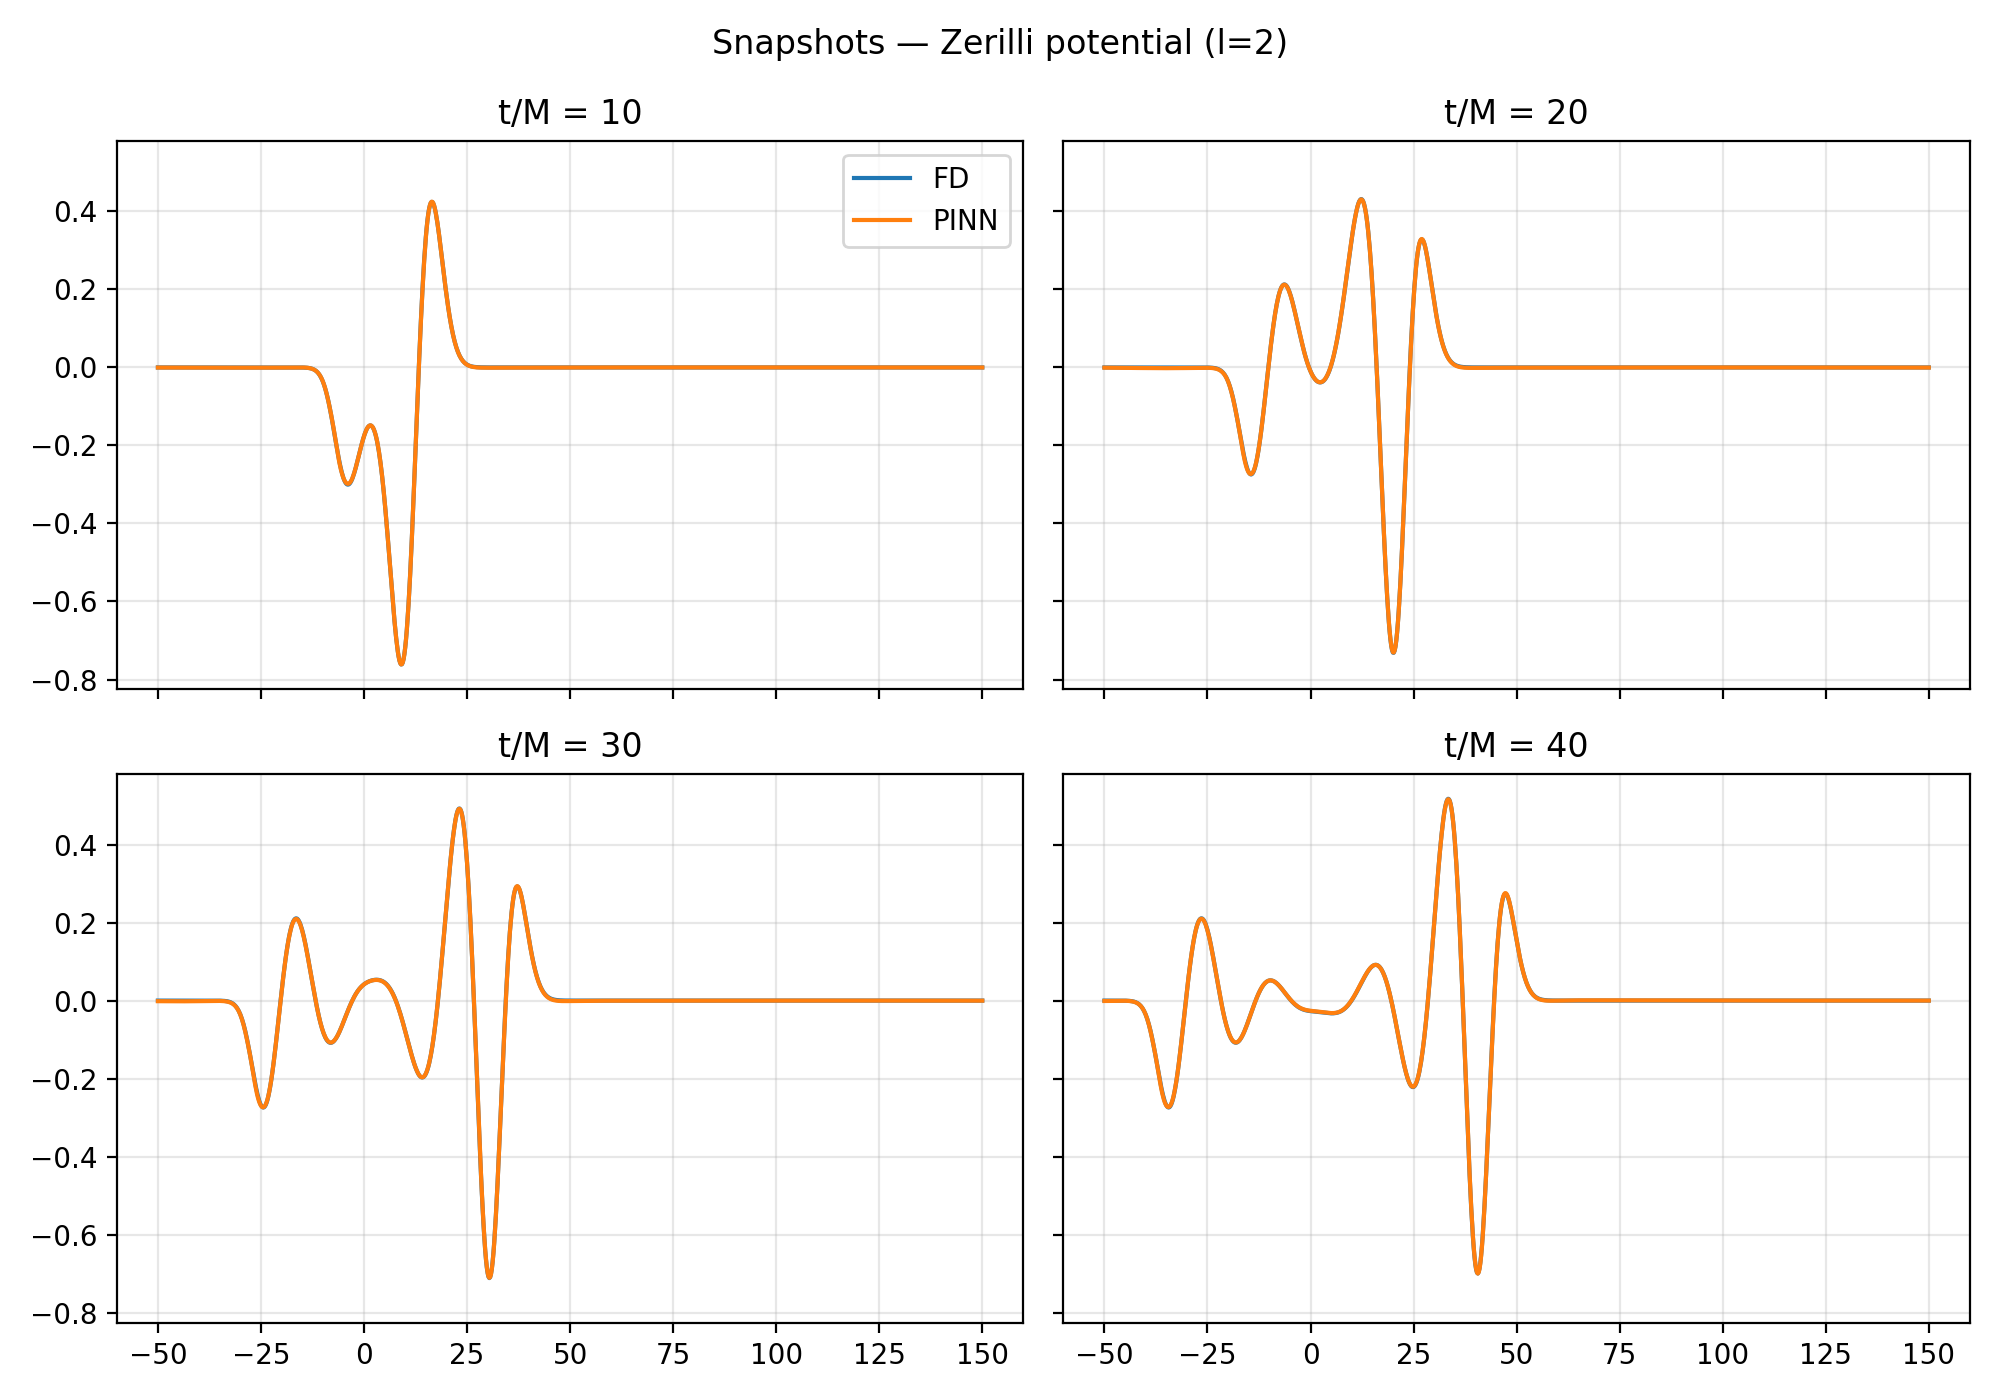
\includegraphics[width=0.82\textwidth]{../outputs/pinn/zerilli_l2_greedy_f03_lbfgs30k/snapshots.png}\\[0.4em]
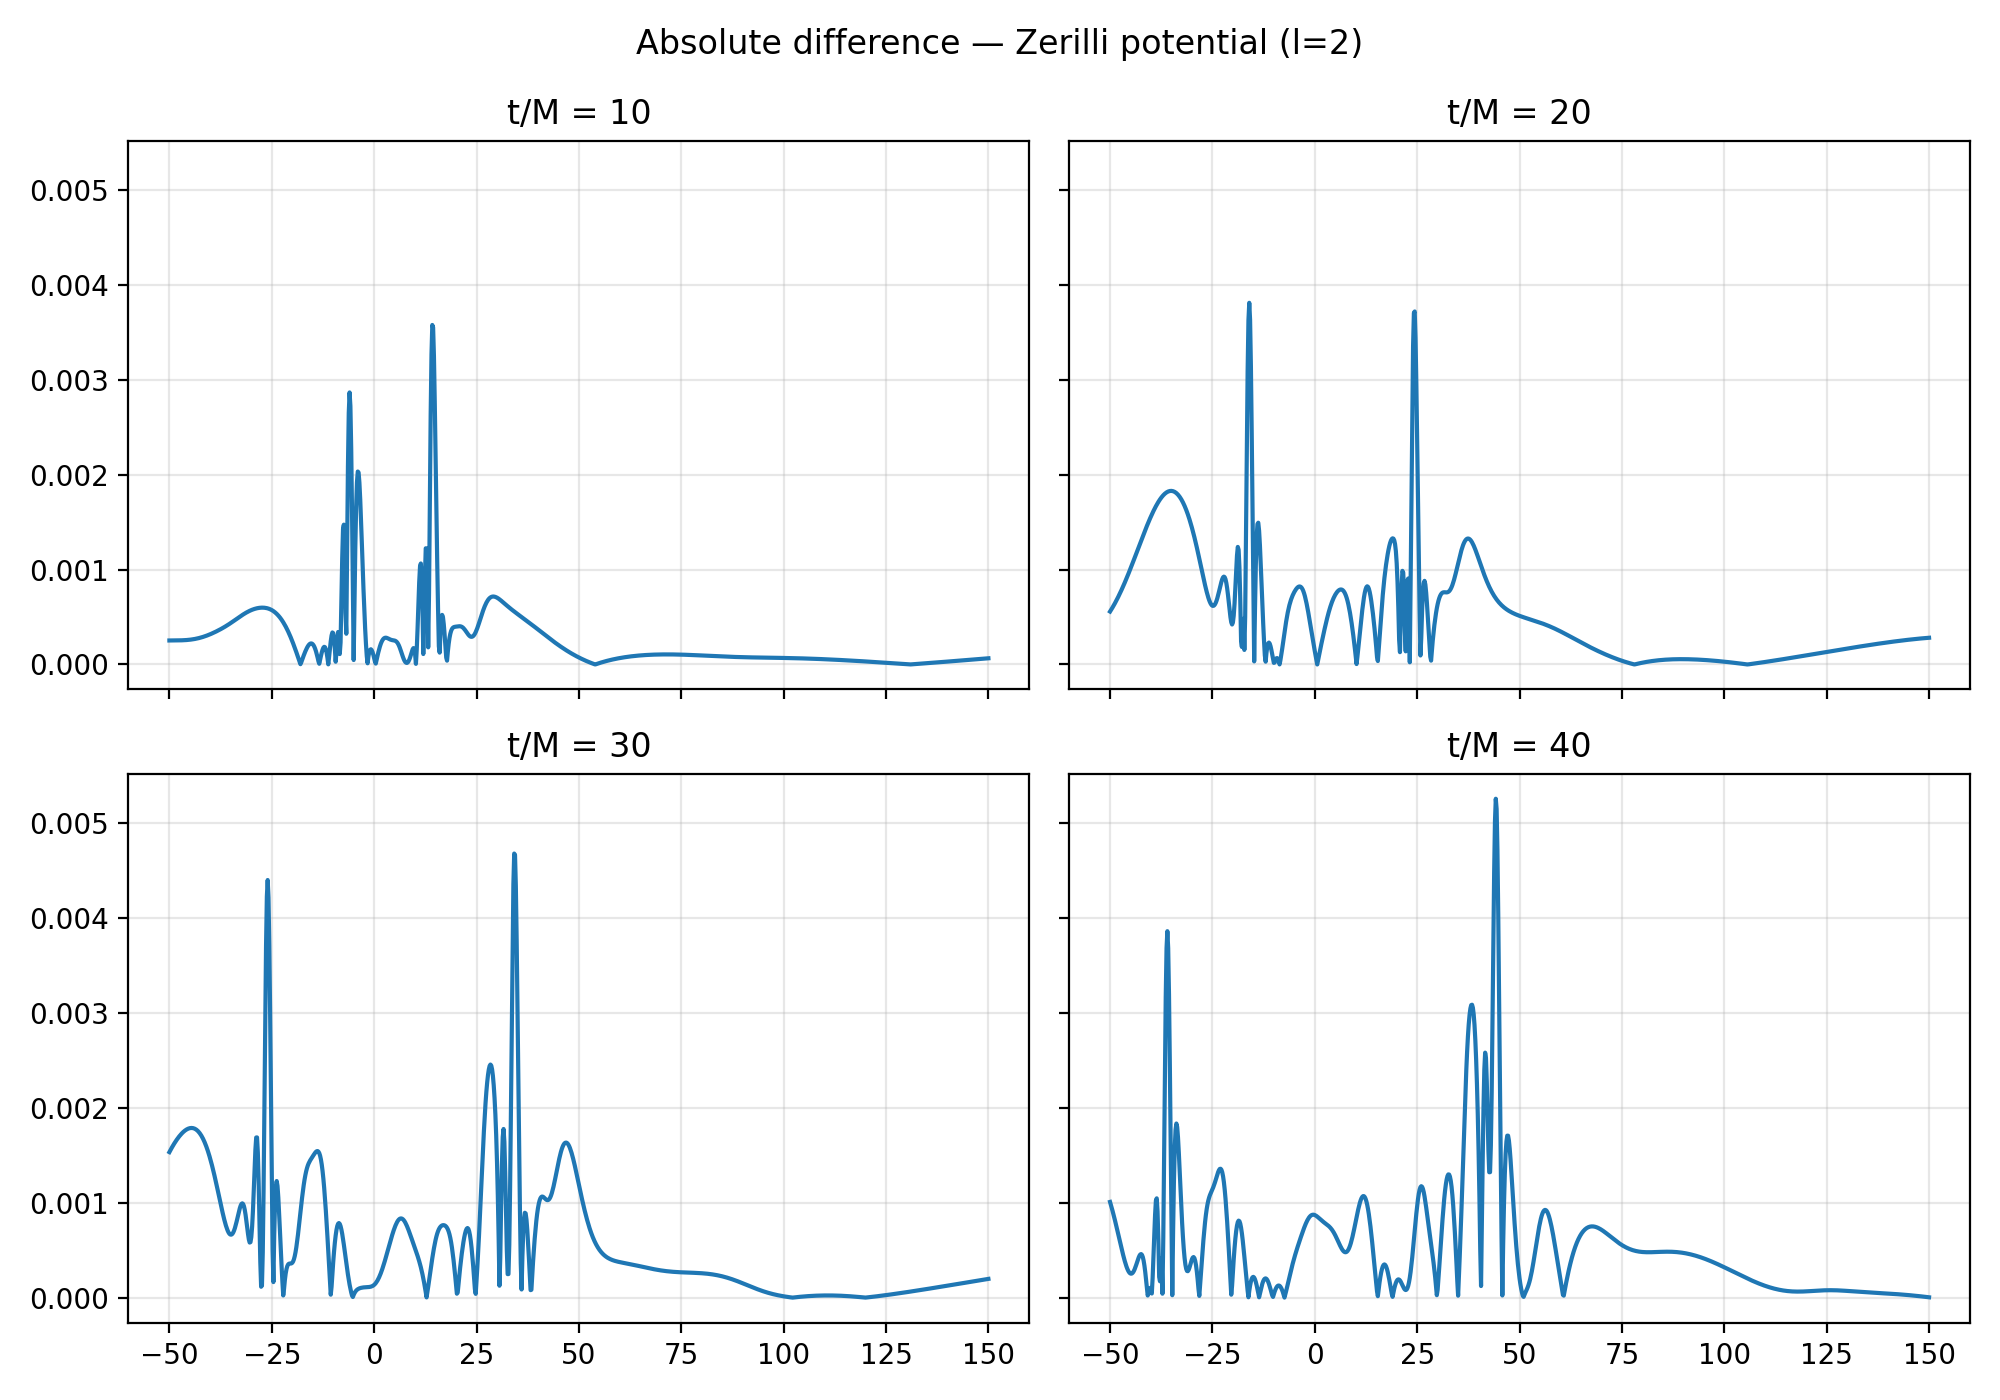
\includegraphics[width=0.82\textwidth]{../outputs/pinn/zerilli_l2_greedy_f03_lbfgs30k/abs_diff_snapshots.png}
\caption{Forward PINN versus FD reference at the snapshot times.
Top: snapshots of $\Phi(x,t)$ at four times
$t/M\in\{10,20,30,40\}$ overlaid for the PINN and the FD
reference; the two curves are visually indistinguishable on this
scale. Bottom: pointwise $|\Phi_\theta - \Phi_{\mathrm{FD}}|$
at the same four times, concentrated near the potential barrier
and remaining below $\sim\!5\times 10^{-3}$ throughout.}
\label{fig:fwd-field}
\end{figure}

\begin{figure}[!htbp]
\centering
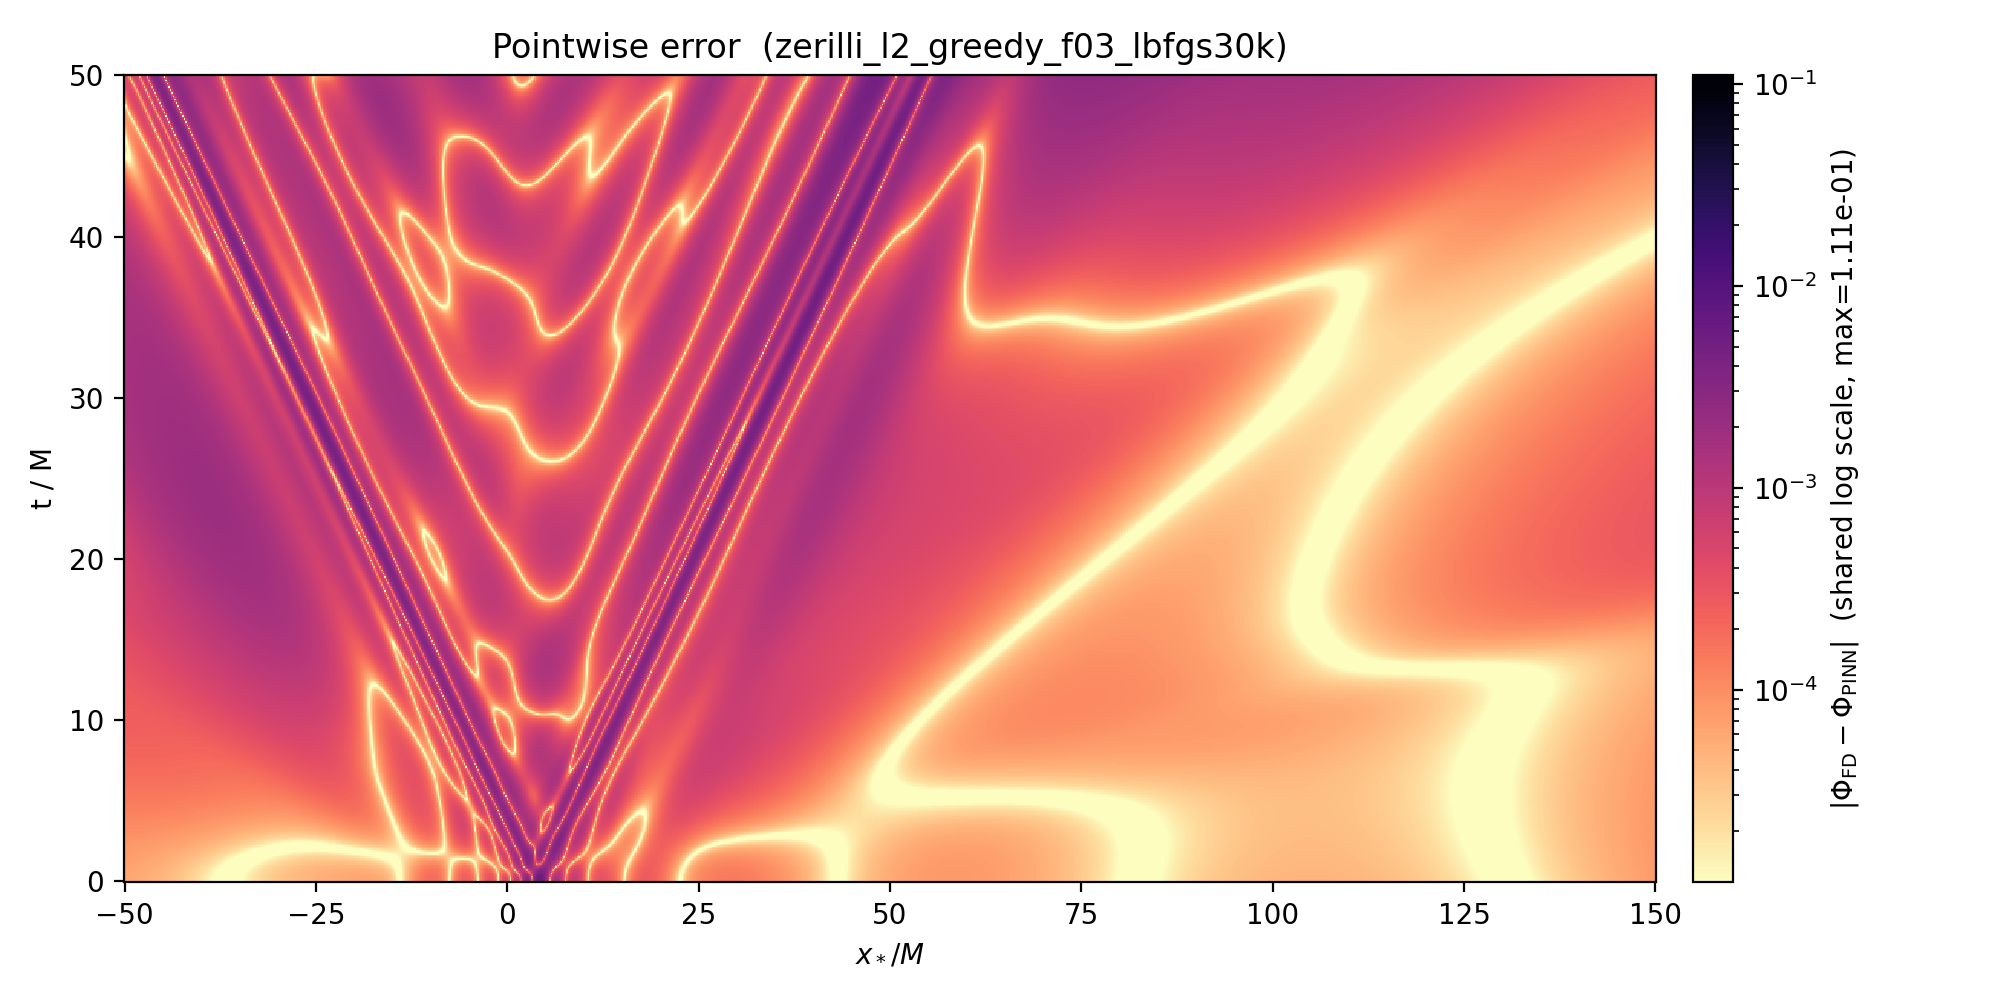
\includegraphics[width=0.92\textwidth]{../outputs/pinn/zerilli_l2_greedy_f03_lbfgs30k/error_heatmap.png}
\caption{Forward PINN global pointwise error. Heatmap of
$|\Phi_\theta - \Phi_{\mathrm{FD}}|$ on the full training domain
$x\in[-50,150]\,M$, $t\in[0,50]\,M$, confirming that the snapshot-time
bound of Fig.~\ref{fig:fwd-field} holds globally.}
\label{fig:fwd-heatmap}
\end{figure}

\begin{figure}[!htbp]
\centering
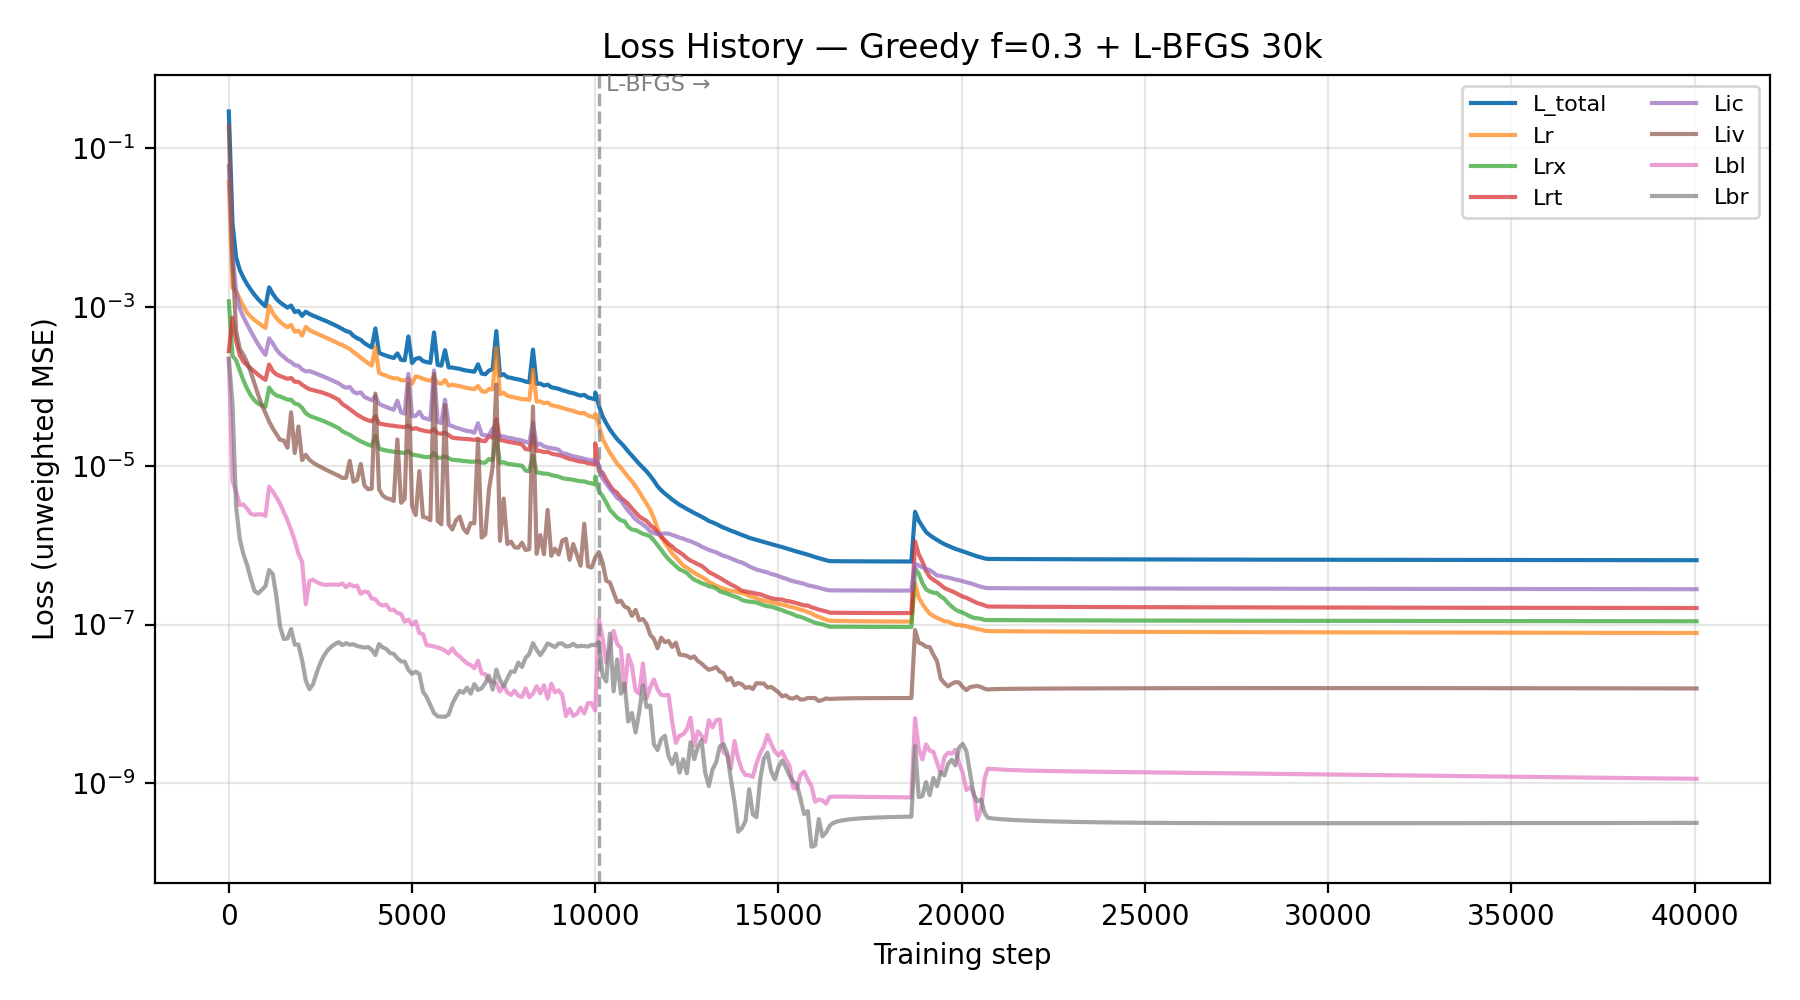
\includegraphics[width=0.85\textwidth]{../outputs/pinn/zerilli_l2_greedy_f03_lbfgs30k/loss.png}
\caption{Forward PINN training history. Total loss
$\mathcal{L}_{\mathrm{tot}}$ and the seven weighted components
($\mathcal{L}_{\mathrm{r}}$, $\mathcal{L}_{\mathrm{rx}}$,
$\mathcal{L}_{\mathrm{rt}}$, $\mathcal{L}_{\mathrm{ic}}$,
$\mathcal{L}_{\mathrm{iv}}$, $\mathcal{L}_{\mathrm{bl}}$,
$\mathcal{L}_{\mathrm{br}}$, weights as in
Sec.~\ref{sec:fwd-pinn}) versus iteration on a log--log axis. The
vertical marker at iteration $10{,}000$ separates the Adam phase
from the L-BFGS phase. The PDE-residual term
$\mathcal{L}_{\mathrm{r}}$ dominates throughout, with the IC and BC
terms below it by one to two orders of magnitude.}
\label{fig:fwd-loss}
\end{figure}

We apply the five extraction methods of Sec.~\ref{sec:qnm-methods}
to the time series $\Phi_\theta(\xq=10\,M,t)$ from the converged
forward PINN. The extracted ringdown, with its single-mode template
overlay, is shown in Fig.~\ref{fig:fwd-ringdown}; the primary
numbers from each method are collected in
Table~\ref{tab:fwd-qnm}, and the plateau diagnostics that justify
the M4 and M5 estimates are shown in Figs.~\ref{fig:fwd-plateau-m4} and~\ref{fig:fwd-plateau-m5}.

\begin{figure}[!htbp]
\centering
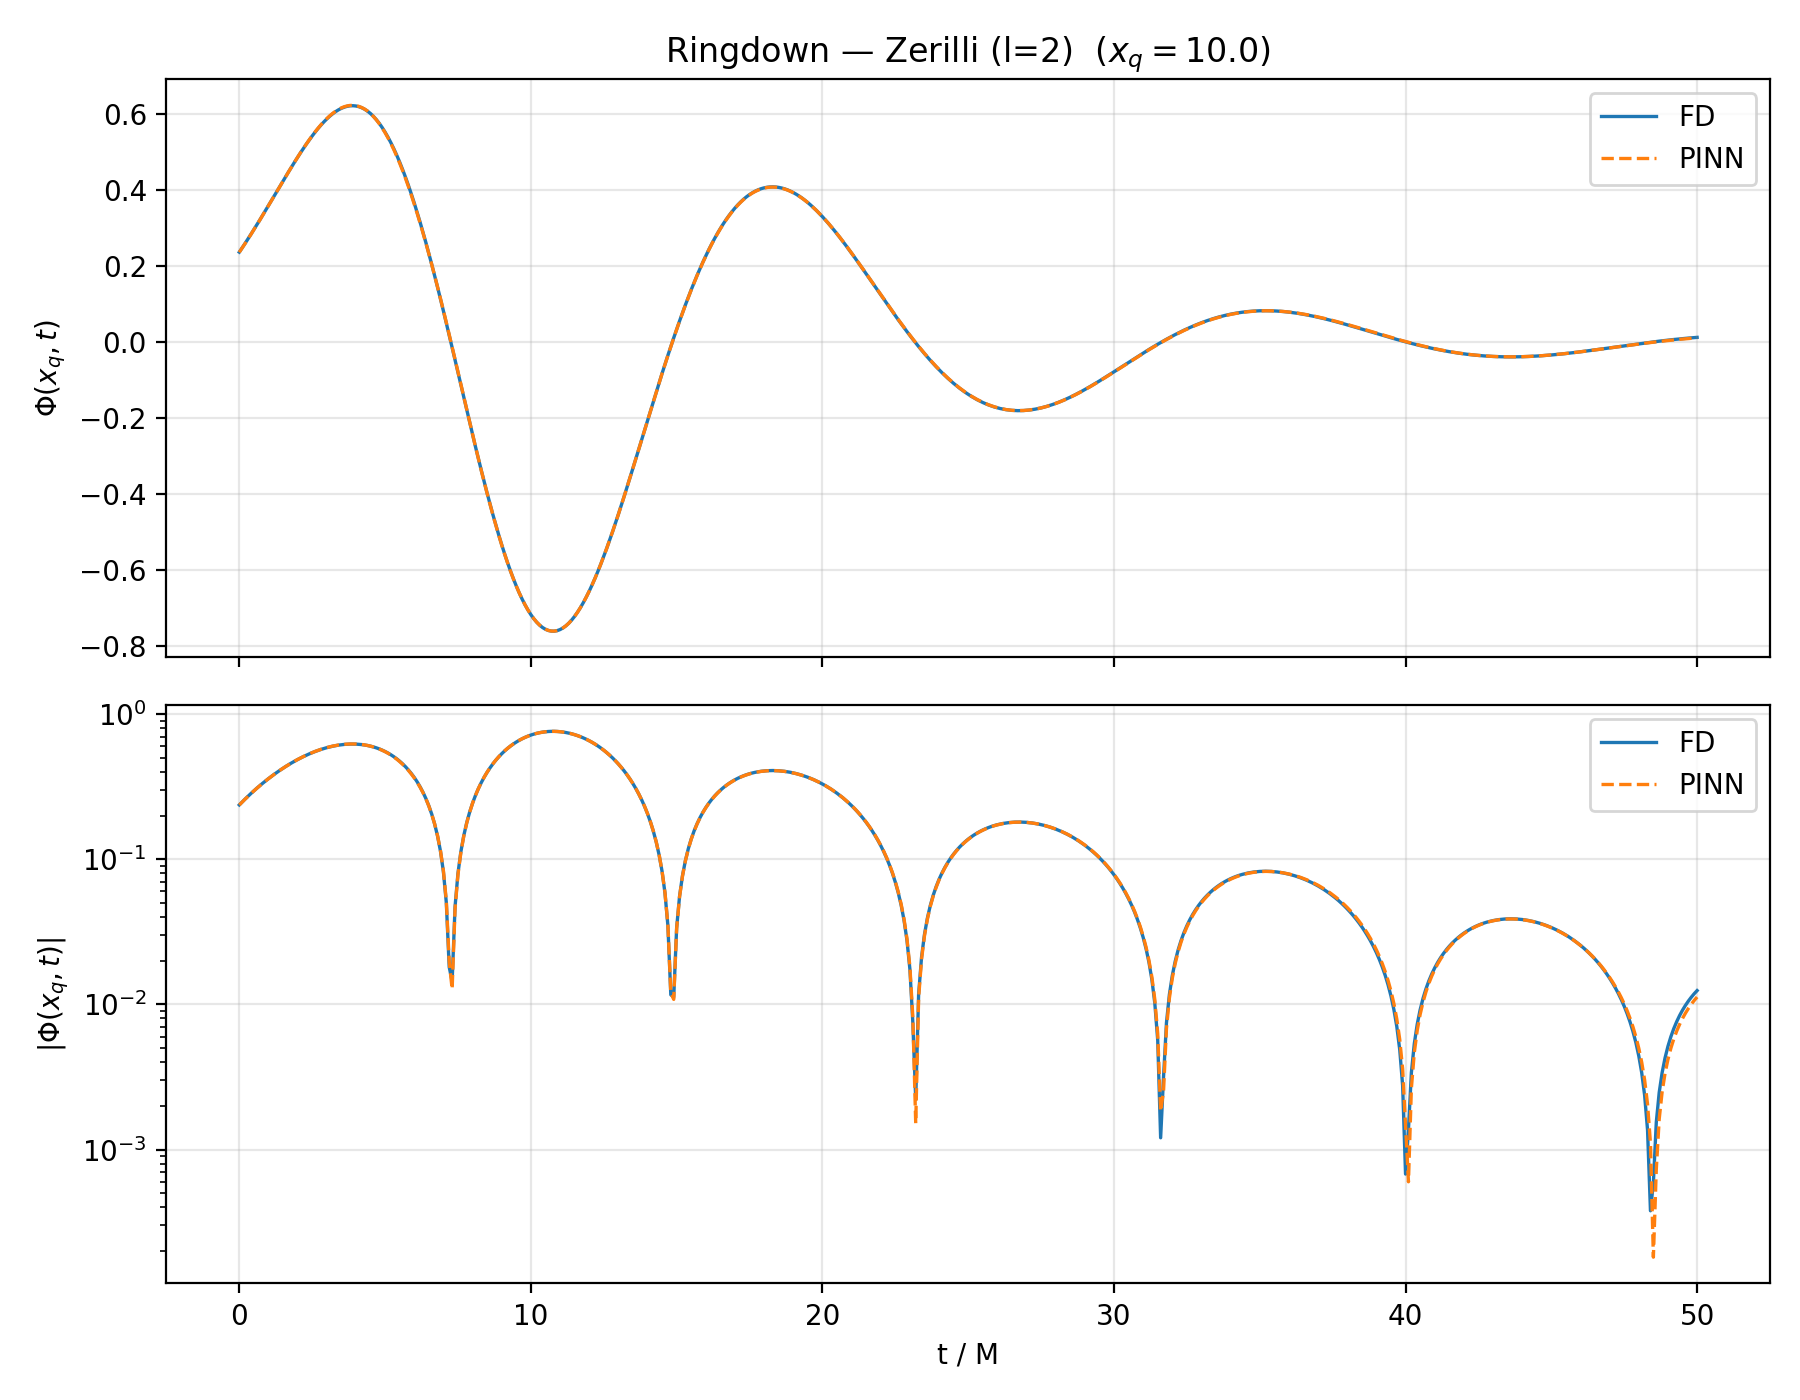
\includegraphics[width=0.85\textwidth]{../outputs/pinn/zerilli_l2_greedy_f03_lbfgs30k/ringdown_overlay.png}\\[0.6em]
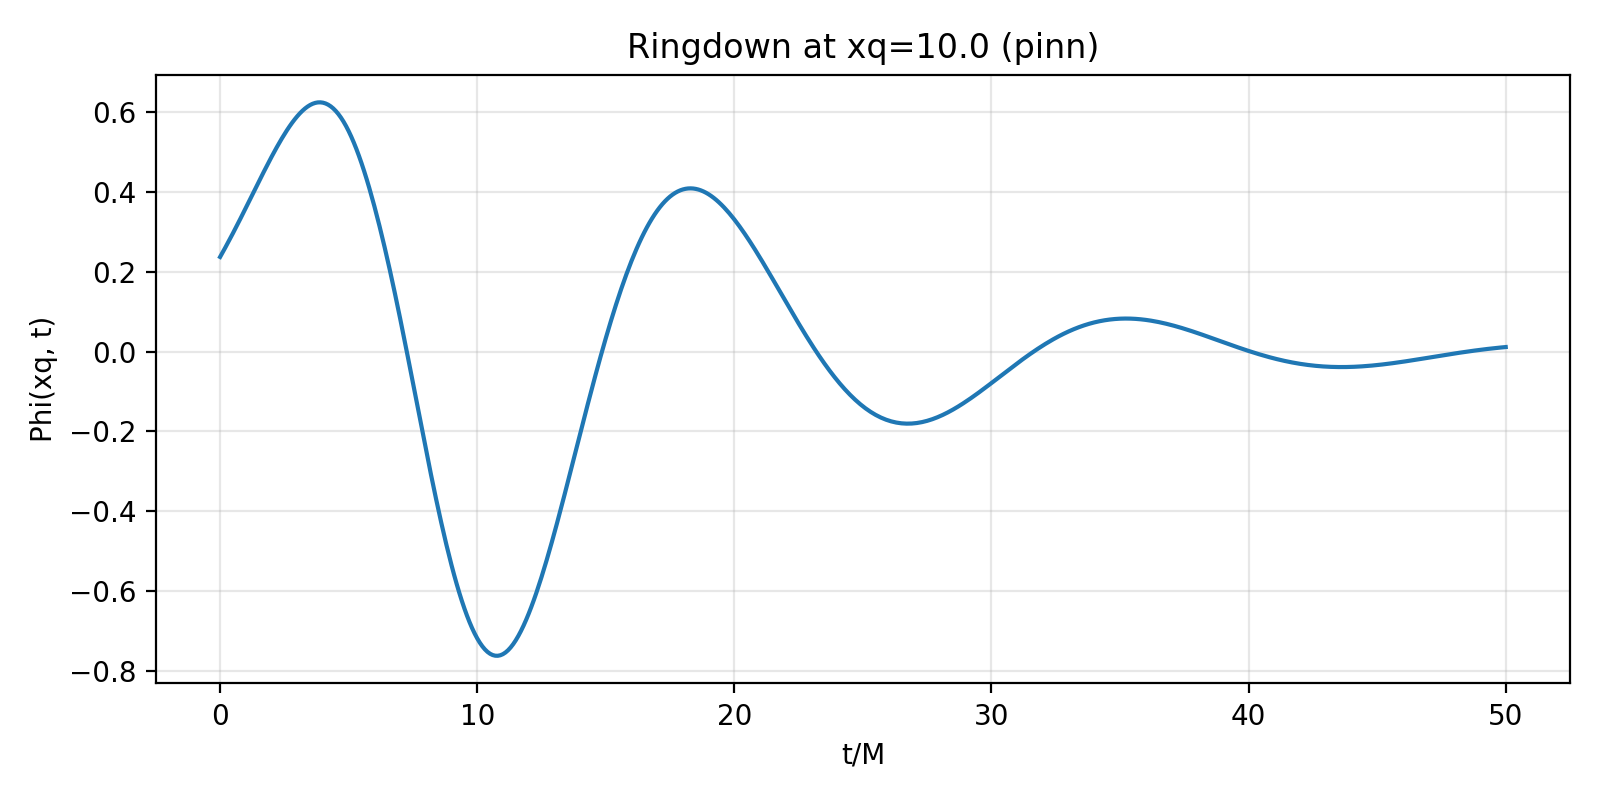
\includegraphics[width=0.85\textwidth]{../outputs/qnm/zerilli_l2_greedy_f03_lbfgs30k/pinn_ringdown.png}
\caption{Forward PINN ringdown at $\xq = 10\,M$. Top two panels:
$\Phi_\theta(\xq,t)$ from the forward PINN overlaid on the FD
reference on linear (upper) and logarithmic (lower) vertical
scales, showing the prompt burst followed by the
exponentially-damped sinusoidal ringdown. Bottom: the same
time series isolated from $\Phi_\theta$, on which the five
extraction methods of Sec.~\ref{sec:qnm-methods} are applied to
produce the entries of Table~\ref{tab:fwd-qnm}.}
\label{fig:fwd-ringdown}
\end{figure}

\begin{table}[!htbp]
\centering
\caption{Forward PINN QNM extraction. Reference values are the
Leaver continued-fraction Schwarzschild $\ell = 2$ fundamental
$M\omega_0 = 0.3737$, $\tau_0/M = 11.241$. ``Wide'' window
denotes $[10,50]\,M$; M2 on plateau denotes M2 evaluated on the
$[t_0^{\min},50]\,M$ window with $t_0^{\min}$ taken as the lower
edge of the M4 plateau. M4 and M5 quote
plateau-mean $\pm$ plateau standard deviation across the
contiguous block of fit windows minimising the combined relative
scatter (Algorithm~\ref{alg:m4} and Sec.~\ref{sec:plateau}).
Bold entries are the primary values under the reporting
convention of Sec.~\ref{sec:reporting}.}
\label{tab:fwd-qnm}
\footnotesize
\setlength{\tabcolsep}{4pt}
\renewcommand{\arraystretch}{1.05}
\begin{tabular}{@{}lccccl@{}}
\toprule
Method & $M\omega$ & $\omega$ err & $\tau/M$ & $\tau$ err & Window or plateau \\
\midrule
M1 (FFT $+$ log-line)        & $0.3712$  & $0.68\%$  & $10.92$ & $2.83\%$ & $[10,\,50]\,M$ \\
M2 (NLS, wide)               & $0.3794$  & $1.54\%$  & $11.464$ & $\mathbf{1.99\%}$ & $[10,\,50]\,M$ \\
M2 (NLS on M4 plateau)       & $0.3749$  & $0.31\%$  & $10.41$ & $7.38\%$ & $[14,\,50]\,M$ \\
M3 (ESPRIT, $K=6$)           & $0.4829$  & $29.2\%$  & $7.84$  & $30.3\%$ & $[10,\,50]\,M$ \\
M4 (1-D plateau)             & $0.37359{\pm}2{\times}10^{-4}$ & $\mathbf{0.029\%}$ & $10.94{\pm}0.02$ & $2.65\%$ & $t_0\in[14,21]M$, $\tend{=}50M$ \\
M5 (2-D plateau)             & $0.3728{\pm}8{\times}10^{-4}$ & $0.23\%$ & $10.80{\pm}0.12$ & $3.91\%$ & $t_0\in[10,16.7]M$, $\tend\in[42,50]M$ \\
\bottomrule
\end{tabular}
\end{table}

\begin{figure}[!htbp]
\centering
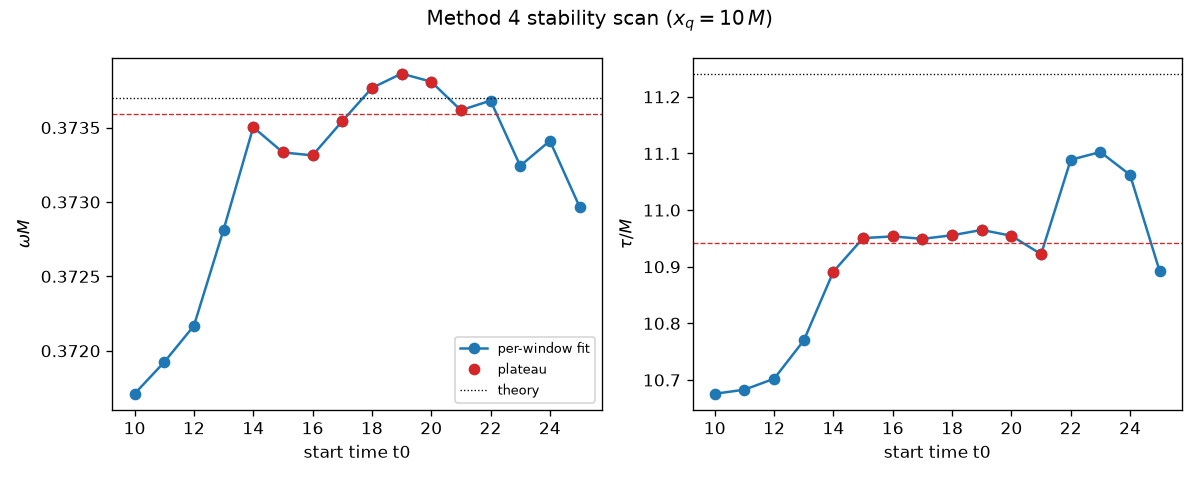
\includegraphics[width=0.95\textwidth]{../outputs/qnm/zerilli_l2_greedy_f03_lbfgs30k/pinn_method4_stability.png}
\caption{M4 plateau diagnostic for the forward PINN.
$(\omega_0,\tau_0)$ as a function of the start time $t_0$ on
$[10,25]\,M$ at fixed $\tend = 50\,M$, with the eight-window
plateau block ($t_0\in[14,21]\,M$) shaded.}
\label{fig:fwd-plateau-m4}
\end{figure}

\begin{figure}[!htbp]
\centering
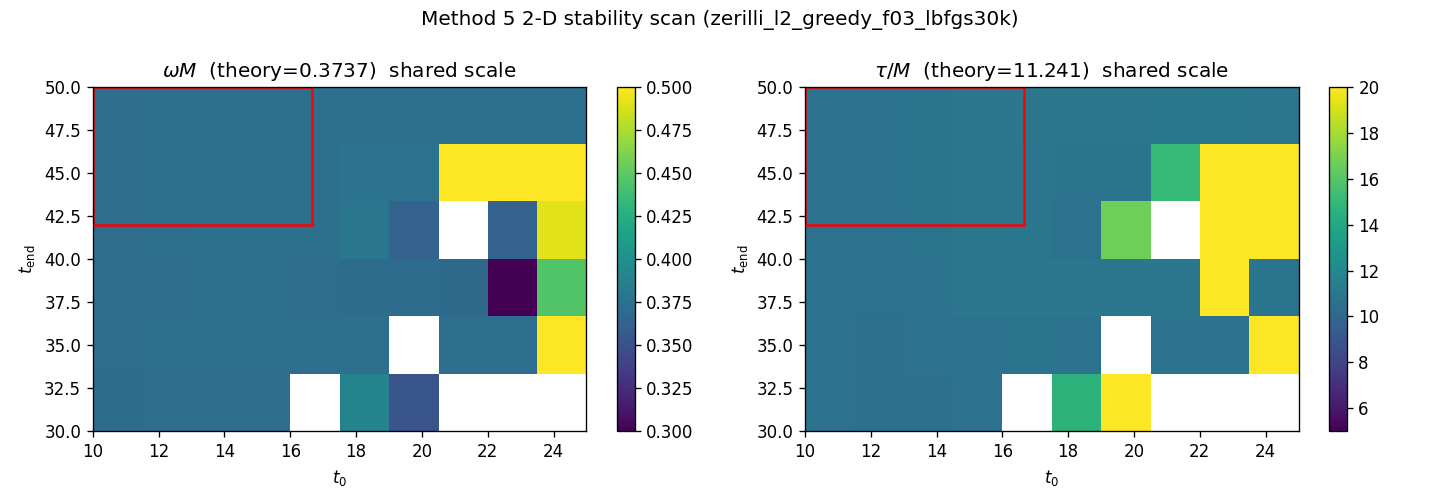
\includegraphics[width=0.85\textwidth,keepaspectratio]{../outputs/qnm/zerilli_l2_greedy_f03_lbfgs30k/pinn_method5_2d_heatmap.png}
\caption{M5 plateau diagnostic for the forward PINN. Heatmap of
the absolute deviation of the M2 estimate from the plateau median
on the $(t_0,\tend)$ grid (capped at $5\%$); the contiguous
$5\times 3$ plateau rectangle is outlined in red. Top:
$\omega_0$. Bottom: $\tau_0$. Annotations report the in-block
relative scatter (the quantity the plateau rule minimises) and
the bias of the plateau mean from the Leaver value.}
\label{fig:fwd-plateau-m5}
\end{figure}

Two points stand out. The M4 plateau estimate reaches
$0.029\%$ in $\omega$, an order of magnitude tighter than any
single-window method, while M2 on the M4 plateau window
sharpens $\omega$ but degrades $\tau$, so $\omega$ and $\tau$
are taken from different estimators under the selection rule of
Sec.~\ref{sec:reporting}.
M3 returns frequencies at machine-precision amplitudes and is
quoted in Appendix~\ref{app:esprit} only.

\paragraph{Error budget.} The two measured contributions to
the frequency error rank as follows: the M4 bias against the
Leaver value is $1.1\times 10^{-4}$ in $M\omega$ ($0.029\%$),
and the fit-window systematic is $\sigma_\omega = 2\times 10^{-4}$
($0.054\%$; a lower bound, Sec.~\ref{sec:plateau}). The
frequency measurement is therefore
window-limited, not field-limited. For the
M4 damping time the ordering reverses: its plateau scatter
$\sigma_\tau/\tau \approx 0.2\%$ sits against a $2.65\%$ bias, so
the M4 $\tau$ is field- and template-limited rather than
window-limited; the Leaver-closest damping time is instead M2 on
the wide window ($1.99\%$), the value reported in
Table~\ref{tab:results-summary}.

\FloatBarrier

% --------------------------------------------------------------
\subsection{Hybrid coarse-FD + neural-residual surrogate}
\label{sec:res-hyb}

The final model asks how much of the fine solver's
accuracy can be recovered from a classical solve at $1/64$ of
its cost. The hybrid surrogate of Sec.~\ref{sec:hyb-method}
keeps a coarse-grid FD solve to carry the wave propagation and
asks the
network only
for the pointwise residual against the fine-grid solution of
the same problem. It is evaluated on the canonical draw
$(M,x_{0},\sigma) = (1,4,5)$ and on a $100$-BH in-distribution
Sobol test set (drawn from the hybrid's own training box,
Sec.~\ref{sec:hyb-method}), at coarsening factor $k = 4$ with
the label-free Richardson training target of
Eqs.~\eqref{eq:hyb-richardson}--\eqref{eq:hyb-residual};
extraction is at the common observer $\xq = 10\,M$ shared with
the PINNs, over the model's full $[10,100]\,M$ evolution. The $k = 4$ prior is deliberately weak ($4.93\%$ relative
$L^{2}$ on the canonical draw), leaving a large but
spatially-localised dispersion error for the gated network to
repair.

\paragraph{Field accuracy on the canonical BH.} The hybrid
reproduces the fine FD reference with gridwise
$\mathrm{RMSD} = 6.28\times 10^{-4}$, against
$6.95\times 10^{-3}$ for the quintic-spline upsample of the
coarse solve alone (henceforth the \emph{coarse-up baseline}):
the gated residual suppresses
the coarse-prior discretisation error by a factor of $11.1$
(equivalently $0.445\%$ versus $4.93\%$ in relative $L^{2}$).
The residual is concentrated on the outgoing wavefronts where
the coarse prior dephases (Fig.~\ref{fig:hyb-snapshots}); the
global error maps (Figs.~\ref{fig:hyb-heatmap}
and~\ref{fig:hyb-heatmap-base}) show the hybrid suppressing
the baseline's dispersion characteristics by roughly an order
of magnitude while leaving the smooth interior and causal
exterior at the prior --- the correction lands exactly where
the gate directs it.

\begin{figure}[!htbp]
\centering
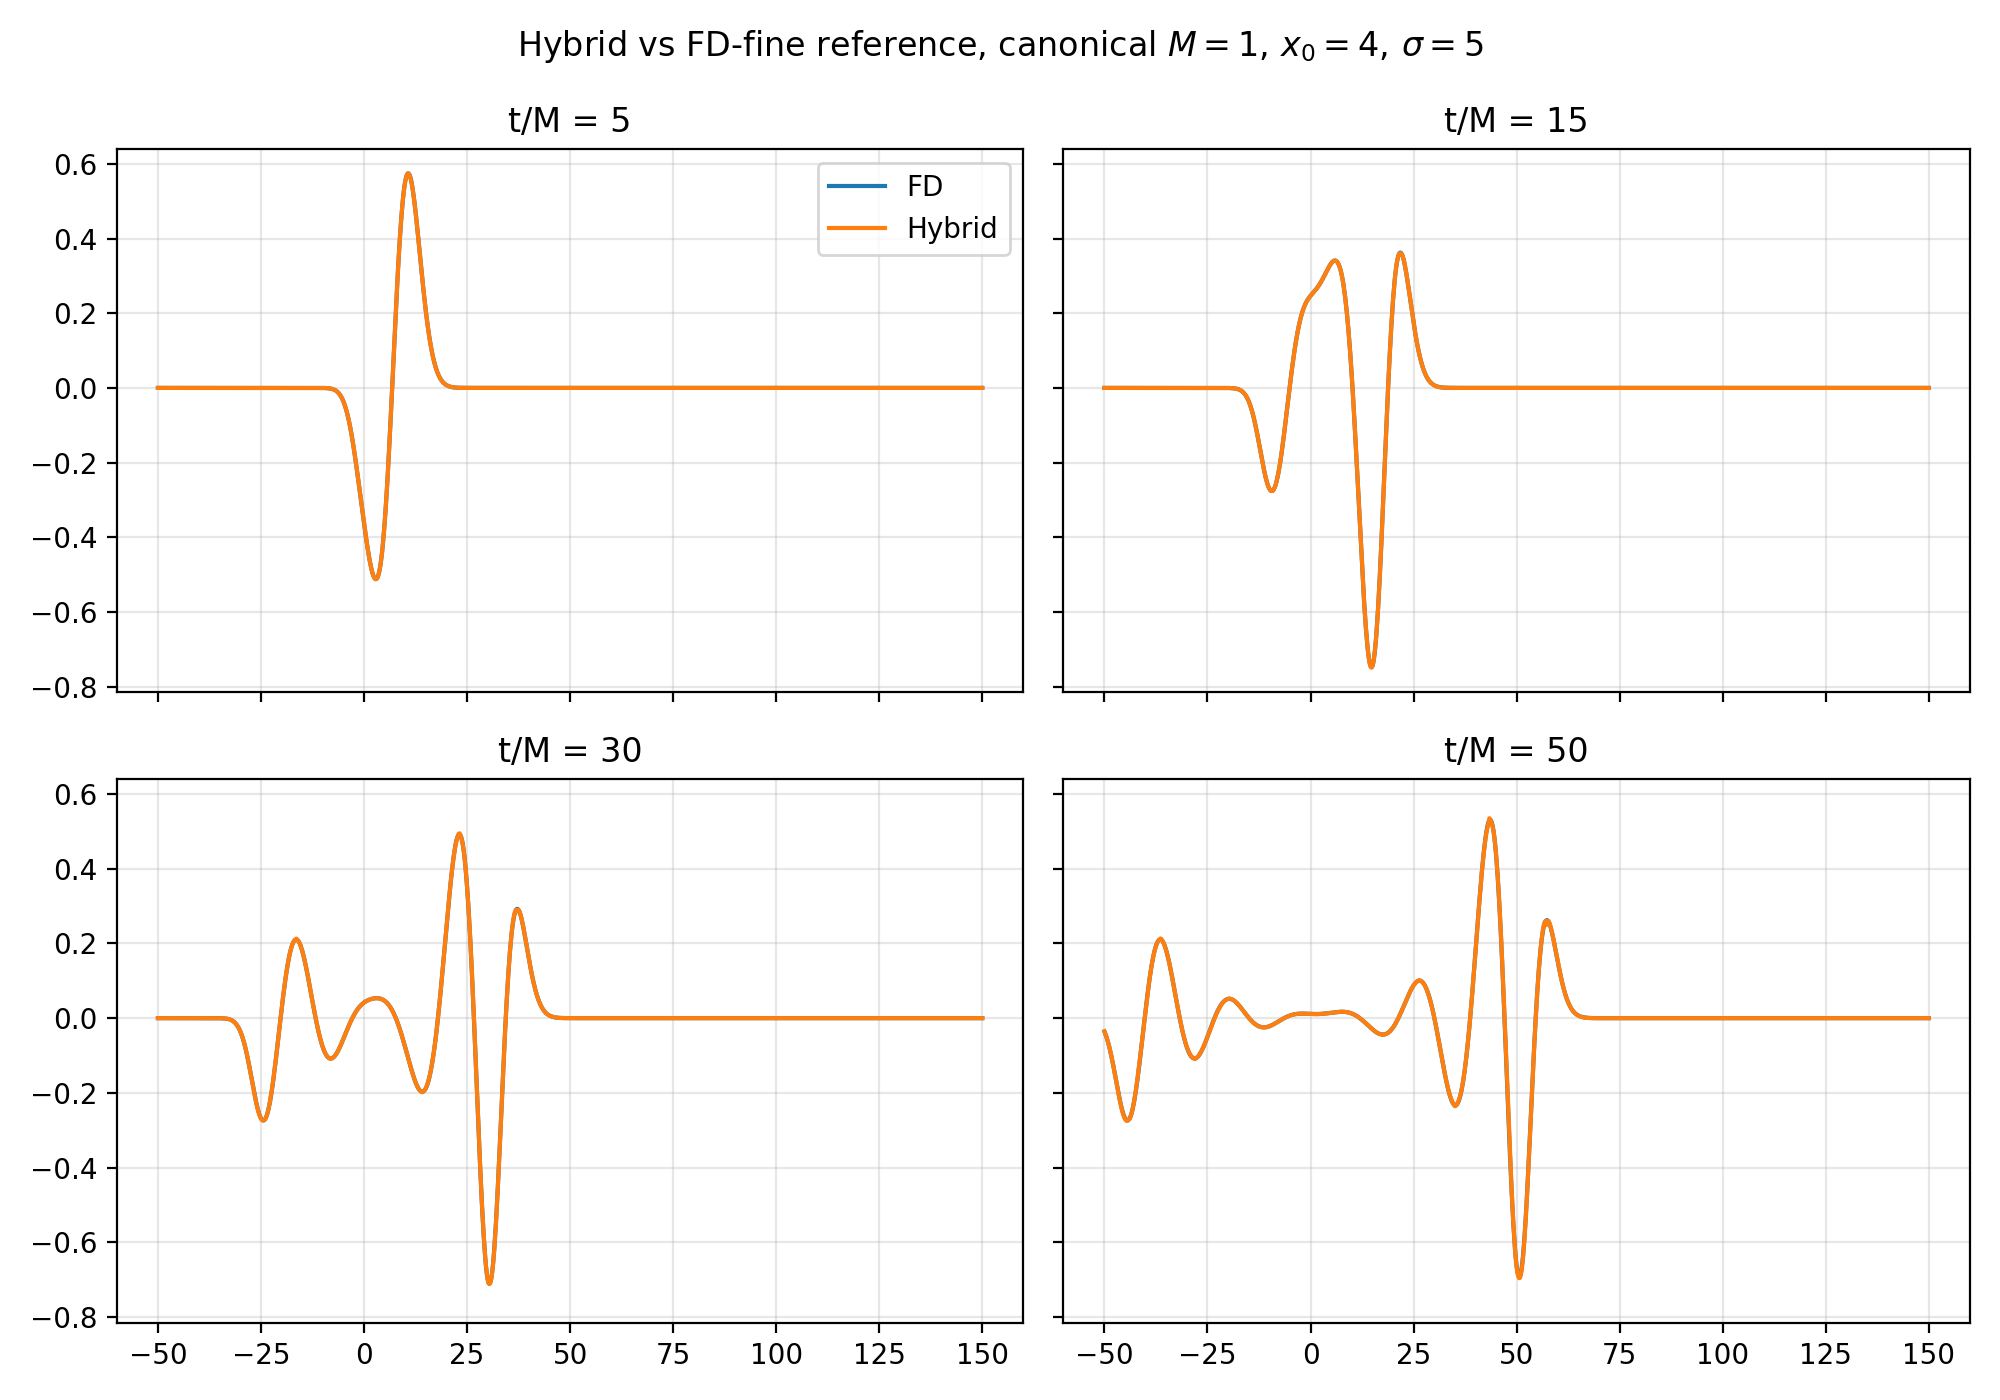
\includegraphics[width=0.82\textwidth]{../outputs/hybrid/fno_sw_gate_s1em3/figs/hybrid_snapshots.png}\\[0.4em]
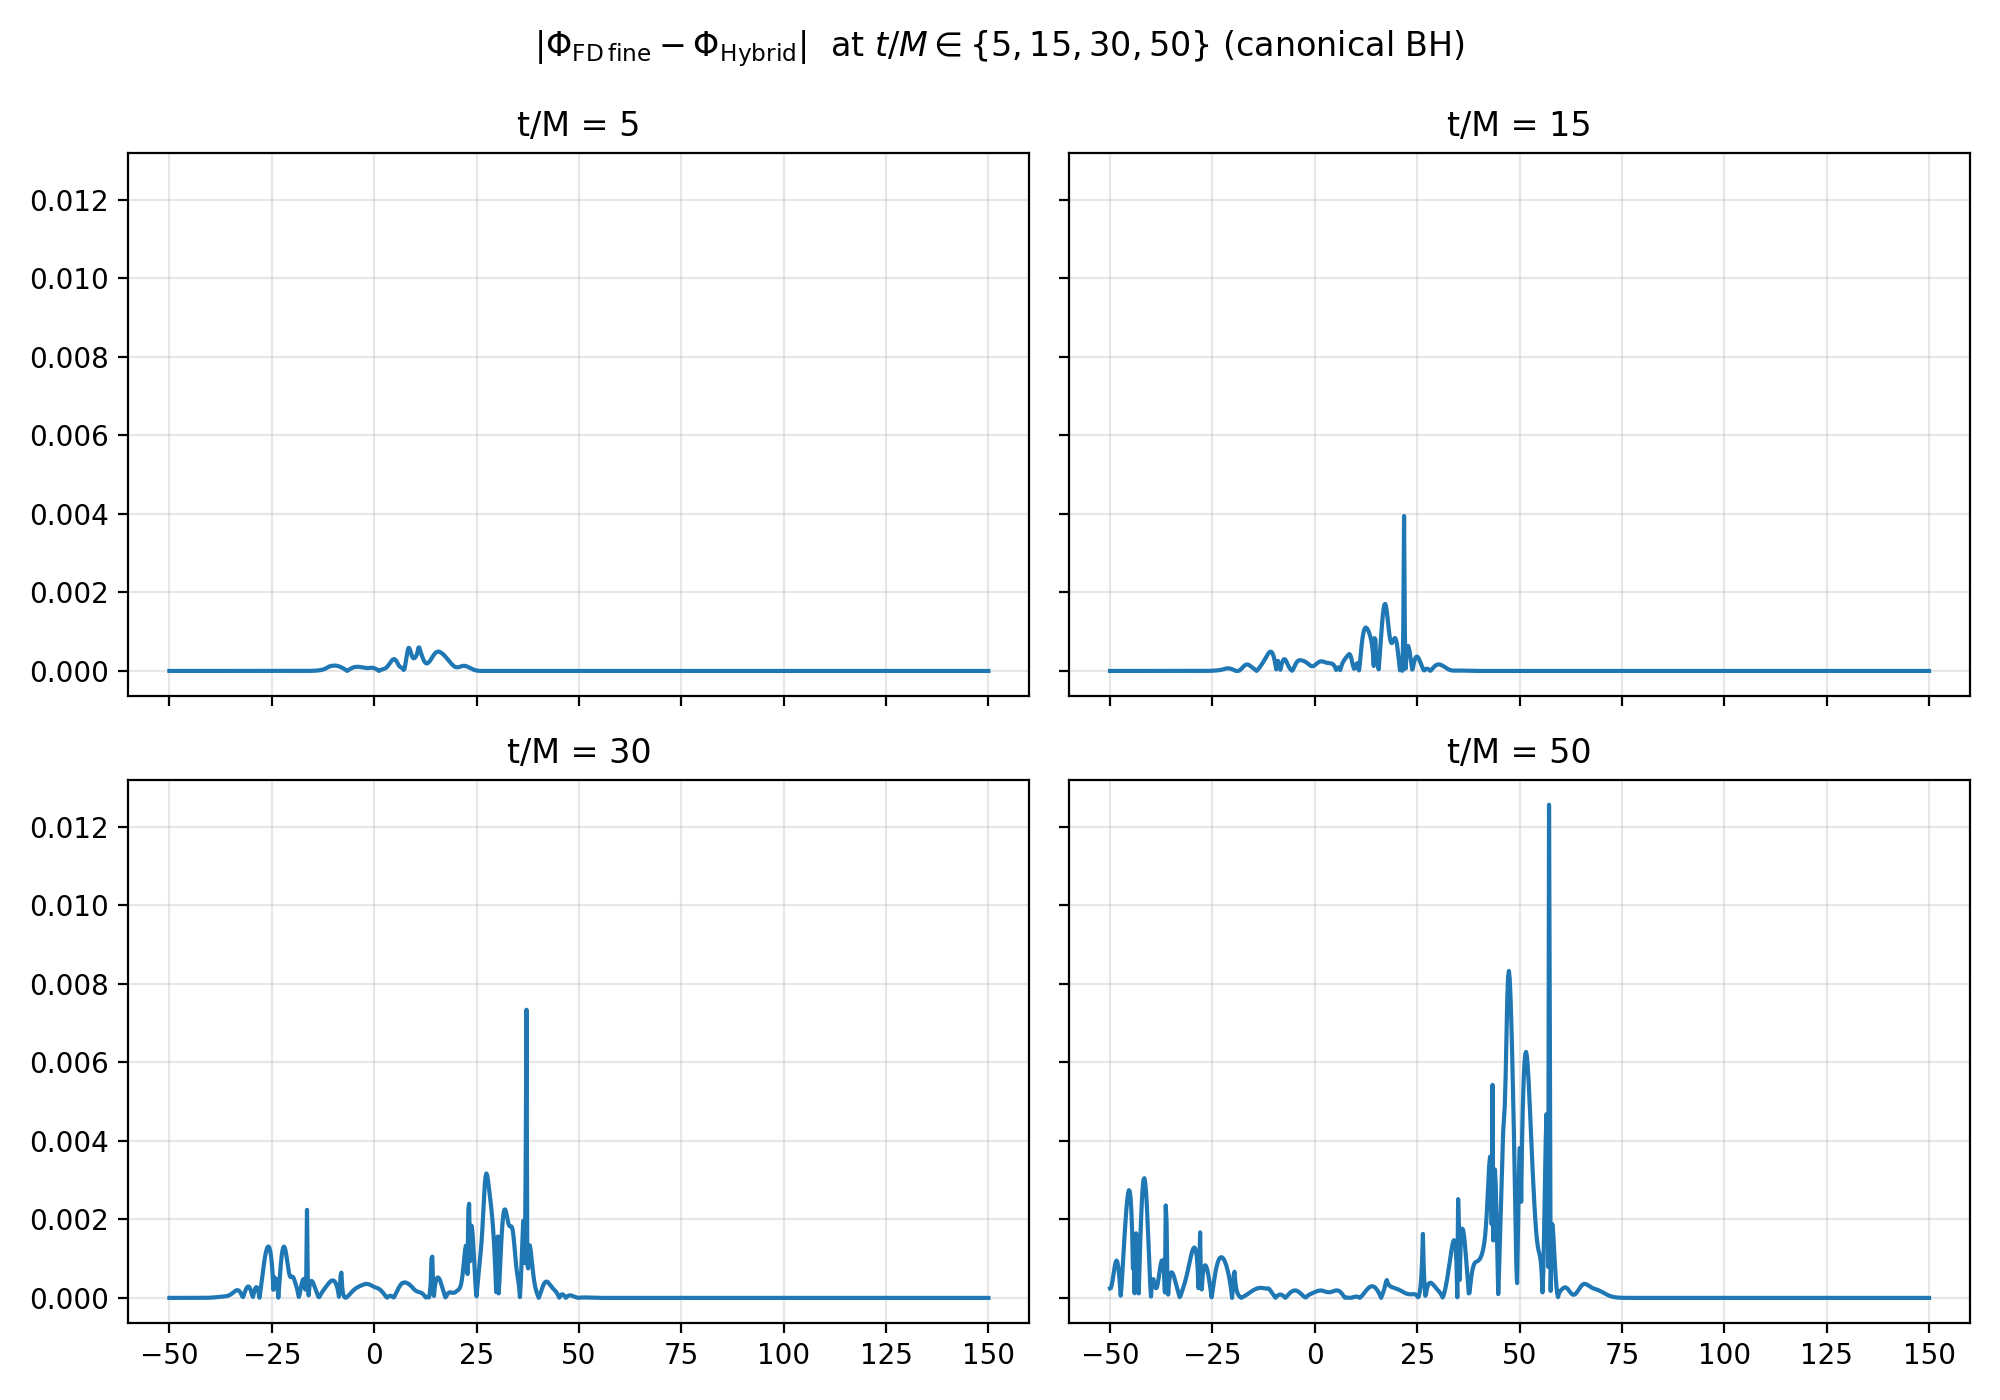
\includegraphics[width=0.82\textwidth]{../outputs/hybrid/fno_sw_gate_s1em3/figs/hybrid_abs_diff_snapshots.png}
\caption{Hybrid prediction versus fine FD reference on the
canonical BH at four snapshot times. Top: $\Phi(x,t)$ at
$t/M \in \{5, 15, 30, 50\}$, with the fine FD reference (blue)
and the hybrid prediction (orange) overlaid; the two curves
are visually indistinguishable on this scale. Bottom: pointwise
$|\Phi^{\mathrm{f}} - \Phi^{\mathrm{hyb}}|$ at the same four
times, concentrated on the outgoing wavefronts and near-zero
across the smooth interior and the causal exterior.}
\label{fig:hyb-snapshots}
\end{figure}

\begin{figure}[!htbp]
\centering
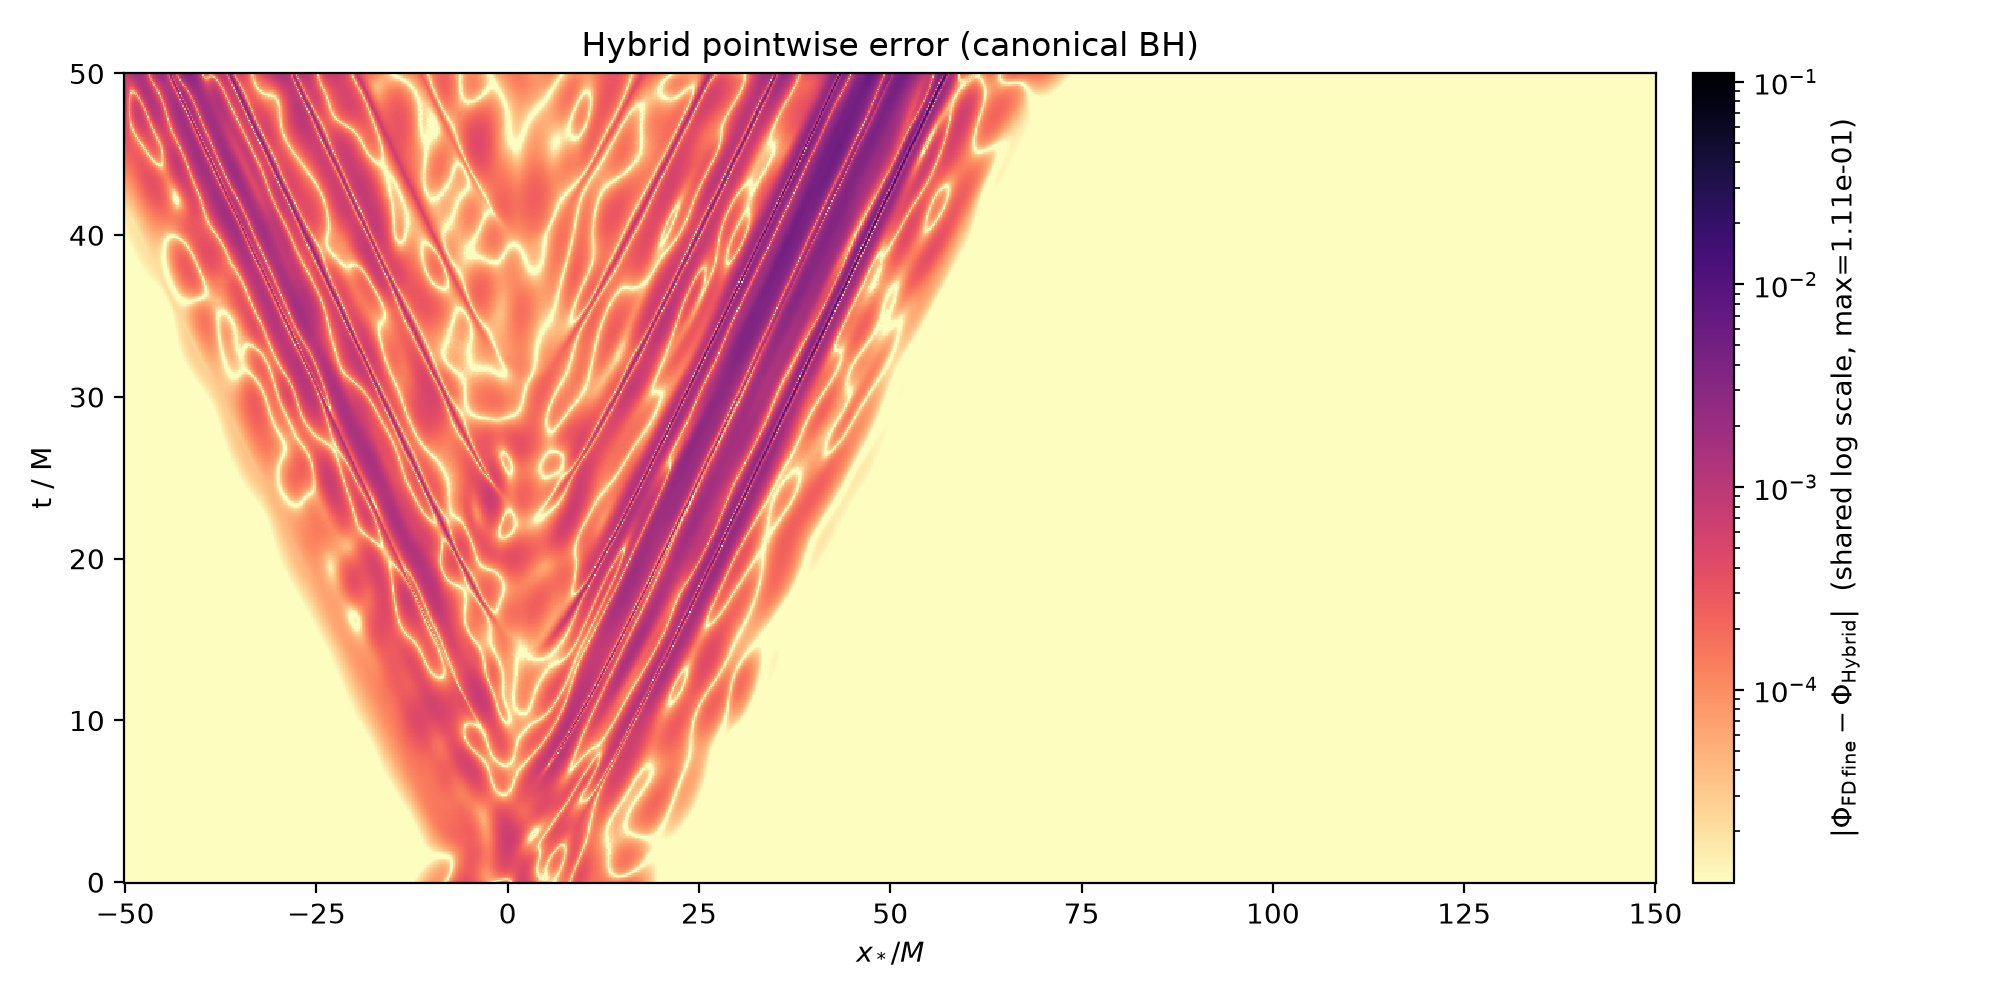
\includegraphics[width=0.92\textwidth]{../outputs/hybrid/fno_sw_gate_s1em3/figs/hybrid_pointwise_error.png}
\caption{Hybrid surrogate global pointwise error on the
canonical BH. Heatmap of
$|\Phi^{\mathrm{f}} - \Phi^{\mathrm{hyb}}|$ on
$x \in [-50, 150]\,M$, $t \in [0, 50]\,M$ (the full hybrid
training and evaluation window), plotted on a
logarithmic $\mathrm{magma\_r}$ colour
scale. The residual structure is confined by the
gradient gate to the prompt-burst region $t \lesssim 5\,M$ and
the outgoing wavefronts; the smooth interior and causal
exterior are left at the prior. Compare with the
coarse-up baseline error on the same
colour scale in Fig.~\ref{fig:hyb-heatmap-base}.}
\label{fig:hyb-heatmap}
\end{figure}

\begin{figure}[!htbp]
\centering
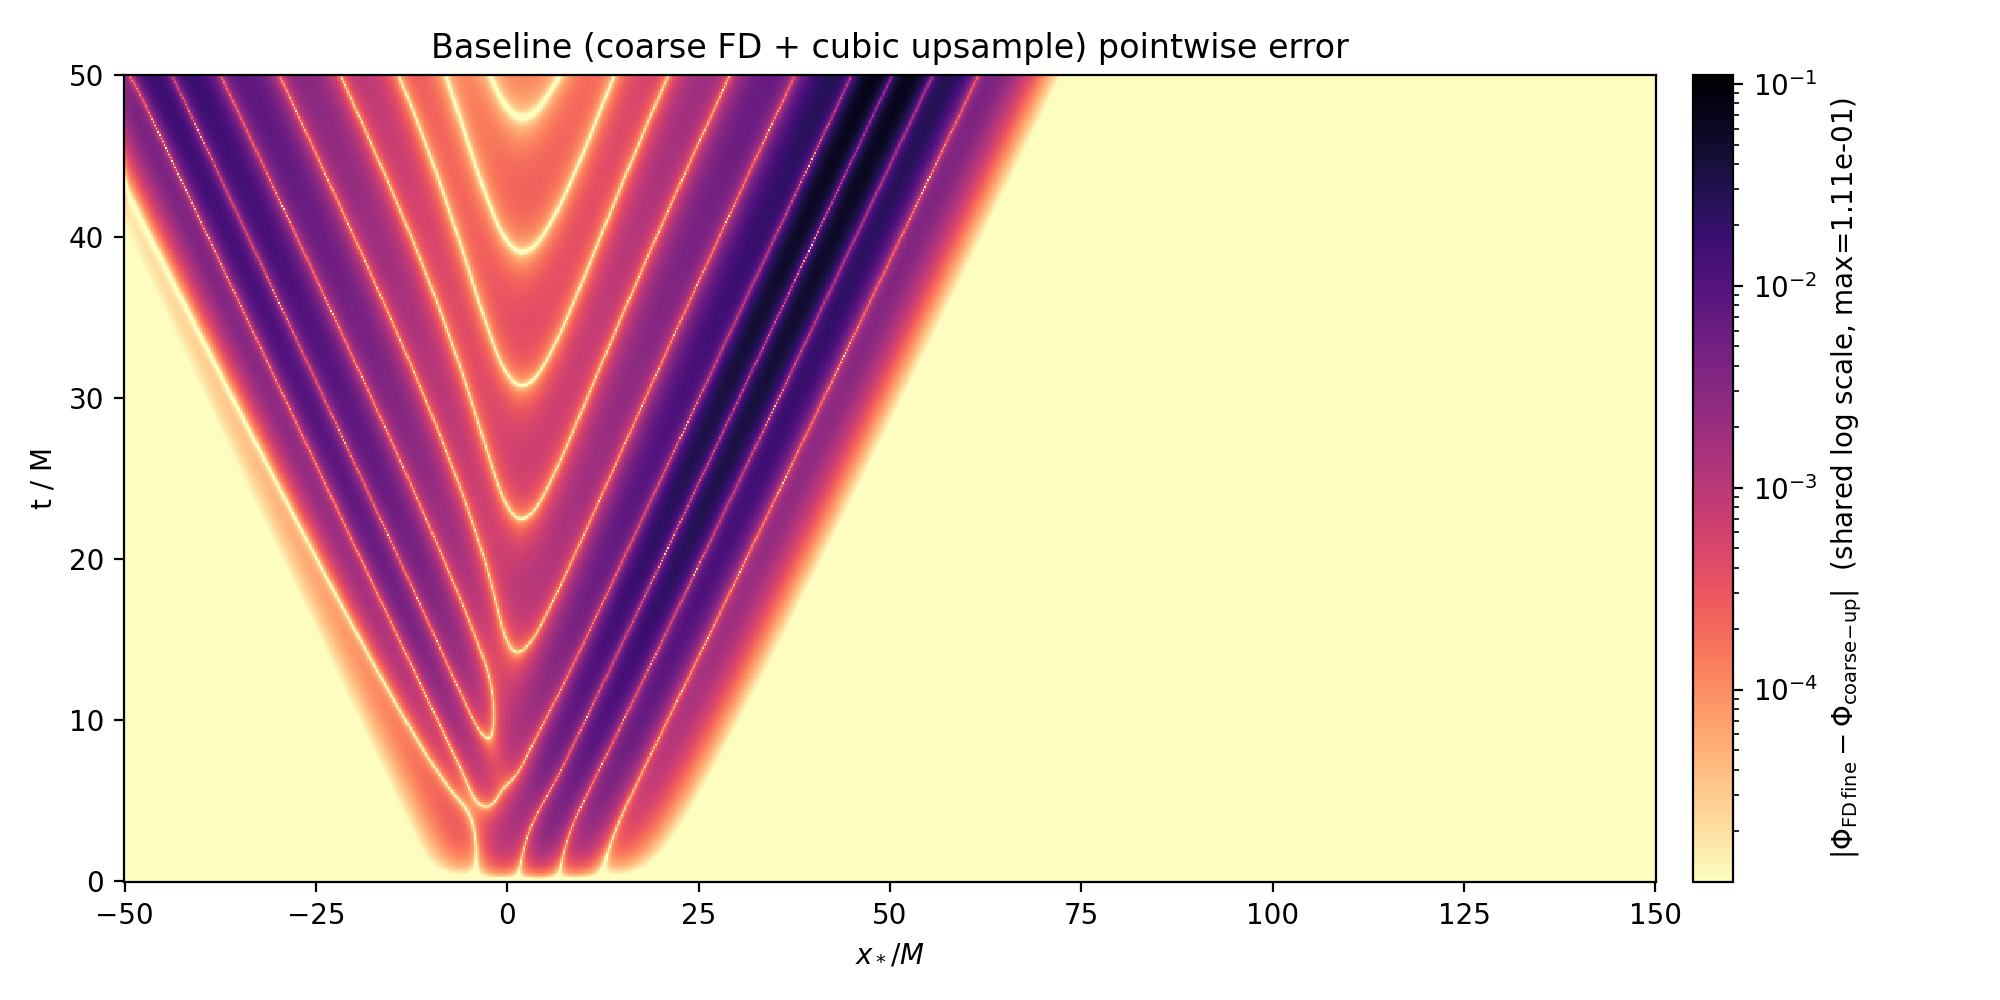
\includegraphics[width=0.92\textwidth]{../outputs/hybrid/fno_sw_gate_s1em3/figs/hybrid_pointwise_error_baseline.png}
\caption{Coarse-up baseline pointwise error on the canonical
BH, plotted on the same shared colour scale as
Fig.~\ref{fig:hyb-heatmap}. The second-order dispersion
signature of the under-resolved $k = 4$ coarse prior plus
quintic upsampling is visible as narrow characteristics tracing
the outgoing-wave caustics; compare the hybrid map of
Fig.~\ref{fig:hyb-heatmap} on the same scale.}
\label{fig:hyb-heatmap-base}
\end{figure}

\paragraph{The gradient gate.} The gate of
Eq.~\eqref{eq:hyb-gate} rests on the hypothesis that the
coarse-prior error is large exactly where the prior gradient
is large; the per-cell scatter on the canonical BH confirms
this with a log--log Pearson correlation of $r = 0.917$, and a
decile stratification shows the hybrid's gain following the
gate --- a factor $14.1$ error reduction in the top gradient
decile, declining monotonically to unity below the median
(Appendix~\ref{app:supp-gate}). The gate scale $s = 10^{-3}$
is derived from the prior gradient distribution alone and sits
within $2\%$ of the field-RMSD optimum
(App.~\ref{app:gate-scale}). The gate also protects the
regions the prior already resolves: over the $60.5\%$ of the
domain with prior error below $10^{-5}$, spurious network
output is held at the $10^{-6}$ level, so the global-field
gain does not pollute the QNM-bearing late-time tail.

\paragraph{Population field accuracy.} Averaged over the 100-BH
in-distribution test set, the gridwise field MSE is
$9.38\times 10^{-7}$ for the hybrid and $7.76\times 10^{-5}$
for the coarse-up baseline, a factor-of-$82$ reduction
($0.648\%$ vs $6.11\%$ relative $L^{2}$) --- consistent across
the whole training distribution rather than an artefact of the
canonical draw.

\begin{figure}[!htbp]
\centering
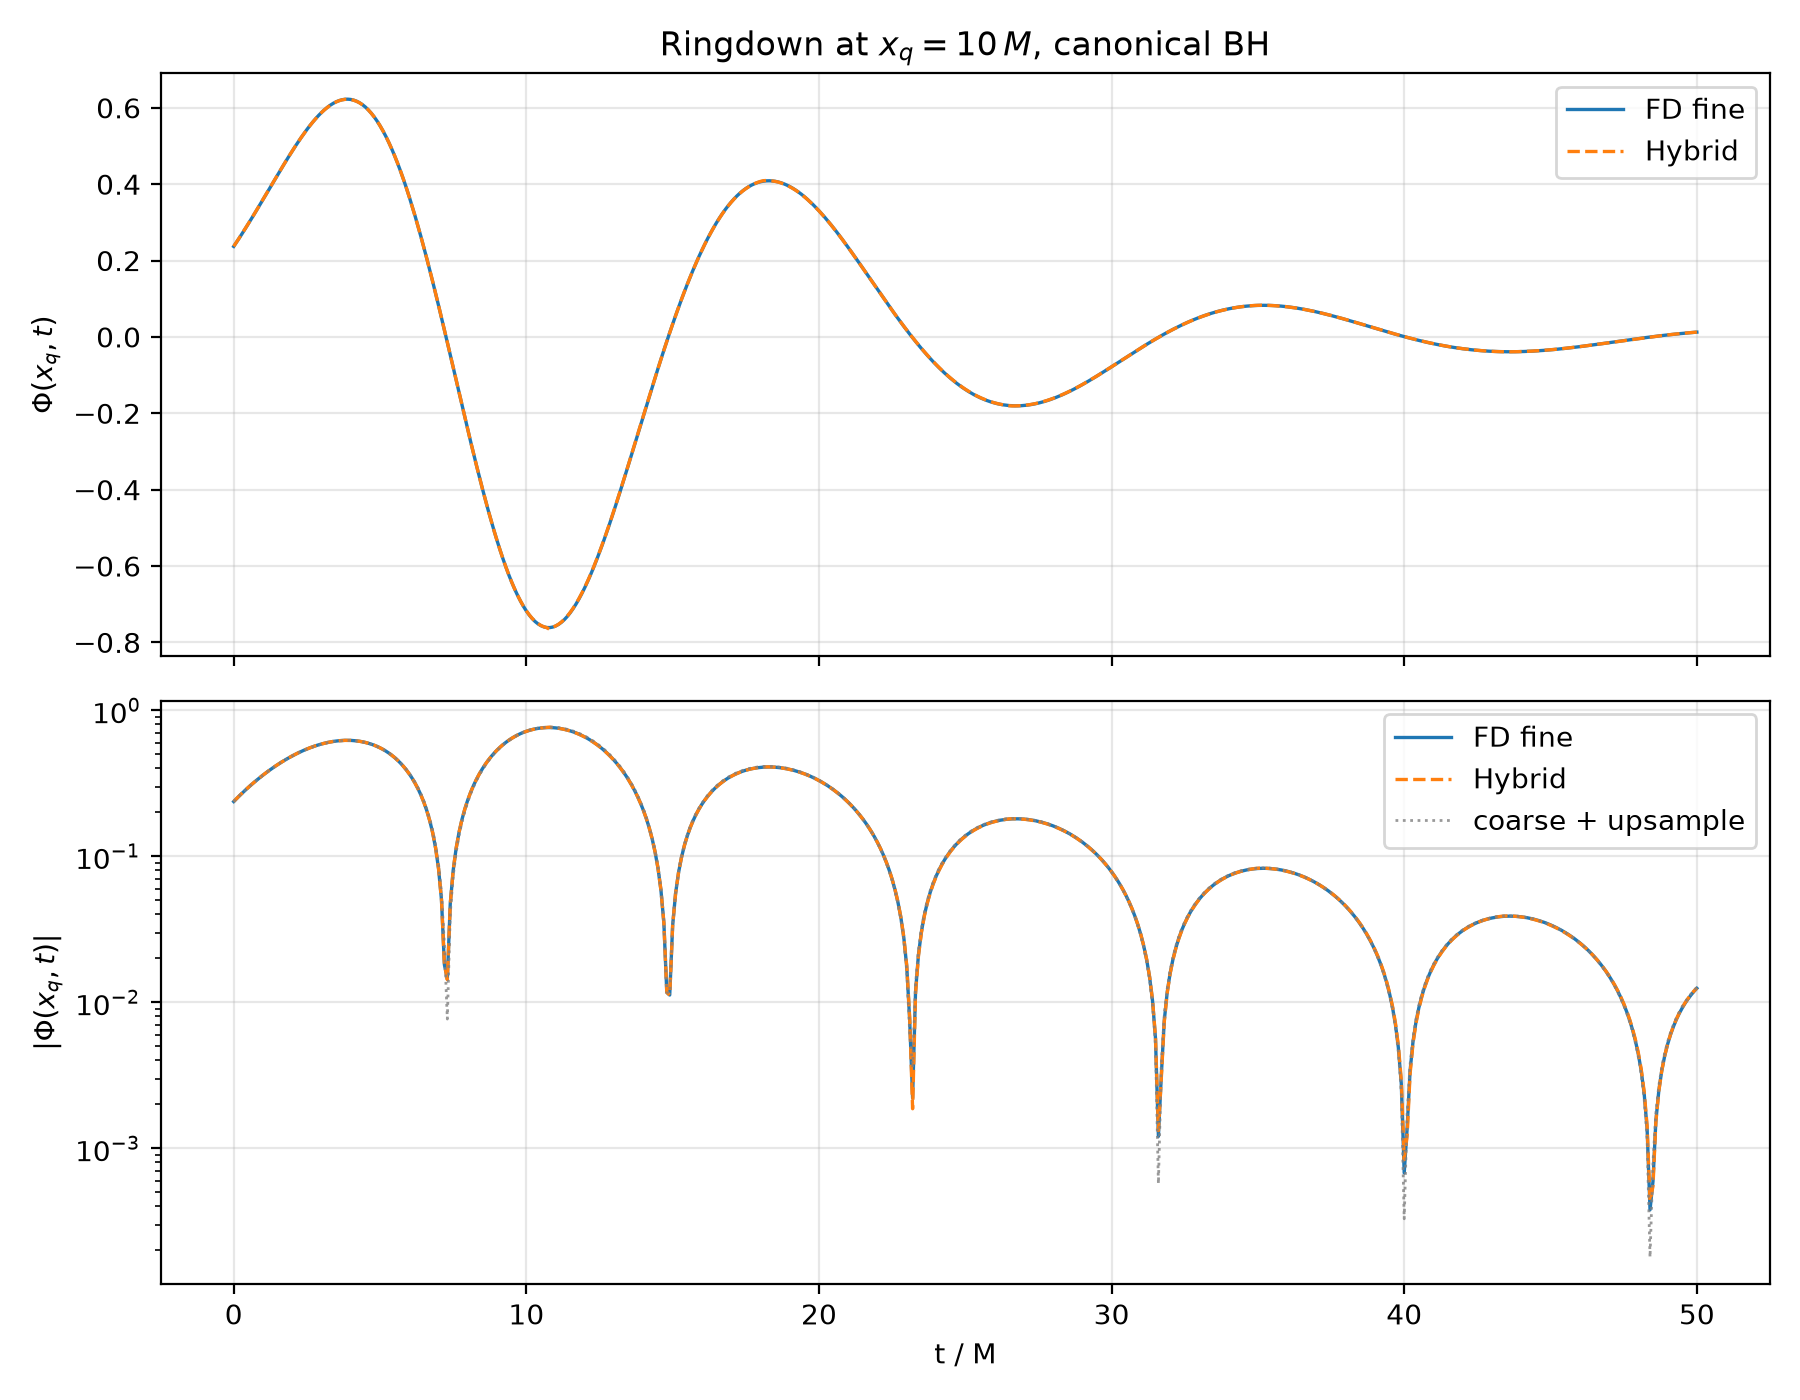
\includegraphics[width=0.80\textwidth]{../outputs/hybrid/fno_sw_gate_s1em3/figs/hybrid_ringdown_xq10.png}
\caption{Observer-slice waveform $\Phi(\xq{=}10, t)$ on the
canonical BH. Top: linear scale. Bottom: $\log_{10}|\Phi|$
scale with the fine FD reference (blue), the hybrid prediction
(orange dashed) and the coarse-up baseline (grey dotted)
overlaid. The canonical plateau extractions of
Figs.~\ref{fig:hyb-plateau-m4} and~\ref{fig:hyb-plateau-m5}
are read from these time series, and
Table~\ref{tab:hyb-canonical} reports the population medians
of the same three-way comparison.}
\label{fig:hyb-ringdown-xq2}
\end{figure}

\paragraph{QNM extraction.} The relevant test for a surrogate is
whether it reproduces the spectroscopy of the fine reference it
approximates. Table~\ref{tab:hyb-canonical} reports the
population-median extraction against that reference at the
common observer over the model's full $[10,100]\,M$ evolution;
the ringdown overlay is Fig.~\ref{fig:hyb-ringdown-xq2} and the
M4/M5 plateau construction is illustrated in
Figs.~\ref{fig:hyb-plateau-m4} and~\ref{fig:hyb-plateau-m5}. On
the primary M4 plateau the hybrid recovers $\omega$ to $0.152\%$
and $\tau$ to $0.528\%$, against the reference's own $0.064\%$
and $0.092\%$ --- the \emph{extractor floor}, the accuracy the
extraction method reaches on the exact field. The hybrid tracks
the reference in frequency to within a tenth of a percentage
point; its damping-time error, however, sits above that floor,
because the network's residual leaves a small incoherent
component in the late ring that the plateau fit cannot average
out. The single canonical draw forms no stable M4 plateau
across the full window, so the QNM is reported on the $100$-BH
population; the coarse prior is the surrogate's field input
(Sec.~\ref{sec:res-hyb}), not a spectroscopic benchmark.

\begin{table}[!htbp]
\centering
\caption{QNM extraction at the common observer $\xq = 10\,M$,
window $t \in [10, 100]\,M$, reported as the
\emph{median} percentage error over the 100-BH in-distribution
test set: hybrid prediction against the fine FD reference it
approximates. Five extraction methods of Sec.~\ref{sec:qnm-methods},
with the plateau scans of
Sec.~\ref{sec:plateau} for M4 and M5. Entries are median
percentage errors of $\omega$ and $\tau$ against the Leaver
reference $(\omega_{0} M, \tau_{0}/M) = (0.3737, 11.241)$. The
hybrid tracks the reference in frequency; its damping-time
error sits above the reference floor, limited by the residual
in the late ring, not by the plateau estimator. Bold entries are
the primary values under the reporting convention of
Sec.~\ref{sec:reporting}.}
\label{tab:hyb-canonical}
\small
\setlength{\tabcolsep}{4pt}
\begin{tabular}{@{}lcccc@{}}
\toprule
 & \multicolumn{2}{c}{Hybrid}
 & \multicolumn{2}{c}{Fine FD reference} \\
\cmidrule(lr){2-3}\cmidrule(lr){4-5}
Method & $|\Delta\omega|\%$ & $|\Delta\tau|\%$
       & $|\Delta\omega|\%$ & $|\Delta\tau|\%$ \\
\midrule
M1 (FFT $+$ log-line)        & $0.423$ & $1.42$ & $0.421$ & $1.16$ \\
M2 (1-mode NLS)              & $2.191$ & $10.3$ & $2.153$ & $10.3$ \\
M3 (ESPRIT $K{=}4$)          & $1.468$ & $7.98$ & $1.444$ & $7.93$ \\
M4 (1-D plateau)             & $\mathbf{0.152}$ & $\mathbf{0.528}$ & $0.064$ & $0.092$ \\
M5 (2-D plateau)             & $0.250$ & $1.37$ & $0.138$ & $1.09$ \\
\bottomrule
\end{tabular}
\end{table}

\begin{figure}[!htbp]
\centering
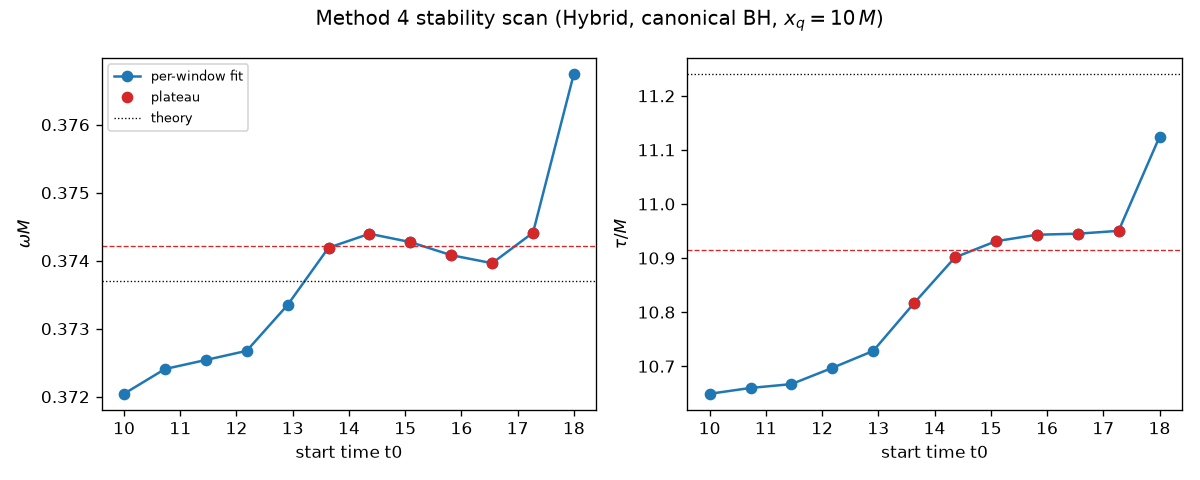
\includegraphics[width=0.80\textwidth]{../outputs/hybrid/fno_sw_gate_s1em3/figs/hybrid_plateau_m4_xq10.png}
\caption{M4 1-D plateau scan on the hybrid prediction at the
canonical BH and $\xq = 10\,M$. Per-window two-mode NLS fits
(blue circles) on $t_{0} \in [10, 18]\,M$ at fixed
$\tend = 50\,M$; the red circles mark the contiguous plateau
block of $6$ start times on $t_{0} \in [13.6, 17.3]\,M$ used to
form the canonical M4 estimate. Black
dotted lines mark the Leaver reference values $\omega = 0.3737$
and $\tau = 11.241\,M$.}
\label{fig:hyb-plateau-m4}
\end{figure}

\paragraph{Training history.} A single Adam phase reduces the
validation MSE on the gated Richardson residual from
$3.6\times 10^{-4}$ to $1.8\times 10^{-6}$ over $100$ epochs,
with train and validation tracking together
(Fig.~\ref{fig:hyb-loss}).

\begin{figure}[!htbp]
\centering
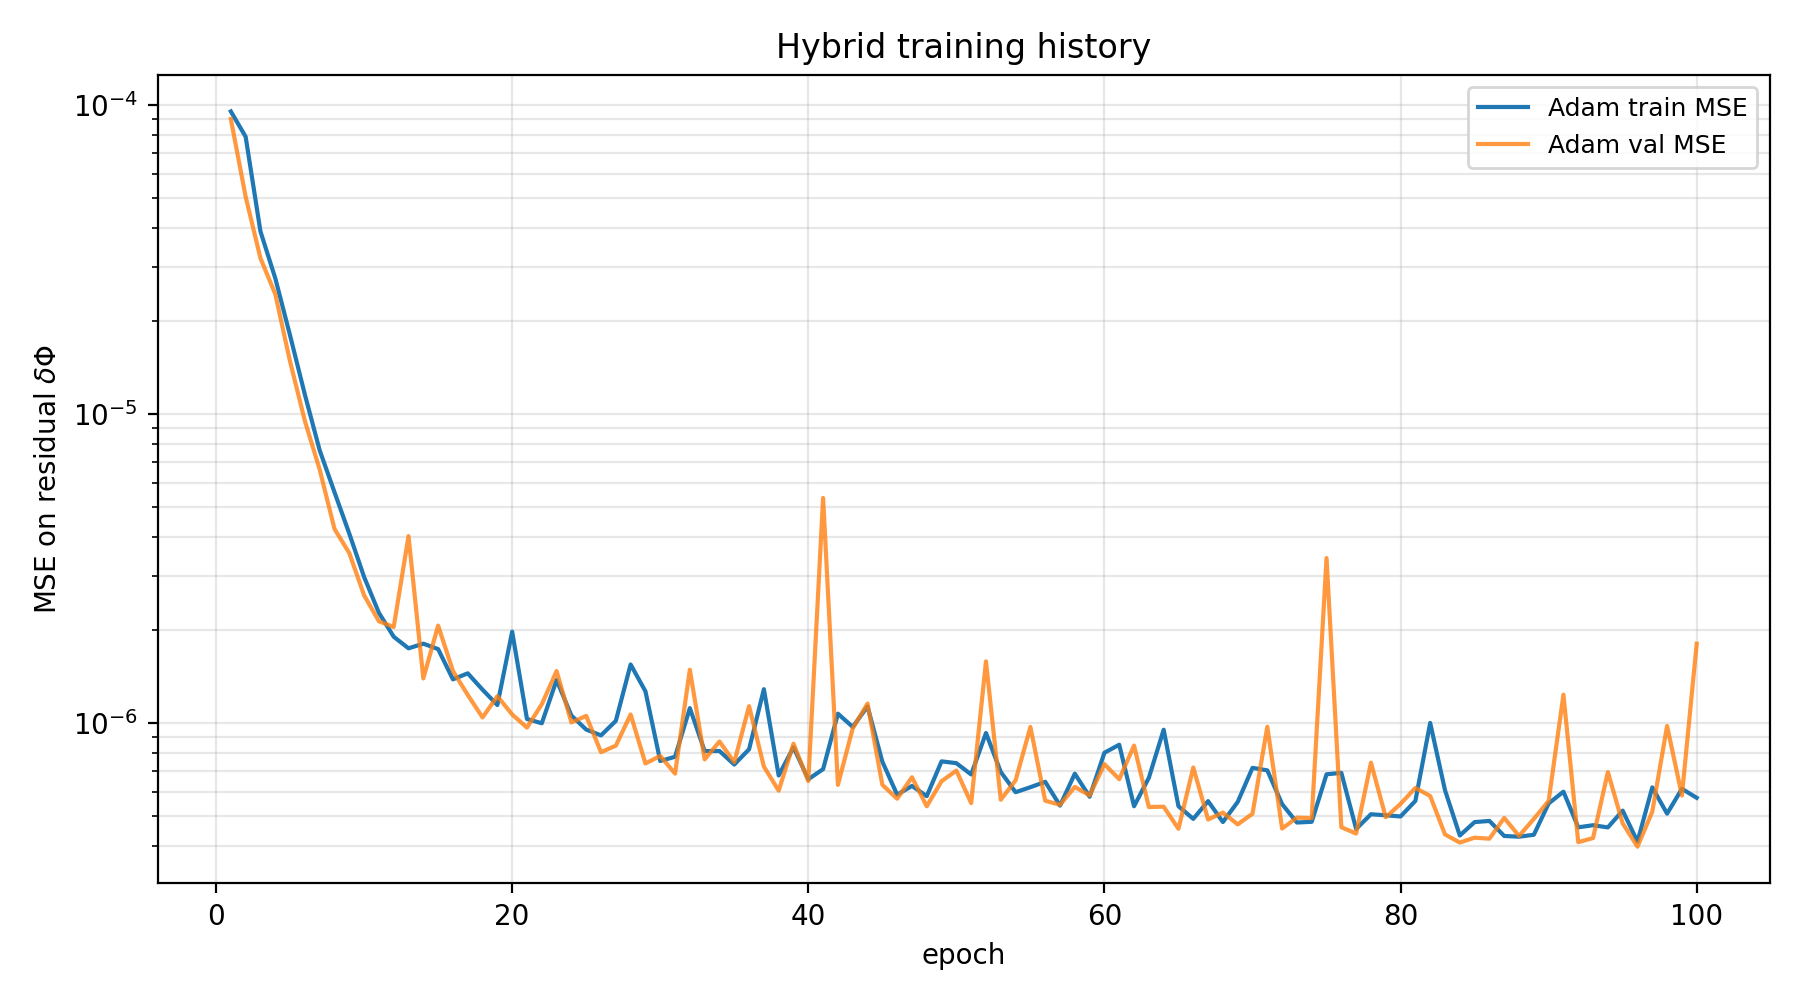
\includegraphics[width=0.85\textwidth]{../outputs/hybrid/fno_sw_gate_s1em3/figs/hybrid_loss.png}
\caption{Hybrid surrogate training history: per-epoch train and
validation MSE on the gated Richardson residual over $100$ Adam
epochs.}
\label{fig:hyb-loss}
\end{figure}

\FloatBarrier

% ==============================================================
\subsection{Generalisation to Kerr}
\label{sec:res-kerr}

The final experiment asks whether the hybrid construction is
tied to the Schwarzschild geometry. We retrain the surrogate on
a $128$-black-hole test set drawn from a Sobol sequence in
dimensionless spin $a/M \in [0, 0.95]$, evolving the
hyperboloidal Teukolsky field of Sec.~\ref{sec:teukolsky-problem} and
targeting the fundamental $(\ell, m, n) = (4, 2, 0)$ mode.
Table~\ref{tab:kerr-summary} collects the field and frequency
accuracy by spin bin.

\paragraph{Field.} Across the test set the coarse prior carries
a median relative $L^{2}$ field error of $59.5\%$: at low
resolution the hyperboloidal wavefront is badly
under-resolved. The hybrid reduces this to $0.78\%$, a factor
of $77$, and the error stays nearly flat across spin --- from
$0.70\%$ at low spin to $1.08\%$ near extremality
(Table~\ref{tab:kerr-summary}) --- so a single amortised
operator absorbs almost the entire spin dependence of the
field. The label-free Richardson target itself sits at
$0.008\%$, confirming that the FNO, not the reference, sets the
floor. Figure~\ref{fig:kerr-ringdown} overlays the
reconstructed ringdown at $\scri$ against the fine reference
for a representative $a/M = 0.7$ black hole, and
Fig.~\ref{fig:kerr-pointwise} shows the coarse solve's error
concentrated in the high-amplitude burst, which the residual
correction removes.

\paragraph{Frequency.} The amortisation is clearest at high
spin, where the coarse prior degrades fastest. For
$a/M \ge 0.8$ ($20$ black holes) the best-of-suite prior
frequency error is $4.71\%$, which the hybrid cuts to $0.38\%$
--- a $12\times$ improvement --- approaching the fine-solve
floor of $0.02\%$ (Table~\ref{tab:kerr-summary},
Fig.~\ref{fig:kerr-vs-spin}). Pooled over all spins the median
frequency error falls from $0.59\%$ to $0.33\%$, with the fine
solve at $0.05\%$. The correction is largest exactly where it
is needed: at moderate spin the prior is already sub-percent
and the hybrid tracks it, whereas near extremality --- where
the near-horizon oscillation of Eq.~\eqref{eq:kerr-rescale} is
strongest and the coarse grid fails --- the hybrid recovers
more than an order of magnitude.

\paragraph{Damping time.} The damping time is the harder
channel (Fig.~\ref{fig:kerr-vs-spin}c), exactly as for the
Zerilli surrogate (Sec.~\ref{sec:res-hyb}). Pooled over spin the
hybrid $\tau$
error ($1.52\%$) exceeds that of the coarse prior ($0.52\%$),
while the fine solve ($0.27\%$) shows that the residual
correction --- tuned to the field and its leading oscillation
--- does not consistently sharpen the exponential envelope.
This is the same trade-off seen for Schwarzschild: the operator
restores the phase and amplitude of the field far better than
its slowly varying decay rate, so $\tau$ remains a fine-solve
quantity and the surrogate is a frequency-and-field
accelerator rather than a damping-time estimator.

\paragraph{Verdict.} Taken together, the Kerr experiment shows
that the hybrid concept is geometry-agnostic. The same
coarse-plus-residual construction, retrained without a single
fine-grid field in its loss, transfers from a static
Schwarzschild wave equation to a rotating, complex,
hyperboloidal Teukolsky field and still delivers an
order-of-magnitude field improvement and sub-percent
frequencies across the astrophysical spin range --- a
generalisation that a per-black-hole PINN, retrained from
scratch for every spin, does not provide.

\begin{table}[!htbp]
\centering
\caption{Kerr hybrid surrogate accuracy by spin bin over the
$128$-black-hole test set: bin medians, with the final row the
population median. Field errors are relative $L^{2}$ against the
fine solve, for the coarse prior, the hybrid, and the label-free
Richardson target. Frequency ($|\delta\omega|/\omega$) and
damping-time ($|\delta\tau|/\tau$) errors are the best-of-suite
values for the $(4,2,0)$ mode, with the fine-solve error shown
for reference. The estimator winning most often for the hybrid
is noted below the table
(M3 $=$ selective ESPRIT, cES $=$ complex ESPRIT,
c$\Phi$ $=$ complex-phase fit; Sec.~\ref{sec:teukolsky-problem}).}
\label{tab:kerr-summary}
\footnotesize
\setlength{\tabcolsep}{4pt}
\begin{tabular}{lr rrr rrr rrr}
\toprule
 & & \multicolumn{3}{c}{Field rel-$L^{2}$ (\%)}
   & \multicolumn{3}{c}{$M\omega$ err.\ (\%)}
   & \multicolumn{3}{c}{$\tau/M$ err.\ (\%)} \\
\cmidrule(lr){3-5}\cmidrule(lr){6-8}\cmidrule(lr){9-11}
$a/M$ & $n$ & prior & hybrid & Rich.
      & prior & hybrid & fine
      & prior & hybrid & fine \\
\midrule
$[0.0,0.3]$  & $41$ & $51.2$ & $0.70$ & $0.004$ & $0.63$ & $0.53$ & $0.06$ & $0.56$ & $1.79$ & $0.46$ \\
$[0.3,0.6]$  & $40$ & $59.1$ & $0.70$ & $0.006$ & $0.44$ & $0.27$ & $0.08$ & $0.29$ & $1.67$ & $0.42$ \\
$[0.6,0.8]$  & $27$ & $65.7$ & $0.86$ & $0.013$ & $0.39$ & $0.23$ & $0.04$ & $0.32$ & $1.22$ & $0.16$ \\
$[0.8,0.95]$ & $20$ & $73.6$ & $1.08$ & $0.063$ & $4.71$ & $0.38$ & $0.02$ & $1.43$ & $2.19$ & $0.02$ \\
\midrule
All (median) & $128$ & $59.5$ & $0.78$ & $0.008$ & $0.59$ & $0.33$ & $0.05$ & $0.52$ & $1.52$ & $0.27$ \\
\bottomrule
\end{tabular}

\smallskip
{\footnotesize\raggedright Dominant hybrid estimator by
ascending spin bin --- $M\omega$: cES, M3, M3, M3 (M3 overall);
$\tau/M$: cES, cES, M3, c$\Phi$ (cES overall).\par}
\end{table}

\begin{figure}[!htbp]
\centering
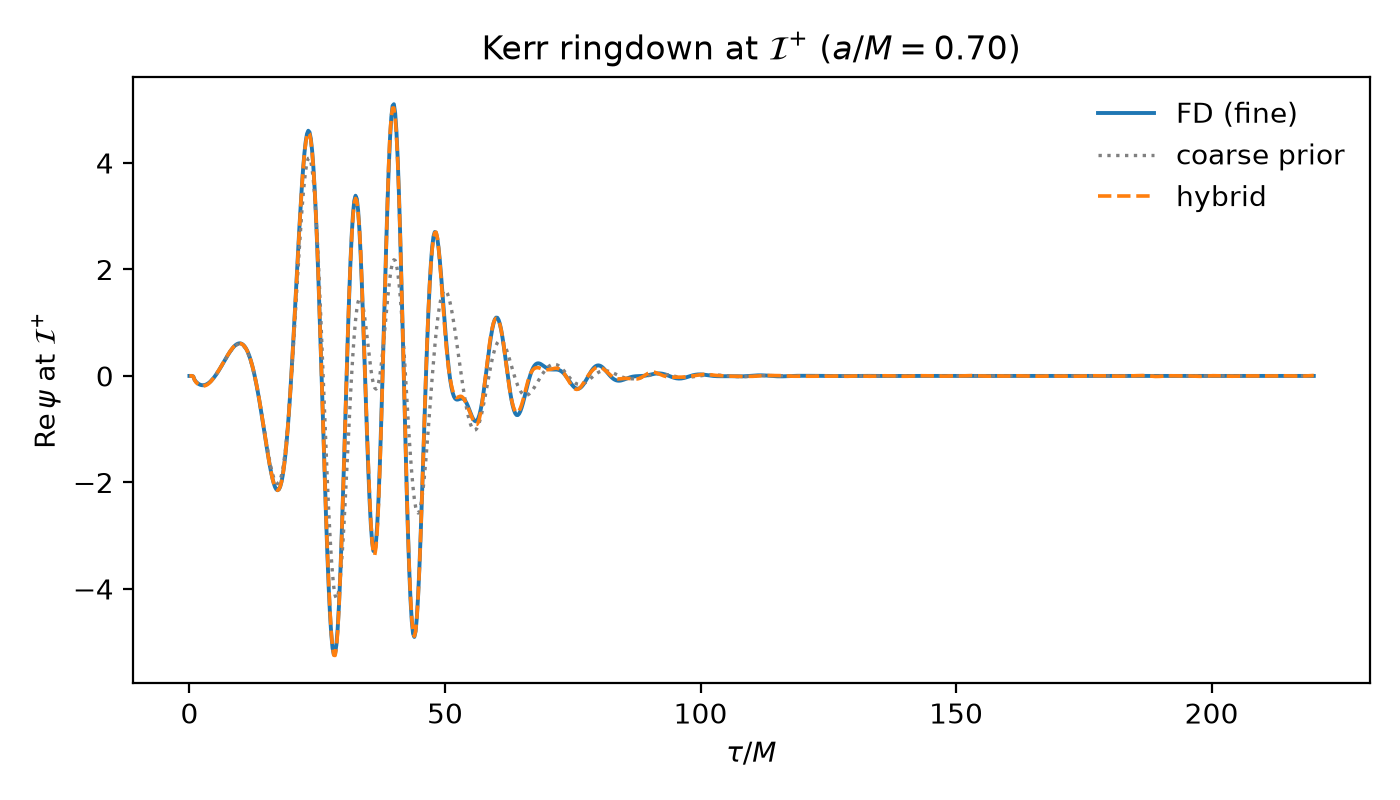
\includegraphics[width=0.82\textwidth]{../outputs/kerr/figs/hybrid_ringdown_scri.png}
\caption{Kerr ringdown at null infinity $\scri$ for a
representative $a/M = 0.7$ black hole. The hybrid (orange,
dashed) overlays the fine reference (blue, solid), whereas the
coarse prior (grey, dotted) departs from it in amplitude and
phase through the peak of the burst.}
\label{fig:kerr-ringdown}
\end{figure}

\begin{figure}[!htbp]
\centering
\begin{subfigure}[t]{0.49\textwidth}
\centering
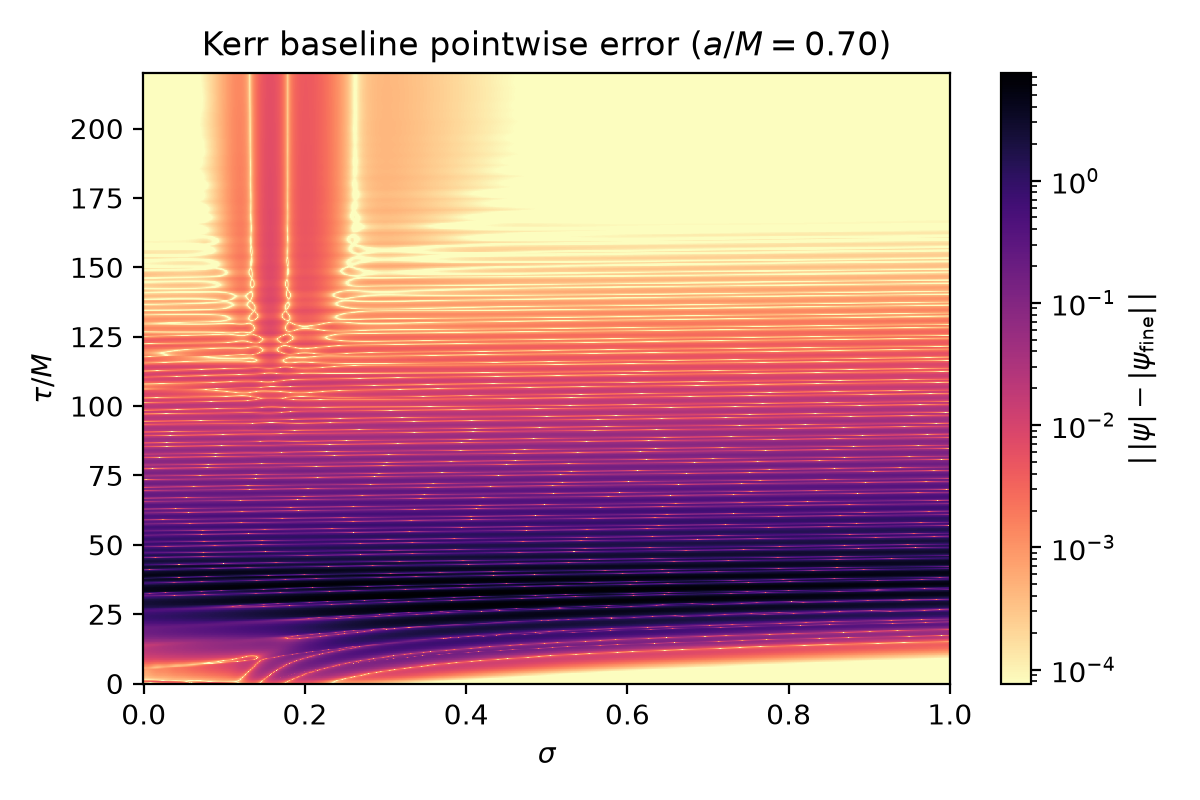
\includegraphics[width=\textwidth]{../outputs/kerr/figs/hybrid_pointwise_error_baseline.png}
\subcaption{Coarse prior.}
\end{subfigure}
\hfill
\begin{subfigure}[t]{0.49\textwidth}
\centering
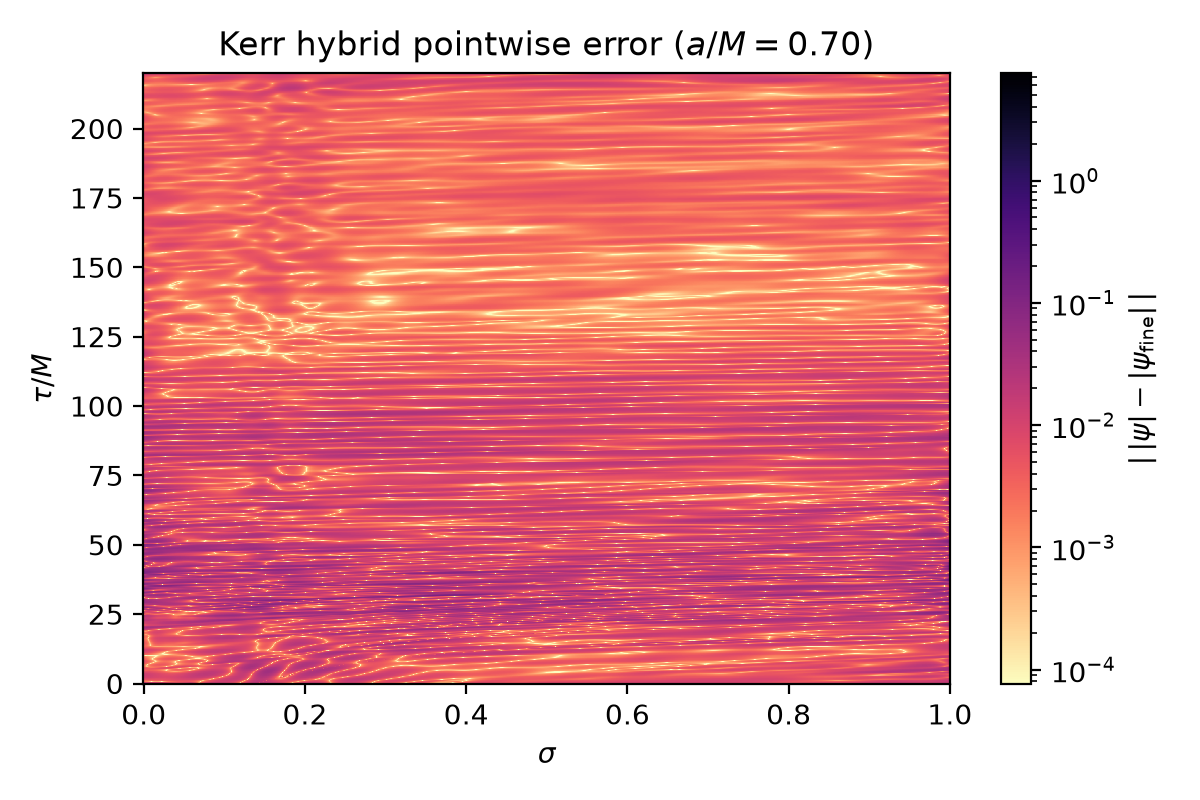
\includegraphics[width=\textwidth]{../outputs/kerr/figs/hybrid_pointwise_error_hybrid.png}
\subcaption{Hybrid.}
\end{subfigure}
\caption{Pointwise field error over the compactified domain
$(\sigma, \tau)$, both panels on the same logarithmic colour
scale. The coarse prior (a) concentrates its error in the
high-amplitude burst phase (early $\tau$); the residual FNO (b)
removes that burst-phase structure, leaving a much lower
residual across the domain.}
\label{fig:kerr-pointwise}
\end{figure}

\begin{figure}[!htbp]
\centering
\begin{subfigure}[t]{0.49\textwidth}
\centering
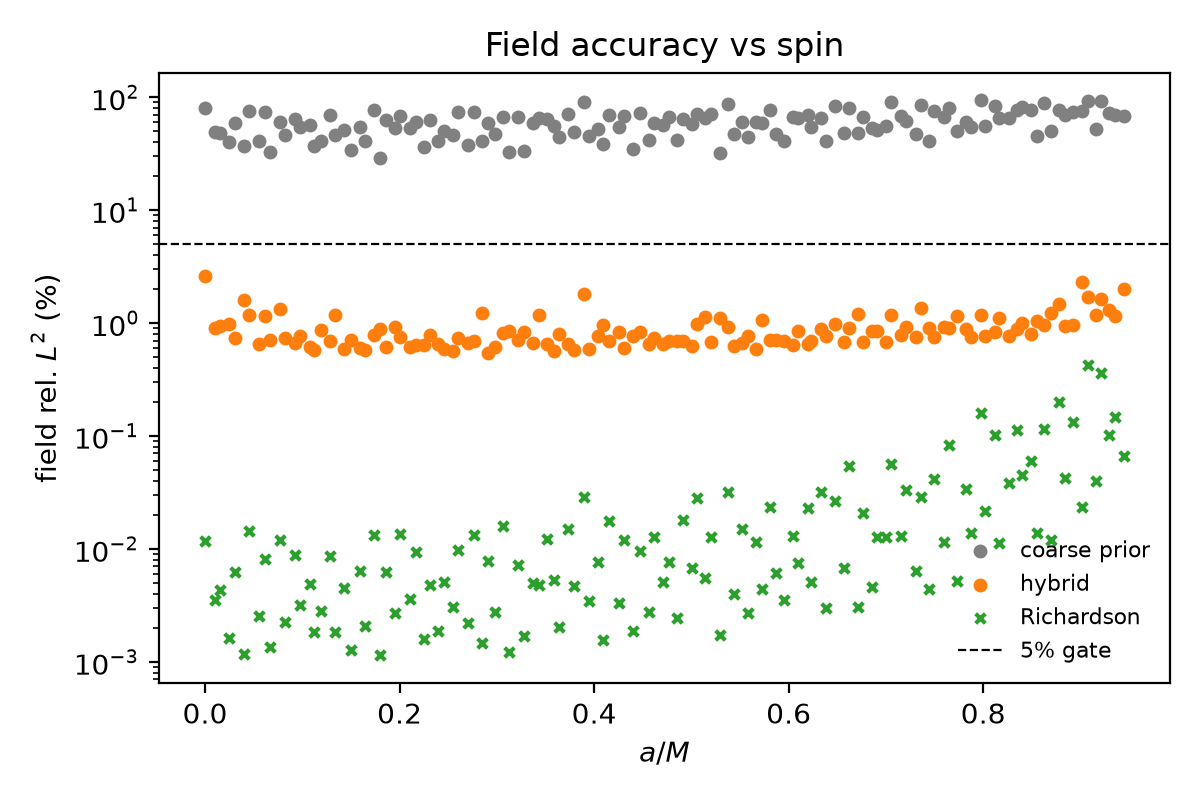
\includegraphics[width=\textwidth]{../outputs/kerr/figs/hybrid_field_vs_spin.png}
\subcaption{Field error.}
\end{subfigure}
\hfill
\begin{subfigure}[t]{0.49\textwidth}
\centering
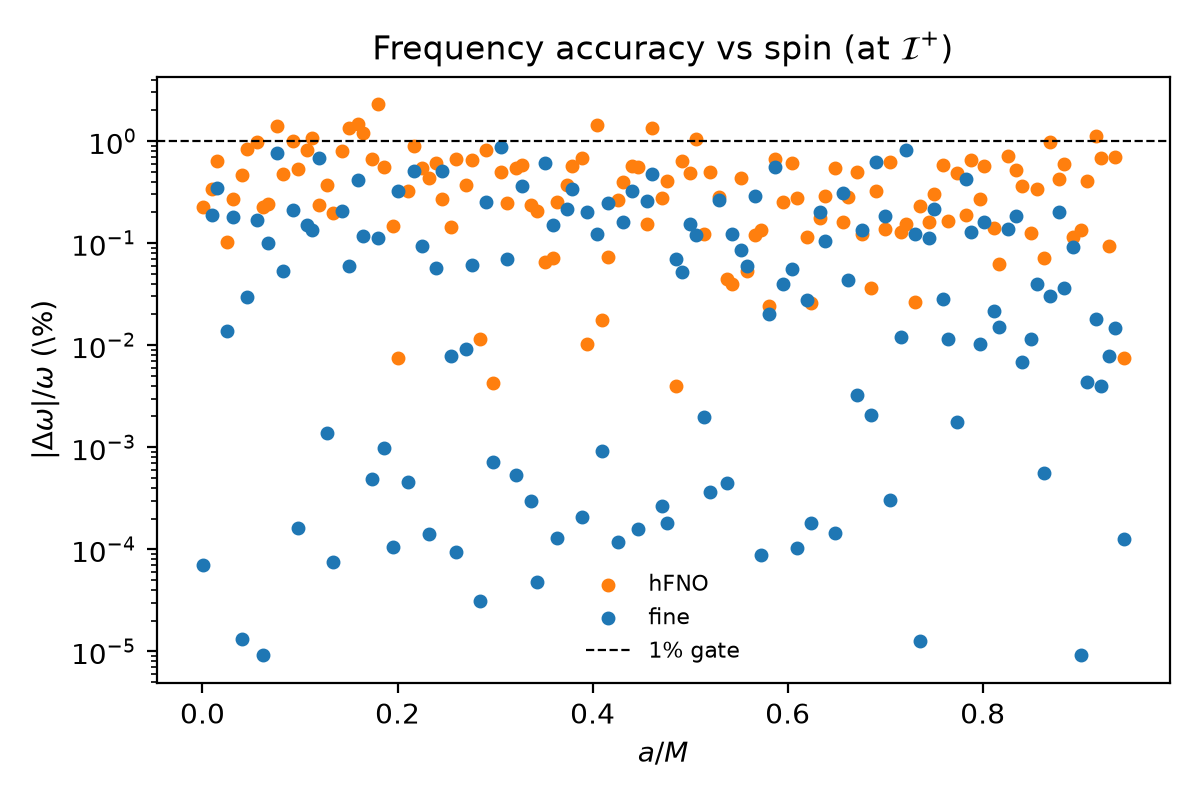
\includegraphics[width=\textwidth]{../outputs/kerr/figs/hybrid_qnm_vs_spin.png}
\subcaption{Frequency error.}
\end{subfigure}

\vspace{0.6em}
\begin{subfigure}[t]{0.49\textwidth}
\centering
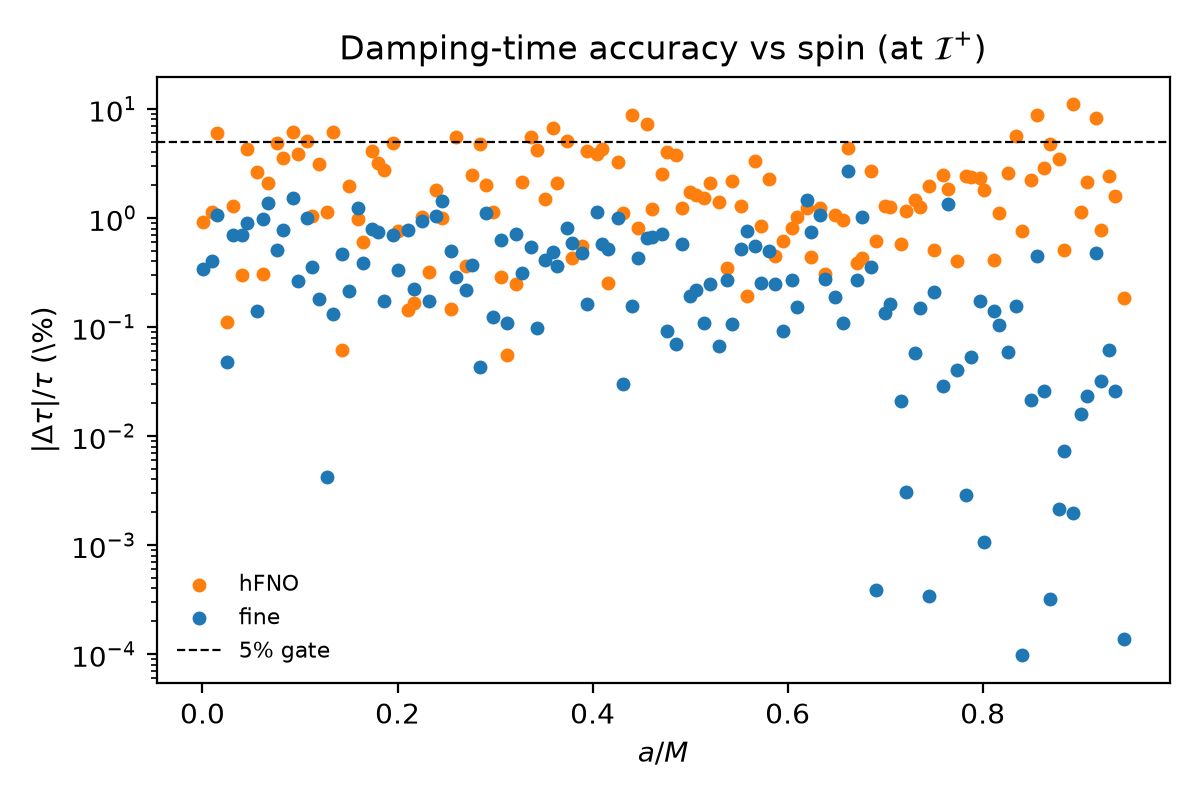
\includegraphics[width=\textwidth]{../outputs/kerr/figs/hybrid_tau_vs_spin.png}
\subcaption{Damping-time error.}
\end{subfigure}
\caption{Best-of-suite accuracy versus spin (coarse prior grey,
hybrid orange; fine reference blue in (b) and (c), label-free
Richardson target green in (a)). (a)~The hybrid field error is
flat across $a/M$ while the coarse prior grows towards
extremality. (b)~The prior frequency error spikes for
$a/M \gtrsim 0.8$, where the hybrid recovers more than an order
of magnitude and approaches the fine-solve floor. (c)~The
damping time is the exception: the hybrid does not improve on
the prior and stays well above the fine floor, as discussed in
the text.}
\label{fig:kerr-vs-spin}
\end{figure}

\FloatBarrier


% =====================================================================
% =============================================================
% Section 5: Discussion
% =============================================================
\section{Discussion}\label{sec:discussion}

\paragraph{Schwarzschild and Kerr field errors.}
The hFNO is our principal contribution, combining a
reduced-resolution numerical prior with correction operators trained
separately on the Schwarzschild and Kerr parameter sets. The coarse
finite-difference solve enforces the propagation, scattering and
boundary treatment of each perturbation equation, while the neural
operator corrects the discretisation error introduced by
under-resolution. Neither hFNO requires per-configuration
neural-network optimisation.

\paragraph{Evidence from Schwarzschild and Kerr.}
Across the Schwarzschild configurations, the hFNO reduces the mean
relative $L^2$ error from $13.39\%$ to $1.85\%$ and the field MSE by
a factor of $46$. Figure~\ref{fig:hyb-grad} shows a correlation
$r=0.921$ between $d_{\mathrm{idx}}$ and numerical-prior error, which
is concentrated near propagating wavefronts. For
Kerr, the median relative $L^2$ error falls from $59.5\%$ to $0.78\%$,
and the high-spin median frequency error is $0.38\%$. The
Richardson-extrapolated field reaches $0.008\%$, showing that the
remaining discrepancy arises primarily from the learned correction
rather than the target construction.

\paragraph{QNM extraction.}
Across the Schwarzschild configurations, M4 gives a median frequency
error of $0.152\%$. For Kerr, the retrospective Leaver-closest
selection gives median errors of $0.33\%$ in
frequency and $1.52\%$ in damping time, compared with $0.05\%$
and $0.27\%$ from the fine reference fields. Appendix~\ref{app:kerr-extractors}
shows the estimator dependence and distinguishes retrospective
selection from the pre-specified target-mode ensemble. The larger damping-time
error is consistent with training being dominated by the
high-amplitude burst and wavefronts, whereas damping depends on the
low-amplitude late-time envelope. The hFNO loss minimises full-field
mean-squared error and does not directly optimise QNM frequency or
damping time.

\paragraph{Scope and limitations.}
The test configurations lie within the parameter ranges used for
training, use one perturbative harmonic in each geometry and require
separate training for the Schwarzschild and Kerr formulations. The
fixed-grid Fourier representation has not been tested under
changes of domain, resolution or boundary treatment. The
gradient gate reduces the global Schwarzschild mean-squared error,
while the pointwise maps show smaller gains where the numerical prior
is already accurate.
Richardson extrapolation also relies on the two coarse
discretisations lying within the expected convergence regime.
The field results apply to the $\ell=2$ Zerilli and
$(\ell,m)=(4,2)$ Teukolsky sectors studied here; the reported QNM
errors concern their fundamental modes.

\paragraph{Future directions.}
The late-time errors in Figs.~\ref{fig:kerr-ringdown}
and~\ref{fig:kerr-pointwise} motivate late-time-sensitive objectives,
temporal decomposition or solver-in-the-loop training
\citep{Um2020solverloop,Wang2023longtime,McCabe2023stability}.
Initial data designed to excite stronger overtone content and
additional harmonics would test a broader range of ringdown signals.
End-to-end timing should measure the wall-clock reduction and training
break-even point.

Observer waveforms generated by the Schwarzschild and Kerr hFNOs
could also be incorporated into Bayesian inference. Reduced bases and
reduced-order quadratures
accelerate repeated gravitational-wave likelihood evaluations while
controlling the approximation error
\citep{Canizares2013roq,Canizares2015roq}. Constructing a reduced
basis from the hFNO waveforms would measure likelihood-evaluation cost
and propagate detector noise, hFNO field error and fit-window
dependence into parameter estimates.


% =====================================================================
\section{Conclusion}\label{sec:conclusion}

We benchmarked a faithful reproduction of
\citet{Patel2024pinn}, an enhanced forward PINN and a hybrid
Fourier neural operator on time-domain black-hole
perturbations, using post-hoc QNM estimates as diagnostics of
the computed fields. The faithful reproduction yields field
errors an order of magnitude below the values reported for both
Schwarzschild $\ell=2$ potentials. Residual-greedy sampling and
an extended L-BFGS stage reduce the Zerilli field error to
$0.58\%$, with best-of-suite fundamental-mode errors of
$0.029\%$ in frequency and $1.99\%$ in damping time relative
to the Leaver values.

The principal result is the hFNO, which learns a correction to
a coarse numerical trajectory from a Richardson estimate formed
without fine-grid training fields. Across the $100$-configuration
Schwarzschild test population, it reduces the mean field error
from $13.39\%$ to $1.85\%$ and the field MSE by a factor of
$46$, while recovering the fundamental frequency to $0.152\%$.
After adaptation to the complex hyperboloidal Teukolsky field
and separate retraining, the Kerr hFNO reduces the
population-median field error from $59.5\%$ to $0.78\%$. In the
high-spin bin, the frequency error decreases from $4.71\%$ to
$0.38\%$.

These results demonstrate that the coarse-prior-plus-residual
design is effective across the two tested perturbation
formulations and their sampled parameter ranges. The Kerr
damping-time error nevertheless increases from $0.52\%$ to
$1.52\%$, identifying the low-amplitude late-time field as the
main unresolved limitation. Late-time-sensitive training and
an end-to-end runtime comparison are therefore the immediate
tests required to establish the method's practical value.

% =====================================================================
\section*{Code availability}

The accompanying repository contains the configurations, run
scripts, numerical solvers, extraction methods and analysis
scripts used in this report. Large trained-model and dataset
artifacts that cannot be included directly are identified in the
repository documentation.

% =====================================================================
\appendix
\section{Finite-difference reference solver}\label{app:fd}

Eq.~\eqref{eq:zerilli} is integrated in first-order-in-time
form ($\Pi \equiv \partial_t\Phi$) on the grid of
Sec.~\ref{sec:fwd-problem}. Table~\ref{tab:fd-scheme} summarises
the scheme; the full stencil-level specification is in the
repository documentation.

\begin{table}[!htbp]
\centering
\caption{Finite-difference reference solver (grid and step sizes
in Table~\ref{tab:fwd-hyper}).}
\label{tab:fd-scheme}
\small
\begin{tabular}{ll}
\hline
Property & Value \\
\hline
Formulation        & first-order in time, $\Pi \equiv \partial_t\Phi$ \\
Interior stencil   & three-point centred (2nd order) \\
Boundary closures  & second-order one-sided \\
Time integration   & fourth-order Runge--Kutta (method of lines) \\
Boundary condition & algebraic Sommerfeld (outgoing) \\
Courant factor     & $\nu = 0.5$ (stable) \\
Earliest reflection & $t \ge 108\,M$, outside $t_{\max} = 50\,M$ \\
\hline
\end{tabular}
\end{table}

% =====================================================================
% =====================================================================
\section{Supplementary scans and diagnostics}
\label{app:supp}

This appendix collects the parameter scans, ablations and
diagnostics that justify the configuration choices reported in
Sec.~\ref{sec:results}.

\subsection{Inverse PINN: template diagnostics}
\label{app:supp-inv}

Tables~\ref{tab:inv-learned} and~\ref{tab:tau-degeneracy} list
the learned template scalars for the six inverse variants and
compare $\tau_{\mathrm{learned}}$ with the post-hoc M2
wide-window fit: the strongly template-weighted variants (A, D,
E) drift $1.2$--$1.9\,M$ below the post-hoc value along the
$A_{\mathrm{ring}}$--$\tau$ degeneracy of
Eq.~\eqref{eq:loss-ring} while the field retains the physical
decay rate --- the quantitative basis for the reporting
convention of Sec.~\ref{sec:reporting}.

\begin{table}[!htbp]
\centering
\caption{Inverse PINN learned template parameters at the end of
training for each
variant. These are the values of the learnable scalars
$(\omega,\tau,A_{\mathrm{ring}},\phi)$ inside the ringdown loss of
Eq.~\eqref{eq:loss-ring} after $10{,}000$ Adam plus $15{,}000$
L-BFGS iterations. They are reported as a diagnostic and are not
the primary QNM estimates of Table~\ref{tab:inv-summary}; the
reason is given in the
$A_{\mathrm{ring}}$--$\tau$ paragraph below.}
\label{tab:inv-learned}
\small
\begin{tabular}{@{}lcccc@{}}
\toprule
Variant & $\omega_{\mathrm{learned}}$ & $\tau_{\mathrm{learned}}/M$ &
        $A_{\mathrm{ring}}$ & $\phi$ \\
\midrule
baseline   & $0.3820$ & $11.89$ & $1.92$ & $-0.99$ \\
A          & $0.3704$ & $10.10$ & $2.59$ & $-0.72$ \\
B          & $0.4050$ & $8.62$  & $2.97$ & $-1.38$ \\
C          & $0.3822$ & $11.84$ & $1.92$ & $-0.99$ \\
D          & $0.3748$ & $9.48$  & $2.93$ & $-0.85$ \\
E (mode 0) & $0.3496$ & $9.22$  & $2.52$ & $+0.31$ \\
E (mode 1) & $0.3810$ & $7.38$  & $3.24$ & $-1.90$ \\
\bottomrule
\end{tabular}
\end{table}

\begin{table}[!htbp]
\centering
\caption{$A_{\mathrm{ring}}$--$\tau$ degeneracy diagnostic. The
training-time learned $\tau_{\mathrm{learned}}$ is the value of the
learnable scalar at the end of training. The post-hoc M2 wide-window
$\tau_{\mathrm{M2}}^{\mathrm{wide}}$ is the M2 fit to
$\Phi_\theta(\xq,t)$ over $[10,50]\,M$. Truth is
$\tau_0/M = 11.241$ \citep{Leaver1985}. ``Bias gap'' is
$|\tau_{\mathrm{learned}} - \tau_{\mathrm{M2}}^{\mathrm{wide}}|/M$.
For variant E, $\tau_{\mathrm{learned}}$ refers to the fundamental
template mode (mode 0).}
\label{tab:tau-degeneracy}
\small
\begin{tabular}{@{}lccc@{}}
\toprule
Variant & $\tau_{\mathrm{learned}}/M$ & $\tau_{\mathrm{M2}}^{\mathrm{wide}}/M$ & Bias gap \\
\midrule
baseline & $11.89$ & $11.83$ & $0.06$ \\
A        & $10.10$ & $11.29$ & $1.19$ \\
B        & $8.62$  & $8.63$  & $0.01$ \\
C        & $11.84$ & $11.82$ & $0.02$ \\
D        & $9.48$  & $11.06$ & $1.58$ \\
E        & $9.22$  & $11.10$ & $1.88$ \\
\bottomrule
\end{tabular}
\end{table}

\subsection{Hybrid: gradient-gate diagnostics}
\label{app:supp-gate}

Figure~\ref{fig:hyb-grad} shows the per-cell scatter of
coarse-prior error against prior gradient magnitude on the
canonical BH (log--log Pearson $r = 0.917$), the empirical
basis of the gradient gate, and
Table~\ref{tab:hyb-gate-decile} the decile stratification: the
gated correction reduces the mean error by $14.1\times$ in the
top gradient decile, declining monotonically to $2.6\times$ in
the sixth, with the sub-median cells left at the prior floor.
The gate scale itself is fixed label-free in
Appendix~\ref{app:gate-scale}.

\begin{figure}[!htbp]
\centering
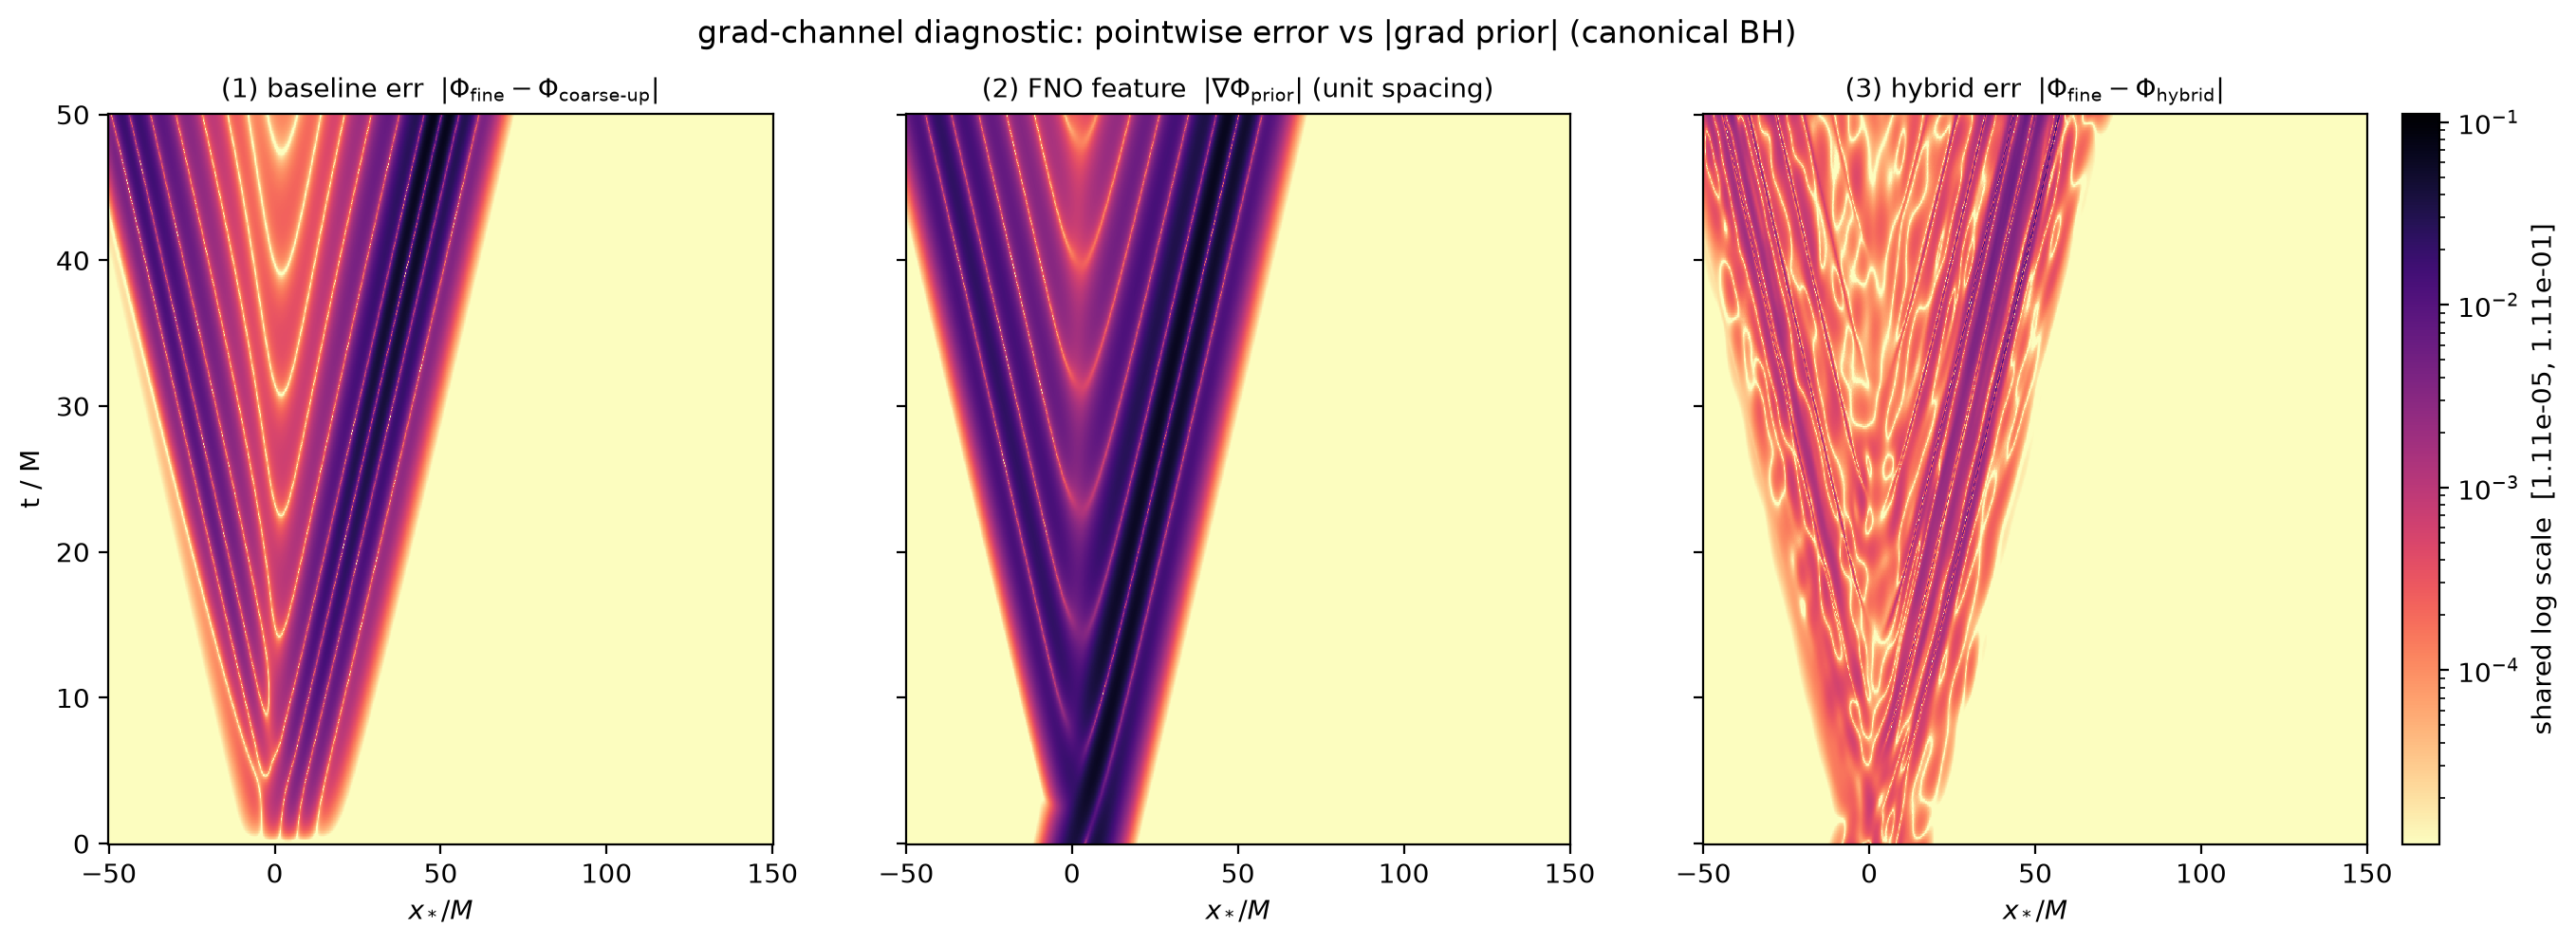
\includegraphics[width=0.82\textwidth]{../outputs/hybrid/fno_sw_gate_s1em3/figs/grad_vs_error.png}
\caption{Coarse-prior error versus prior gradient on the
canonical BH, the diagnostic motivating the gradient gate.
Each point is one $(x,t)$ cell; the horizontal axis is the
prior gradient magnitude $|\nabla\mathcal{U}\Phi^{\mathrm{c}}|$
and the vertical axis the coarse-up baseline error
$|\Phi^{\mathrm{f}} - \mathcal{U}\Phi^{\mathrm{c}}|$, both on
log scales. The log--log Pearson correlation is $r = 0.917$:
the prior error is large precisely on the high-gradient
wavefronts and small in the low-gradient interior and causal
exterior, so the gate $g$ (Eq.~\eqref{eq:hyb-gate}) routes the
network correction to the cells that need it.}
\label{fig:hyb-grad}
\end{figure}

\begin{table}[!htbp]
\centering
\caption{Hybrid error reduction stratified by coarse-prior
gradient on the canonical BH. Cells are sorted into deciles of
$|\nabla\mathcal{U}\Phi^{\mathrm{c}}|$; for the top four
deciles (the wavefront-bearing cells) the table lists the
decile-mean gradient, the mean coarse-up baseline error, the
mean hybrid error, and their ratio. Below the median the prior
gradient is $\lesssim 10^{-12}$ (smooth interior and causal
exterior) and both errors are at the field floor.}
\label{tab:hyb-gate-decile}
\small
\setlength{\tabcolsep}{6pt}
\begin{tabular}{@{}lcccc@{}}
\toprule
Gradient decile & $\overline{|\nabla\mathcal{U}\Phi^{\mathrm{c}}|}$
 & baseline err & hybrid err & ratio \\
\midrule
90--100\% (wavefronts) & $3.15\times 10^{-2}$ & $1.30\times 10^{-2}$ & $9.22\times 10^{-4}$ & $14.1$ \\
80--90\%               & $1.01\times 10^{-2}$ & $4.37\times 10^{-3}$ & $4.42\times 10^{-4}$ & $9.9$  \\
70--80\%               & $3.56\times 10^{-3}$ & $2.21\times 10^{-3}$ & $2.58\times 10^{-4}$ & $8.6$  \\
60--70\%               & $4.37\times 10^{-4}$ & $6.81\times 10^{-4}$ & $2.60\times 10^{-4}$ & $2.6$  \\
\bottomrule
\end{tabular}
\end{table}

\subsection{Hybrid M5 plateau diagnostic}
\label{app:supp-m5}

Figure~\ref{fig:hyb-plateau-m5}
shows the M5 2-D plateau scan for the hybrid canonical
extraction; it confirms the main-text M4 value
(Table~\ref{tab:hyb-canonical}).

\begin{figure}[!htbp]
\centering
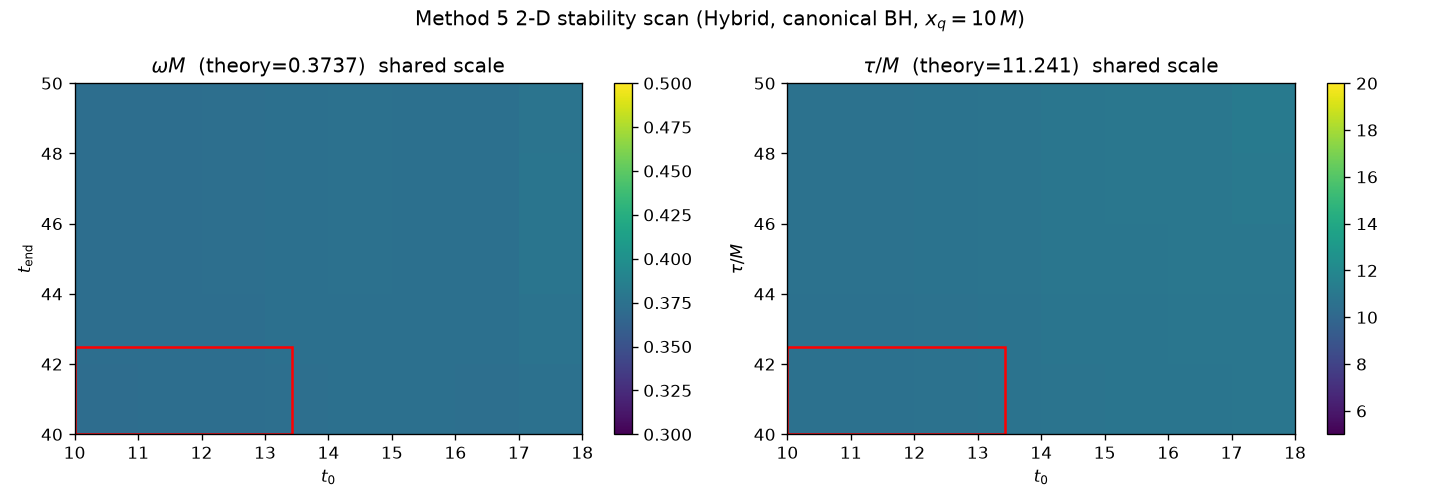
\includegraphics[width=0.95\textwidth]{../outputs/hybrid/fno_sw_gate_s1em3/figs/hybrid_plateau_m5_xq10.png}
\caption{M5 2-D plateau scan on the hybrid prediction at the
canonical BH and $\xq = 10\,M$. Heatmaps of the fitted
$\omega$ (left) and $\tau$ (right) over an $8 \times 5$ grid in
$(t_{0}, \tend)$ with $t_{0} \in [10, 18]\,M$ and
$\tend \in [40, 50]\,M$, on the shared colour scales
$\omega \in [0.30, 0.50]$ and $\tau \in [5, 20]\,M$. The red
rectangle marks the identified plateau block
($t_{0} \in [10.0, 13.4]\,M$,
$\tend \in [40.0, 42.5]\,M$). White cells are NLS fits that
failed to converge.}
\label{fig:hyb-plateau-m5}
\end{figure}


% =====================================================================
\section{Hyperparameter tables}\label{app:hyper}

This appendix collects the full hyperparameter list for the
forward PINN of Sec.~\ref{sec:fwd-pinn}.

\begin{table}[!htbp]
\centering
\caption{Architecture and training hyperparameters for the
forward PINN of Sec.~\ref{sec:fwd-pinn}.}
\label{tab:fwd-hyper}
\small
\begin{tabular}{lll}
\hline
Block & Parameter & Value \\
\hline
Domain
  & $x \in [x_{\min}, x_{\max}]\,M$ & $[-50,\,150]$ \\
  & $t \in [t_{\min}, t_{\max}]\,M$ & $[0,\,50]$ \\
Initial data
  & amplitude $A_0$, centre $x_0/M$, width $\sigma_0/M$
  & $1.0,\;4.0,\;5.0$ \\
  & velocity profile & outgoing \\
FD reference
  & $\Delta x/M,\;\Delta t/M,\;$scheme
  & $0.2,\;0.1,\;$RK4--MoL \\
Network
  & hidden layers (widths)            & $[80,\,40,\,20,\,10]$ \\
  & activation, output transform      & tanh, $A\tanh(\cdot)\,\mathrm{NN}$ \\
  & dtype, seed                       & float64, $1234$ \\
Collocation
  & $N_r,\;N_i,\;N_b$ & $32\,000,\;800,\;400$ \\
Loss weights
  & $\lambda = (\lambda_r,\lambda_{r_x},\lambda_{r_t},
              \lambda_{\mathrm{ic}},\lambda_{\mathrm{iv}},
              \lambda_{b_L},\lambda_{b_R})$
  & $(100,100,100,1,100,1,1)$ \\
Adam
  & learning rate, iterations        & $10^{-3},\;10\,000$ \\
L-BFGS
  & iterations                       & $30\,000$ \\
Adaptive sampling
  & method, period, candidates       & greedy, $1000$, $100\,000$ \\
  & greedy fraction $f$              & $0.3$ \\
Observer
  & $x_{\mathrm{obs}}/M$             & $10.0$ \\
QNM window
  & $[t_{0},\tend]/M$ & $[10,\,50]$ \\
\hline
\end{tabular}
\end{table}

\section{Principled choice of the gradient-gate scale}\label{app:gate-scale}

The gate scale $s$ is the only free gate parameter. Sweeping it
label-free from the single trained model
(Table~\ref{tab:gate-scale-sweep}), the global RMSD varies by
$<2\%$ across a flat basin that contains the deployed
$s = 10^{-3}$. That value equals the $68$th percentile of the
prior-gradient distribution, giving the label-free rule
$s \simeq Q_{0.68}(|\nabla\,\mathcal{U}\Phi^{\mathrm{c}}|)$, a
function of the coarse prior alone. The re-gating identity is
derived in the repository documentation.

\begin{table}[!htbp]
\centering
\caption{Field error of the canonical-BH hybrid as a function of
the gate scale $s$, obtained by label-free re-gating of the
single trained model. Columns
are the RMS error on the smooth cells (bottom $60\%$ of the prior
gradient), the RMS error on the wavefront cells (top $40\%$), and
the global field RMSD. The smooth term saturates at the
irreducible noise floor for $s \gtrsim 7\times 10^{-4}$; the
wavefront term and the global RMSD are minimized near
$s \approx 1.4\times 10^{-3}$. The deployed value $s = 10^{-3}$
(boldface) lies in the resulting flat basin, within $2\%$ of the
RMSD minimum. Errors here are on the $[0,50]\,M$ window over
which the gate scale was selected.}
\label{tab:gate-scale-sweep}
\small
\setlength{\tabcolsep}{8pt}
\begin{tabular}{@{}lccc@{}}
\toprule
$s$ & smooth-cell RMS & wavefront-cell RMS & global RMSD \\
\midrule
$1\times 10^{-4}$        & $7.09\times 10^{-6}$ & $1.487\times 10^{-3}$ & $9.41\times 10^{-4}$ \\
$3\times 10^{-4}$        & $3.72\times 10^{-6}$ & $1.310\times 10^{-3}$ & $8.28\times 10^{-4}$ \\
$5\times 10^{-4}$        & $3.30\times 10^{-6}$ & $1.207\times 10^{-3}$ & $7.64\times 10^{-4}$ \\
$7\times 10^{-4}$        & $3.17\times 10^{-6}$ & $1.141\times 10^{-3}$ & $7.21\times 10^{-4}$ \\
$\mathbf{1\times 10^{-3}}$ & $\mathbf{3.10\times 10^{-6}}$ & $\mathbf{1.083\times 10^{-3}}$ & $\mathbf{6.85\times 10^{-4}}$ \\
$1.5\times 10^{-3}$      & $3.06\times 10^{-6}$ & $1.063\times 10^{-3}$ & $6.72\times 10^{-4}$ \\
$2\times 10^{-3}$        & $3.05\times 10^{-6}$ & $1.101\times 10^{-3}$ & $6.96\times 10^{-4}$ \\
$3\times 10^{-3}$        & $3.03\times 10^{-6}$ & $1.264\times 10^{-3}$ & $7.99\times 10^{-4}$ \\
$5\times 10^{-3}$        & $3.03\times 10^{-6}$ & $1.682\times 10^{-3}$ & $1.064\times 10^{-3}$ \\
\bottomrule
\end{tabular}
\end{table}

% =====================================================================
\bibliography{refs}

\end{document}
